\documentclass[11pt]{mpreport}
\usepackage[utf8]{inputenc}
\usepackage[T1]{fontenc}
\usepackage[scaled=0.85]{helvet}
\usepackage[colorlinks=true,linkcolor=black,citecolor=black, urlcolor=black]{hyperref}
\usepackage{microtype}
\usepackage{fancyhdr}
\usepackage{graphicx}
\usepackage{palatino}
\usepackage{listings}
\usepackage{appendix}
\usepackage{remreset}
\usepackage{qtree}
\usepackage{wrapfig}
\usepackage{array}
\usepackage{multirow}
\usepackage{amsmath}
\usepackage{amssymb}
\usepackage{color}
\makeatletter
\@removefromreset{footnote}{chapter}
\makeatother



\setlength{\headheight}{15.2pt}
\pagestyle{fancy}
\fancyhead[RO]{\thepage}
\fancyhead[LO]{}
\fancyfoot{}

\newcommand{\TODO}[1]{\hspace{-1.45cm}\textcolor{red}{ \textbf{TODO: #1}}}
\newcommand{\ITODO}[1]{\textcolor{red}{ \textbf{TODO: #1}}}





\definecolor{orange}{rgb}{1,.49,.18}
\definecolor{darkgreen}{rgb}{0,.66,.0}
\definecolor{mypurple}{rgb}{.76,0,.83}
\newcommand{\var}[1]{{\color{orange} \textbf{#1}}}
\newcommand{\autovar}[1]{{\color{darkgreen} \textbf{#1}}}
\newcommand{\conj}[1]{{\color{mypurple} \textbf{#1}}}



\fancypagestyle{plain}{%
   \fancyhf{}%
   \fancyhead[C]{} %Kapitelname ausblenden

   \renewcommand{\headrulewidth}{0.0pt} %obere Linie ausblenden
   \fancyfoot[C]{\thepage}
}

\setcounter{secnumdepth}{2} 

% for Block diagrams (start)
\usepackage{tikz}
\usetikzlibrary{shapes,arrows}
\usepackage{makecell}
\usepackage{tabu, booktabs}
% for Block diagrams (end)
\usepackage{appendix}

\usepackage{graphicx}
\graphicspath{ {./images/} }
\usepackage{pdfpages}

\usepackage{float}
\usepackage{longtable}
\usepackage{lscape}
\usepackage{caption}

\begin{document}
\lstset{language=Java, basicstyle=\footnotesize}

\renewcommand{\thepage}{\roman{page}}
\newcommand{\monthword}[1]{\ifcase#1\or January\or February\or March\or April\or
                                        May\or June\or July\or August\or
                                        September\or October\or November\or December\fi} 

\begin{titlepage}
\unitlength1mm

\begin{picture}(0,215)(0,0) %(0,0) is bottom left
 
%%%%%%%%%%%%%%%%%%HEAD START
\put(0,215){\rule{15cm}{0.1cm}}

\put(20,186){  
\parbox[b]{10cm}{
  \raggedleft{
  \fontsize{14}{18}\selectfont
   SAARLAND UNIVERSITY\\
	   ~\\
	 \fontfamily{ptm}\fontsize{12}{14}\selectfont Faculty of Mathematics and Computer Science\\
   Department of Computer Science\\
   \color{red}BACHELOR THESIS or MASTER THESIS (PICK!)\\
	}
}}

\put(125,184){
\includegraphics[height=28mm]{images/c0/uds_owl}}
\put(0,183){\rule{12.2cm}{0.025cm}} 


%%%%%%%%%%%%%%%%%%HEAD END

%%%%%%%%%%%%%%%%%%BODY START

\def\horizontalDistance{7}


\put(\horizontalDistance,95){\parbox[b]{128mm}{
 \sffamily\Huge
 \begin{center}
 TITLE
 \end{center}
}}



\put(\horizontalDistance, 10){\parbox[b]{128mm}{
\begin{flushleft}

\begin{center}
\scriptsize
submitted by\\
\normalsize
YOUR NAME\\
Saarbrücken \\
\monthword{\month} \the\year
\end{center}
\end{flushleft}
}}

%%%%%%%%%%%%%%%%%%BODY END


%%%%%%%%%%%%%%%%%%BOTTOM START
\put(-35,0){\rule{3.5cm}{0.25cm}}
\put(0,0){\rule{15cm}{0.025cm}}
%%%%%%%%%%%%%%%%%%BOTTOM END

\end{picture}


\end{titlepage}


\pagestyle{empty}

\vspace*{0.5cm}
\textbf{Advisor:}\\
Your advisor's name\\
German Research Center for Artificial Intelligence\\
Saarland Informatics Campus\\
Saarbrücken, Germany

\vspace*{2.5cm}
\textbf{\color{red}  Reviewer 1: ADD THE NAME}\\
\textbf{\color{red}  Reviewer 2: ADD THE NAME}\\


\vspace{4.5cm}

\textbf{\color{red}  Disclaimer: We provide this templates for your convenience. As we do not update it regularly, it is your responsibility to ensure that it complies with your examination office's rules. This is especially valid for the declarations that you need to formulate. We have not integrated them in this template on purpose. Please add this on your own, while checking the rest of the template with the current rules.}


\vspace{3cm}
Saarland University\\
Faculty MI – Mathematics and Computer Science\\
Department of Computer Science\\
Campus - Building E1.1\\
66123 Saarbrücken\\
Germany\\



\clearpage
\section*{Declarations}

\clearpage
\section*{Acknowledgements}
I would like to thank my advisor, Donald Degraen, for his guidance and feedback.
Without his patience, support, and valuable advice, this venture would not have been possible.

Further, I want to thank Prof. Dr. Antonio Krüger for giving me an opportunity to write this
thesis under his supervision and for reviewing it.
Also, I would like to thank Dr. Michael Schmitz for reviewing this thesis.

My deepest appreciation goes to my family and my boyfriend for their moral support, their continuous encouragement,
and their help whenever it was needed.

In addition, I would like to thank all people who participated in the user study and
provided their feedback.

\clearpage
\section*{Abstract}
In a Social Internet of Things environment, smart devices autonomously
communicate with each other by establishing their own network.
While social device interaction increases scalability and enhances network navigability,
decisions made by smart devices are not always clear and may not be in line with a user's expectation.
Our work aims to find an approach that will bring awareness of automated behaviors
while taking the user's context into account.

In our prototype, a user's smartphone becomes their personal Mascot able to autonomously
connect to four other devices, i.e., another Mascot, a lamp, a tablet, and speakers.
While proximity is used to initiate communication between devices, the resulting
behavior is influenced by a predefined "personality" of the user's Mascot.

In a user study, we explored different automated behaviors and investigated how users
perceived the associated personality according to the Big Five Personality Trait model.
Our results indicate that different types of actions, such as playing certain types of music,
vibrating at a certain level, changing lighting, and altering screen color, are interpreted as certain personalities.
This opens the path to utilizing personality traits as tools to predict and influence
automated behaviors in an Internet of Things environment.

\clearpage

\begingroup
  \pagestyle{plain}

\setcounter{tocdepth}{2}
  \addtocontents{toc}{\protect\thispagestyle{plain}}
  \addtocontents{toc}{\protect\vspace{-.45cm}}
  \tableofcontents
  \clearpage
\endgroup 

\pagestyle{fancy}
\setcounter{page}{1}
\renewcommand{\thepage}{\arabic{page}}

\chapter{Introduction}
\label{ch:introduction}

\section{Motivation}
\label{sec:motivation}
The rapid development of the area of Information Technology led to the
emergence of a new paradigm known as "Internet of Things".
IoT adds a new dimension by focusing on not only the interaction between
humans and devices but also the devices themselves.
However, the concept of IoT does not ensure the effective discovery of the
objects and the better reaction to the states of other objects.
A new paradigm "Social Internet of Things" (SIoT) introduces more autonomous
interaction between "things" by applying the notion of Social Relationship of
things rather than explicit users' instructions.
However, the ambition of having autonomous interaction of things increases
the complexity of a system without having users in mind.
Throughout this paper, "things" based on the SIoT concept will be called
"social things" or "social devices" for convenience.

Social things interacting with each other act without making visible to the
user the decisions made by a system.
Thus, it is unrealistic to assume that the autonomous decisions made by
social things will always be in line with users' expectations.
Given this problem, we are motivated to find and investigate an approach
that will take the user's context into account.
The system that achieves the cooperation of social things
where things are assigned with unique personalities is proposed.
A user being able to configure the personality of the social device will be ensured about
the consistent behavior of devices where the services provided by these devices will remain dynamic.
We assume that the concept of the personality with predefined actions increases a user's
awareness of a system and serves as an interaction mechanism inside the SIoT environment.

The system was inspired by the "Autonomous Cooperation of Social Things"
paper~\cite{okada2016autonomous},
where authors achieve the interaction between mascot and bench as case
studies by representing to cooperation among private and public things.
A more detailed description of a system and its contribution is described
in Section~\ref{sec:Autonomous interaction of things}.
Additionally, authors introduce social things concept where things have unique personalities.
However, they do not use personality from a design perspective.
In their system, a mascot interacts with a bench which shows only static behavior based on the user's position in space.
We plan to apply the personality concept as a design process and bring it to the
behavior of social things where they will react to each other dynamically based on the personality of a social device.
Thus, we envision that the concept of personality with preset actions will influence
not only the interaction between social things but also between the user and social things.

\section{Research Goals}
\label{sec:research-goals}
As we mentioned in the previous Section~\ref{sec:motivation}, in the system introduced
by the paper~\cite{okada2016autonomous}, social devices have static behavior when we consider it from a user perspective.
Users are not able to configure devices or input some information and see the output accordingly.
Considering the role of the human in the SIoT environment, in our system, the personality with preset
actions serves as an interface for interaction between user and its environment including social devices.

Therefore, as an input, we use the configuration of mascot's personality and proximity
information of the user's movements.
As an output, we use actions that all social things in the environment display
(i.e change of light, vibration, music play, and screen color alteration) based
on the personality information that the user configured.

To wrap it up, we extended the system introduced in a paper~\cite{okada2016autonomous} by adding:
\begin{itemize}
    \item More case studies such as mascot-lamp, mascot-speakers, mascot-mascot, and mascot-tablet interactions.
    \item Preset actions for each case-study:
    \begin{itemize}
        \item Yellow, orange, turquoise, pink, blood-red lighting color for a mascot-lamp interaction.
        \item Sophisticated, contemporary, unpretentious music for mascot-speakers interaction.
        \item Vibrations with five different durations starting from 100 to
        500 milliseconds per time for mascot-mascot interaction.
        \item Yellow, orange, turquoise, pink, blood-red screen background for mascot-tablet interaction.
    \end{itemize}
\end{itemize}
Chapter~\ref{ch:concept} is completely dedicated to the design of a system and
the concepts applied to the research in more detail.

Given the SIoT system, the main focus lies on how people interpret the interaction between user and social devices.
A person holding a mascot changes the state of all devices in our system by his movements.
Thus, the question that arises is: "How people will interpret the following actions of things such as
lighting color, music, vibration duration and screen color in the context of personality traits?"
We suppose that the interactions between a mascot and other social
devices give a descriptive clue about the personality of this mascot.
Therefore, we empirically investigate each action individually and see which personality trait it conveys most.
Thus, for each case-study, the goal is to settle the question of how people understand devices' actions
and measure the personality trait of the mascot based on the interactions between these social things.

\section{Outline of Thesis}
\label{sec:outline-of-thesis}
After presenting motivation and research goals (see Chapter~\ref{ch:introduction}), in Chapter~\ref{ch:related-work},
an overview of scientific publications that are relevant to the thesis is given.
The related work chapter also describes current works that inspired us to investigate further
and methodologies are applied to expand the existing system.

Chapter~\ref{ch:concept} introduces the papers that aid us to come up with case-studies;
identify personality traits that each mascot will be assigned;
identify such actions such as vibration, music play, lighting,
and screen color change based on the personality trait concept.

Chapter~\ref{ch:implementation} describes the implementation details of the system providing the
interaction between social things with preset personality.
The implementation chapter includes client and server architectures,
the overall workload of a system, software, and hardware used to implement the system.

Chapter~\ref{ch:user-study} includes the user study, namely, describes the design of
experiments, procedures, tasks, and materials used to conduct the experiment.

Chapter~\ref{ch:results} presents a statistical analysis of all four case-studies.
The analysis measured from two perspectives framed into two separate sub-studies.

Chapter~\ref{ch:discussions} covers the discussion of statistical results for each case-study.

The final Chapter~\ref{ch:conclusion} gives an overview of the results, contributions,
possible limitations of a study, and future works that can extend existing study.
\chapter{Related Work}
\label{ch:related-work}
This chapter presents the background and current works related to our research and is organised as follows.
Sections ~\ref{sec:Ubiquitous Computing}, ~\ref{sec:Internet of Things}, and ~\ref{sec:Social Internet of Things}
provide an introduction of basic concepts related to our prototype. T
hen, in section ~\ref{sec:Autonomous interaction of things}, we present a system that inspired us to expand it.
Starting from section ~\ref{sec:The Theory of Proxemics}, we discuss some methodologies
that help us to expand the existing system.

\section{Ubiquitous Computing}
\label{sec:Ubiquitous Computing}
The attempts to make technologies invisible in the background of people’s life led to the emergence
of a new approach in the area of Information Technology whereby making the term
Ubiquitous Computing prominent in recent years.
The “Ubiquitous Computing” was initially put forward by Mark Weiser
in “The computer for the 21st Century” ~\cite{weiser2002computer}.
In this paper, the author touched two issues related to the concept of
Ubiquitous Computing such as the location and scale.

\par The traditional computers which existed before the introduction of this
paradigm had no idea about their location.
The location-aware system may have information about how far or close it is from other
objects and may even later be able to adapt its behaviour accordingly.
An example application that leveraged the location-aware paradigm was introduced by
Hupfeld and Berge in their RAUM system ~\cite{hupfeld2000spatially}.
The authors claim that information about the location of objects plays
a more important role than their identities.
They explain the essence of location by giving an example of people who prefer to communicate
while standing in front of the person who participates in the conversation, rather than turning their backs on him.
With the help of the concept of Ubiquitous Computing, the prototype presented in our
research uses the location information in order to select a communication partner.

\par Another issue related to the concept of Ubiquitous Computing is the scale,
that is, systems of various sizes serve different purposes.
In the context of our prototype, mascot, tablet, lamp, and speakers are all in
different sizes and, therefore, perform different tasks.
Moreover, the size of objects is also reflected in its location, for example, a lamp, compared
to other devices has a larger size, which limits its location to one point, whereas the mascot
which is a pocket-size phone allows changing the location depending on the location of its owner.

\section{Internet of Things}
\label{sec:Internet of Things}
The rapid development of electronics led to the emergence of the concept of “Internet of Things”.
IoT can be both ubiquitous and non-ubiquitous technologies.
Moreover, in the context of Ubiquitous
Computing, IoT adds a new dimension to the interaction between objects: from any time, any place
connectivity for everyone, we will have connectivity for anything ~\cite{tan2010future}.
Thus, in comparison to Ubiquitous technologies, IoT focuses not only on the interaction
between humans and devices but also between the devices themselves.

\par The idea of IoT was first proposed by Kevin Ashton in 1999 ~\cite{ashton2009internet}
by linking the idea of RFID (Radio Frequency Identification) to the topic of the Internet.
We can characterize IoT as one big network where all devices can share information about their status with
each other allowing to achieve deeper automation and integration within a system.
In “Internet of Things: A Literature Review” ~\cite{madakam2015internet}, authors describe
the genesis of the term “IoT” which help us to understand the general concept behind it and
corresponding key technologies that it uses.
They explained the concept by dividing the definition of IoT into two components: "Internet"
(as a global system of interconnected computer networks that use the Internet protocol to serve users worldwide)
and "Thing" (as real objects in the physical or material world).
This explanation helps us to understand that inanimate objects such as lamp, speakers,
etc can communicate with other objects with the help of the Internet without any explicit human instructions.
Thus, in our work, we use mascots, tablet, lamp, and speakers as a representation of inanimate
objects called “things”, which can interact with each other and send information over the local network.
In addition, this paper provides key technology of IoT such as Radio Frequency Identification,
Electronic Product Code, ZigBee, etc.
From the technical point of view, RFID is primarily relevant to the unique identification of
a “thing” in order to communicate with other objects.
Moreover, ZigBee is widely used, short-range, low-rate wireless network technology, so in our
prototype, the communication between mascot and lamp is built with the help of Zigbee Lighting protocol.
Additionally, an inexpensive radio technology Bluetooth Low Energy is also very useful
for our research for proximity sensing.
In addition to these technologies which are considered as a pillar for communication between
objects, the more detailed description of their usage can be found in the Implementation chapter (see chapter 4).

\par An example of research work in the area of IoT may be “Explorations on Reciprocal
Interplay in Things Ecology”~\cite{chung2018explorations} where the authors are trying to
stimulate scientists to a more detailed discussion on designing qualities of IoT devices.
For that, Chung et al. conducted the HiddenLocal workshop (HWL) in order to explore and design
IoT systems, where they take into account reciprocal interplay believing that it makes the
design of IoT systems more dynamic.
As a starting point, authors show 7 perceptual qualities as follows: focus the senses;
show explorative behaviour; subtleness of movement; react to the external event;
recognize explorative behaviour subject; reflex contextual noise; remember and anticipate perception over time.
Authors believe that these perceptual qualities are a good approach for designed explorative
features of devices and therefore for the things-to-things interaction.

\section{Social Internet of Things}
\label{sec:Social Internet of Things}
According to the “The Internet of Things: A survey” paper ~\cite{atzori2010internet},
unfortunately, there are many research issues related to the IoT that require further
research and need to be addressed.
One of them is that people still cannot be sure about the privacy of the transferred data
through IoT technologies.
Another issue is network navigability which must ensure that the discovery of objects can be
performed effectively and better reaction to the state changes of objects.
Atzori et al. ~\cite{atzori2011siot} formalized a new paradigm of Social Internet of Things (SIoT)
where the interaction among smart objects is based on the notion of Social
Relationship of things rather than their owners.
Thus, the application of this concept to the IoT can lead to the improvement
of the network navigability and scalability.
The architectural model of SIoT describes the establishment of the social relationships
among objects in a fashion that is relatively similar to the human social network relationship.

\par Applying new paradigm to the IoT concept can lead to the following advantages: 
\begin{itemize}
  \item establishing the level of trustworthiness by leveraging relationship types and by supporting services usable among things that are “friends”;
  \item improvements in network navigability; 
  \item a guarantee of the higher scalability and efficiency; ~\cite{atzori2012social};
\end{itemize}

\par By integrating social networking concept to the Internet of Things, intelligent things
establish a connection with other peers in an autonomous way by exploiting things' social relationships.
An exemplary connection between smart things that we also refer as "social things" in our
study may be Mascot-Mascot, Mascot-Tablet, Mascot-Lamp and Mascot-Speakers interactions.
The application of the SIoT concept will help to accomplish complex tasks such as changing
object behaviour according to the given information.
Thus, with the help of the advantages provided by social networking principles
the IoT evolves into the SIoT, in which social relationships can be established among
the devices in order to advertise information about their current state and provide services to their peers.

\section{Autonomous interaction of things}
\label{sec:Autonomous interaction of things}
Most devices using the concept of IoT are designed to involve the user in the process
where user's actions trigger certain functions of a system in order to effects the behaviour of objects.
This design contradicts to the concept of a fully automated system where objects
can cooperate with each other beyond the control of a human.
The following paper ~\cite{okada2016autonomous}, which is an inspiration for our work,
introduces the design methodology to achieve a more autonomous system.
The authors applied the concept of SIoT and consider objects as living beings which are
able to communicate with others and exchange information autonomously.
This approach allows objects to have their own social circle similar to human social network.
This broadcast information calls certain functions that affect the behaviour of objects,
thus, allowing objects to be aware of the status of other objects and the surrounding environment.

\par The concept of Social Things which is also an essential for our prototype helps the objects to know: own goals;
what to do with the received information;
and what actions need to be taken to achieve these goals.
In our work, goals and the combination of actions that will be triggered
depending on the received information, are all predefined.

\par As a case study, the authors developed a system with two devices.
One of them is Mascot (which is a small keychain of three colours:
red, green and blue) presented in the form of a personal object that the user can carry with him everywhere.
Another device is a Bench with built-in lamps presented as a more static device for public use.
Moreover, in the prototype described in that work, two scenarios are considered:
\begin{itemize}
  \item \textbf{Mascot - Mascot} interaction, as one mascot approaches another, they both start to blink where the intensity of blink depends on the distance objects are from each other.
  \item \textbf{Mascot - Bench} interaction, as Mascot goes close to the bench, the lights start to change their colors based on the color of mascot that is approaching.
\end{itemize}
The biggest contribution of this paper was to introduce the autonomously cooperative
system where mascot and bench represented as a private and public thing.
Moreover, authors also considered proximity-based cooperation: devices blink more often when
approaching closer than 30 cm and and blink with less intensity when approaching more than 150 cm.
By using the concept presented in this study, namely, autonomous interaction between objects/things
achieved with the help of the SIoT concept, we are planning to expand the system by adding more objects.
Afterwards, we are going to apply the theory of Proxemics and Personality
Traits which will be covered in the following sections.
In addition to the two categories that authors described in their paper (i.e. private and public "things")
presented by two objects (mascot and bench, respectively), in section ~\ref{sec:The Theory of Proxemics}
we are planning to look at more detailed divisions.

\section{The Theory of Proxemics}
\label{sec:The Theory of Proxemics}
Edward Hall ~\cite{hall1963system} ~\cite{hall1910hidden} conceptualized the idea of a
personal space bubble by creating a whole system of notation in order to understand
and record how people navigate shared space.
He correlated physical distance to social distance.
According to these papers, Hall identified four distances which are measured horizontally:
\begin{itemize}
  \item \textbf{Intimate distance} which varies from 0 to 45 cm is a distance used for romantic partners and family members.
  \item \textbf{Personal distance} varies from 46 to 122 cm is a space bubble which allows your extended family members and close friends to enter this zone.
  \item \textbf{Social distance} varies from 122 to 370 cm is often used for acquaintances and colloquies
  \item \textbf{Public distance}, having a range of 370 cm and more, is often used in public speaking situation and with strangers you want to maintain your distance from.
\end{itemize}

He also analyzed vertical distances, for example, the difference in vertical distance
between people can reflect the degree of dominance.
However, in our study we focus only on horizontal distances.

\par Nowadays, there are many studies in which Proxemics has been used to design interactions.
For example, Jo Vermeulen et al. in their work ~\cite{vermeulen2015proxemic} used zones to
interact with vertical interactive displays where they suggested floor display as an auxiliary device.
The contributions of using the secondary display are the following: it provides peripheral
information about tracking status of a user; it shows interaction zones;
it invites the user to interact with the main display; it suggests possible interaction steps.
This kind of floor visualization with continuous feedback about proximity gives the user
more control over their interaction with the system.

\par Another example system using Proxemics is Remote Controls system introduced by
Ledo et.al in their ~\cite{ledo2015proxemic} paper.
Remote control devices were created in such a way that people could
control appliances from a certain distance.
However, with the increase in the number of home appliances, the number of remote controls also increasing.
For this purpose, the universal remotes have been proposed providing a one-remote-to-many-appliances solution.
Unfortunately, this design has setup issues and poorly adaptable interface.
Authors of this paper presented proxemic-aware controls that utilize the spatial relationship between
mobile devices owned by user and appliances surrounding it.
With this system user can discover and select the devices within large ecologies of appliances,
view their current status and control their features.
Moreover, as a user moves closer or farther to a particular device, the interface adjusts accordingly.
For example, in the initial state, the tablet screen visualizes icons representing the
location of appliances at the edge of the screen, these icons are dynamically updated as he moves.
Through spatial interactions, people can leverage mobile devices to discover and select appliances.
This allows for situated interaction that balances simple and flexible control while seamlessly
transitioning between different control interfaces.
Ubicomp, which they use as short for Ubiquitous Computing, may be a starting point for
developing a new type of remote control interface within our increasingly complex world.

\par In addition, Ballendat, Nicolai Marquardt, and Saul Greenberg in their
paper~\cite{ballendat2010proxemic} introduce proxemic-aware interactive media player system,
where they consider information regarding nearby people and devices in order to mediate the interaction.
They cover a small space Ubicomp environment considering the relationships of people to devices;
devices to devices; and non-digital objects to people and devices.
The system reacts to a person’s presence, distance and orientation regarding the display.
Proxemic interaction also considers a person’s relationship to nearby objects.
The authors propose different cases, for example, the video displaying on the screen pauses
when a person is having a phone conversation or when he picks a magazine to read it.
Another case is when a person enters the room, the screen shows a video title as additional information for him.
Moreover, the video is paused when both people face away from the screen
in order to start a conversation with each other.
Furthermore, the system turns off when everyone has left the room.
However, the authors also emphasize that one of the biggest unsolved
problems in this area might be how the system can respond to the received information about
proxemics because sometimes the devices can make a mistake by taking a certain action.
In spite of all these problems, the authors, as well as we believe that proxemics will
become an important factor in the embodiment of the interaction between social objects
where they can meet the social expectations of people.

\par In our research, we are planning to extend the autonomous system, which was
described in section ~\ref{sec:Autonomous interaction of things}, by categorizing devices
according to the theory of Proxemics using only horizontal measurements.
Our goal is to cover all four categories of Proxemics which are represented by four
artefacts such as Mascot, Tablet, Lamp and Speakers, thereby, constituting four case studies.
Thus, each of these devices is located at a certain distance from each other representing
the relationships between them.
These relationships will help us to conceptualize their interactions, come up with case study and possible actions.

\section{Interaction design for SIoT}
\label{sec:Interaction design for SIoT}

\par The following paper ~\cite{soro2018social} motivated us to apply a concept of
personality in the context of social devices.
An example use of Personality as a method to design an interactive object’s behaviour
was proposed in “Designing the Behaviour of Interactive Objects” ~\cite{spadafora2016designing}.
The author came to the conclusion that in order to design a more stable and understandable
for user behaviour of a device, it is necessary to add inner logic to which we can refer.
Marco et al. proposed to apply the concept of metaphor, which represents human stereotypes
of personality in order to visualise the inner logic.
Their system was based on a Big Five Personality Traits model, and thus,
by assigning these personalities to objects, users could describe its behaviour more easily.
The authors believe that stereotypes and metaphors are simplified descriptions of being and behaviour,
and thus making it an ideal method for displaying the sustainable behaviour of a smart object.
During the research, they used robotic sofa as a case study and tried to analyze how
users perceive the consistency of its behaviour.
The use of the Personality model in the device design process, helps a user to create
a mental model of how an autonomous sofa-bot will act in the future.

Having a system, where tablet, lamp and speakers are considered as static objects,
whereas mascots are dynamic, we can apply the Personality Model.
And since only mascots are a major factor affecting the environment
(for example, if mascot come close to the lamp, it changes the light color), we decided to
assign a personality to dynamic objects (meaning to each mascot).

In our prototype we assume that this approach may help user to better understand mascot's behaviour.
Knowing which goals and intentions this object follows, may help users to understand the
behaviour and the reason of certain decisions of a mascot.
We assume that these goals and intentions set certain boundaries in behaviour of social devices.
And since the behaviour as a whole consists of actions, we suppose that personality
model sets implicit instructions to the devices.
Meaning that, instead of the user giving explicit instructions to the object,
the object with the assigned personality makes decisions autonomously.
Thus, the device with assigned personality can help users who knows the definition
of that personality to understand the system behaviour at least in an intuitive way.
This concept may give the system a more understandable and consistent behaviour,
and to user a better awareness of object functionality
In the following subsection we will describe the Personality Model in more details.

\section{Definition of Personality Traits}
\label{sec:Definition of Personality Traits}

Personality is important in human relationship, so we assume that it also may be important for device relationship.
In order to assign a personality to each mascot, we first need to give a definition of
personality in the context of social devices.
We can try on an intuitively explain the meaning of a person’s personality trait,
unfortunately, it is hard to apply it in the context of SIoT. For that, we need a generally
accepted model, and we decided to use Big Five Personality Traits (aka OCEAN) for the description of each personality.
We expect that providing a description of personality will help to define goals and
more targeted actions which in turn will lead the system to more stable behaviour.
The following book ~\cite{matthews2003personality} gives a good introduction to the
personality types describing possible existing personality models.
One of the models that can be used was introduced by Costa and McCrae’s five-factor
model which is also known as Big Five Personality Traits and the OCEAN model.
Moreover, their concept formed a basis for the widely used NEO-Personality
Inventory-Revised (NEO-PI-R) measurement scale.

\par The OCEAN model consists of the following features: Openness to experience,
Conscientiousness, Extroversion, Agreeableness and Neuroticism.
The authors lists the facets associated with each of these five domains:

\begin{itemize}
  \item  \textbf{Openness to experience}: creativity, innovative quality; quick receptivity to new and abstract ideas, high intelligence and openness to novelty;
  \item  \textbf{Conscientiousness}: organized, well-prepared, discipline, likes planned action more than spontaneity, more focused.
  \item  \textbf{Extroversion}: energetic, assertive personality, like to be the center of attention, like to dominate, feel comfortable around people;
  \item  \textbf{Agreeableness}: friendliness, compassion for other people, interested in people, sympathize with the feelings of others, soft-hearted;
  \item  \textbf{Neuroticism}:  irritability, more hostile towards others, most often feel anxiety when they are surrounded by others, frequent mood swings, emotionally unstable;
  \end{itemize}
  
\par We assigned a set of personalities to dynamic objects each of which is described in the above-mentioned list.
In addition, in spite of the fact that people usually have a combination of these
five traits, we are going to consider only extreme cases.

\chapter{Concept}
\label{ch:concept}

This chapter introduces the main concept of our research.
Section~\ref{sec:Identifying case studies and actions} describes the theory that helps us
to come up with the case-studies and the possible interactions of social devices.
Section~\ref{sec:Identifying personality traits} identifies the mascots' personality traits
that they will display during interactions described in previous section.
From Section~\ref{sec:Identifying the vibration level based on the personality traits},
based on the assigned personalities, we explore the possible actions that social devices
can show while interacting with each other.
In Section~\ref{sec:Identifying the vibration level based on the personality traits},
we identify the vibration levels that convey personality traits.
In Section~\ref{sec:Identifying the music preferences based on the personality traits},
we associate the music genre with personality traits.
Section~\ref{sec:Identifying the color based on personality traits} describes
colors that convey mascots' personality traits.

\section{Identifying case studies and actions}
\label{sec:Identifying case studies and actions}

In our research, we extended the "Autonomous Cooperation of Social Things" ~\cite{okada2016autonomous}
by applying Proxemics Theory and Personality Traits Model.

Based on Proxemics theory, we classify our devices in the following way:
mascot will belong to the intimate, tablet to a personal,
lamp will be considered as a social and speakers as public distance.
In this way, these objects represent cooperation among these distances.
According to this theory, the distance between people represents their
relationship which affects the way how they interact with each other.
Having understood how people use distance when interacting with each other,
and then applying this concept to social devices, we can come up with four case studies:
mascot-mascot, mascot-tablet, mascot-lamp and mascot-speakers interactions.

\textbf{Intimate distance} has a very narrow range (i.e from 0 to 45 cm),
and in the context of human-human interaction, this distance used for romantic partners or family members.
Thus, by applying it in the context of a device-device interaction, we can come up with
a device whose functionality is only visible and accessible for their owners such as phone vibration.
In our study, we substitute a phone with a term mascot represented as a ubiquitous personal thing.

\textbf{Personal distance} varied from 46 to 122 cm can be presented by tablet.
In comparison to phone vibration where information is only available for owners,
the size of tablet allows to display information for more members.

\textbf{Social distance} covers from 122 to 370 cm and can be reflected by lighting of the lamp.
Our prototype contains only one lamp which can be visible for the large number of members.

\textbf{Public distance} is used for public speaking situations.
In the context of SIoT, we can use speakers as a representative of this distance.
We suppose that the functionality of speakers (i.e music play) will be available for everyone in the room.
In comparison to the visibility of the lamp light which is limited due to the size of the lamp,
speakers with the fixed volume of music play will be available for larger members.

Thus, Proxemics Theory helps us to choose devices, conceptualise their interactions,
come up with case-studies and possible actions that these devices represent.

After identifying case-studies, we apply the concept of personality in the context of
social devices by assigning personality trait to each mascot.
In our prototype, mascots are dynamic and tablet, lamp and speakers are static devices.
The movements of dynamic devices, interacting with all other
devices effect the environment (i.e the state of interacted devices).
Thus, we assigned a unique personality to each dynamic device which we cover in the following section.

We now can take a closer look at the interactions represented by each case study:
\begin{itemize}
  \item \textbf{Mascot - mascot} interaction, as mascot approaches another,
        they both start to vibrate where the duration of vibration depends on the personality of approaching mascot.
  \item \textbf{Mascot - tablet} interaction, as mascot goes close to the tablet, the background
        color of a screen starts to change based on the personality of approaching mascot.
   \item \textbf{Mascot - lamp} interaction, as mascot goes close to the lamp,
        the lights start to change their colors based on the personality of approaching mascot.
   \item \textbf{Mascot - speakers} interaction, as mascot approaches speakers,
        the music start to play the genre based on the personality of approaching mascot.
\end{itemize}

Each of these interaction types are characterized by actions such as phone vibration,
background screen color change, lighting color transformation and music play.
Since these actions are triggered based on the personality trait of approaching mascot,
we need to associate personalities with more specific actions.
The identification of these action will be described in
Sections~\ref{sec:Identifying the vibration level based on the personality traits},
~\ref{sec:Identifying the music preferences based on the personality traits}
and ~\ref{sec:Identifying the color based on personality traits}.

\section{Identifying personality traits}
\label{sec:Identifying personality traits}

In our prototype, personality is the primary focus of our investigation and
it is based on the Big Five Personality Models which we briefly described
in the related work Section~\ref{sec:Definition of Personality Traits}.
Costa and McCrae integrated their five factors model with many other personality schemes of that time.
Moreover, their enhanced scheme forms the basis of the "NEO-Personality Inventory-Revised"
which is a widely used measurement scale ~\cite{costa2008revised}.
The NEO-PI-R constitutes five personality traits which we also refer as personality dimensions or domains.
These personality traits are \textbf{O}penness, \textbf{C}onscientiousness,
\textbf{E}xtraversion, \textbf{A}greeableness and \textbf{N}euroticism (also known as  OCEAN Model).
Each of these personality dimensions is composed of six facets which are described in Table~\ref{table:personality}.

\begin{table} [h]
\centering
\begin{tabular}{ | m{8em} | m{25em}| }
\hline
\textbf{Personality Traits} & \textbf{Personality Facets}  \\
\hline
\textbf{O}penness & Fantasy, aesthetics, feelings, actions, ideas, values  \\
\hline 
\textbf{C}onscientiousness & Competence, order, dutifulness, achievement striving, self-discipline, deliberation  \\
\hline 
\textbf{E}xtraversion & Warmth, gregariousness, assertiveness, activity, excitement seeking, positive emotions \\
\hline 
\textbf{A}greeableness & Trust, straightforwardness, altruism, compliance, modesty, tender-mindedness  \\
\hline 
\textbf{N}euroticism & Anxiety, angry hostility, depression, self-consciousness, impulsiveness, vulnerability \\
\hline
\end{tabular}
\caption{Personality facets associated with the five dimensions of the Costa and McCrae five factor model of personality}
\label{table:personality}
\end{table}

In addition, the enhanced scheme of Costa and McCrae (see Table~\ref{table:personality})
helps us in forming questionnaire that we use in our study.
The questionnaire is a Likert scale containing 30 personality facets instead of five personality dimensions.
Participants measured each facet with such device behavior as music, color and vibration level (see Chapter 5).
The questionnaire consists of 30 questions including all six facets of
all five dimensions based on NEO-PI-R measured scale~\cite{costa2008revised}.
The reason of not giving participants five questions consisting of the personality
dimensions as a measurement is the desire to get more detailed feedback from them.
Personality dimension are too broad, and as a result leads to less powerful predictions of behavior~\cite{paunonen2001big}.
Moreover, participants may not be familiar with OCEAN model and giving them the description
of each personality domain might assign them our opinion and might be biased.
In this sense, it would be desirable to have a longer questionnaire which measured traits at both the
domain and facet level to have a better understanding of which features of a trait influence aesthetic preference.
Facets would provide greater descriptive details and a better understanding of the personality in comparison to traits.

In addition, considering human-human interaction, people reflect the mixture of all
these personality traits with a different proportions.
A person who is highly straightforward and modest (facets of agreeableness personality
see Table~\ref{table:personality}) also can have such facets as achieving striving and dutifulness
in different proportions (facets of conscientiousness personality).
Thus, since human personality has a more complex pattern, while
applying this concept to social devices, we decided to simplify it.
That means, If the mascot is assigned agreeable personality, we are planning to consider only this trait,
by making this device, for example, highly trustworthy, and extremely modest and neglecting all other personality traits.

\section{Identifying the vibration level based on the personality traits} 
\label{sec:Identifying the vibration level based on the personality traits}

First, we can consider the case of vibrating mascots, where the vibration level
represents or at least gives a clue about which type of personality the approaching mascot has.
In order to associate the level of vibration with a certain personality trait,
we make an assumption about the vibration being conceptualized as a quality of self-expression
that can be characterized as assertive behaviour.
Depending on the personality of the device, the levels of assertiveness,
which are presented as vibration levels, will differ.
Since we decided to base our theory on the Big Five Personality Model, which, as its name implies, is characterized
by five factors, the vibration levels in our system will vary from one to five (where L1 is scored
as the lowest level of assertiveness and L5 represented as a highly assertive personality).
Subsequent studies~\cite{bagherianrelationship,kirst2011investigating,ramanaiah1993neo,lefevre1981assertiveness}
investigated the relationship between assertiveness and five personality factors (i.e extraversion, neuroticism,
openness to experience, agreeableness, and conscientiousness).
The consistent findings of the differences in personality traits between assertive and
non-assertive behaviors which are described in these papers can aid in developing our prototype.

In the following study~\cite{bagherianrelationship}, authors describe the correlation between
assertiveness and personality traits based on regression analysis.
This analysis together with a correlation coefficient
presented in Table~\ref{table:assertiveness}~\cite{bagherianrelationship} shows that neuroticism,
extraversion and conscientiousness factors are the main predictors of assertiveness
having a p-value\textless .01 (denoted with asterisks) which indicates the significance of the
relationship between these variables.
The factors of agreeableness and openness to experience have shown
no significant relationship in predicting assertiveness.

\begin{table} [h]
\centering
\begin{tabular}{c c c c c c} 
\\
 \hline \hline
						& \textbf{N} 			&\textbf{E}		&\textbf{O}		&\textbf{A}		&\textbf{C}	\\ [0.5ex]
 \hline
 N 						& 1.000 				&				&				&				&	\\ 
 E 						& -.423** 			&1.000			&				&				&	\\
 O 						& -.047 			&-.001			&1.000			&				&	\\
 A 						& -.253** 			&.351**			&.057			&1.000			&	\\
 C 						& -.356** 			&.387**			&.091			&.0263**		&1.000	\\ [1ex]
 \hline
 \textbf{asseriveness}  		& \textbf{-.253**}		&\textbf{.241**}	&\textbf{-.002}		&\textbf{.064}		&\textbf{.225**}	\\
 \hline \hline
 \end{tabular}
\caption{Correlation Coefficients between personality traits and assertiveness}
 \label{table:assertiveness}
 \end{table}
 
Based on Table~\ref{table:assertiveness}, there is a linear correlation between
extraversion and conscientiousness with assertiveness.
Conversely, the inverse relationship between neuroticism and assertiveness
makes this personality traits the lowest predictor.
In addition, the authors did not find any significant relation between agreeableness and openness with assertiveness.
We considered this table as an example, and the results found in other
works~\cite{kirst2011investigating,ramanaiah1993neo,lefevre1981assertiveness} are
also consistent with the results shown in this table.
On the one hand, the high level of assertiveness and extraversion can be explained
as individuals with this type of personality tend to seek stimulation from the environment
that helps them to assert their opinions without hesitation or to take
the initiative while starting a communication with others.
In the case of conscientiousness, since these individuals are more
concentrated and goal-oriented, they may see assertiveness as a tool to achieve these goals.
A neurotic personality trait, on the other hand, is characterized
by people who are unable to assert or approve themselves and have difficulty in coping with stressful
interpersonal situations which explains why assertiveness and neuroticism are inversely correlated to each other.

However, the relationship between openness and agreeableness personality traits with
assertiveness is more ambiguous, in order to draw a conclusion out of it.
Unfortunately, in many research papers that we studied, the correlation between these
personality types and the level of assertiveness is not significant.
In order to make an assumption about what level of vibration would better characterize
these two personality dimensions, we need to refer to other factors.
For example, in addition to assertiveness, we can also consider which motives or needs these
individuals pursue and therefore, make an assumption based on this additional factor.
The authors of the following papers~\cite{costa1988catalog} studied the relationship between
personality traits and needs and provided us PRF (The Personality Research Form) pattern,
which measures 20 needs that each personality trait may have.
Before we study the PRF pattern, let us examine what are the characteristic features
inherent in these two types of personalities.

In the following book~\cite{matthews2003personality}, openness to experience
personality trait is described as a more open individuals with a deep imagination,
who are always open to new knowledge, to some extent even curious and inquisitive and have wide interests.
Given these characteristics, we can consider the needs and motives that these traits have according to the PRF pattern.
The examination of this pattern may help us to understand how individuals behave in a wide variety of situations.
For example, according to Table~\ref{table:2}, the high score of CH describes that
individuals with openness personality dislike routine and avoid it, readily adapts to changes
in the environment, which show how much they appreciate variety.
The high level of UN scale shows that open individuals want to understand
different areas in order to satisfy intellectual curiosity.
Whereas the low level of HA describes their adventurous side of the personality.
All these scales demonstrate the types of behaviors that openness personality may show to fulfill their needs.
Consequently, we can make an assumption that individuals high in openness
personality trait generally behave in a relatively assertive manner
(i.e they take the initiative, lead discussions) in order to broaden their knowledge.
By relatively, we mean that the level of assertiveness needs to be less than the in
extravert and conscientiousness and more than neuroticism personality since they are the
main predictors of assertiveness and the results have high significant value.
The level of vibration that we can assign to our mascot with this personality trait is L3.
 

\begin{table} [h]
\caption{Joint Factor Loadings for NEO-PI Factors and PRF Scales}
\centering
\begin{tabular}{c c c} 
\\
 \hline \hline
PRF	scores				& \textbf{O} 	&\textbf{A}	\\ [0.5ex] 
 \hline
 Social Recognition (SR)		& -10 		& -19		\\ 
 Defendence (DE)			& -13		& \textbf{-48}	\\
 Succorance (SU)			& \textbf{-34}	& 18			\\
 Affiliation (AF)				& -13  		& 19			\\
 Exhibition (EX)				& 23			& \textbf{-31}	\\
 Play (PL)					& 07			& -06		\\
 Understanding (UN)			& \textbf{64}	& 10			\\
 Change (CH)				& \textbf{60}	& -12		\\
 Sentience (SE)				& \textbf{53}	& 13			\\
 Autonomy (AU)			& \textbf{47}	& -26		\\
 Harmavoidance (HA)		& \textbf{-52}	& \textbf{32}	\\
 Abasement (AB)			& 12			& \textbf{58}	\\
 Nurturance (NU)			& 10			& \textbf{55}	\\
 Dominance (DO)			& \textbf{45}	& \textbf{-46}	\\
 Aggression (AG)			& 14			& \textbf{-68}	\\
 Achievement (AC)			& \textbf{46}	& 02			\\
 Order (OR)				& -25		& -17		\\
 Endurance (EN)			& \textbf{33}	& 15			\\
 Impulsivity (IM)				& 24			& 03			\\
 Desirability (DY)			& 07			& 10			\\ [1ex] 
 \hline \hline		
 \end{tabular}
 \label{table:2}
 \end{table}

Agreeableness is described as a personality trait that is perceived as sympathetic,
kind, warm, generous, helpful, forgiving, friendly, unselfish and gentle personality~\cite{matthews2003personality}.
In addition to this definition, having examined the Table~\ref{table:2} we will
analyze their goals, motives and needs that they fulfill while communicating with others.
For example, this type of personality has a high score in AB, NU, HA and low level
of AG, DO. To summarize, the Table~\ref{table:2} gives us clues that individuals who
are high in agreeable personality like to be modest, tend to be self-effacing,
does not need and want to be the centre of attention.
According to the needs of this personality trait, they can also be interpreted as
being shy individuals who feel tense in the presence of others.
Thus, making plausible for us to assume that, in general, people high in agreeableness
behave less assertive than ones who are low in this personality trait.
This shows that the level of assertiveness that agreeable people have should be
relatively less than who have high openness personality.
The level of vibration that we can assign for this personality trait is L2.

To summarize, the vibration level values that we assigned for each personality traits in our system are the following:
\begin{itemize}
\item L1 is assigned to the mascot with neuroticism personality trait where the
      vibration has the lowest level of amplitude (i.e 100 milliseconds per time).
\item L2 is assigned to agreeableness (i.e 200 milliseconds per time)
\item L3 is assigned to openness to experience (i.e 300 milliseconds per time)
\item L4 is assigned to conscientiousness (i.e 400 milliseconds per time)
\item L5 which represents the highest vibration level and the longest duration
      is assigned to extravert personality trait (i.e 500 milliseconds per time)
\end{itemize}



\section{Identifying the music preferences based on the personality traits}
\label{sec:Identifying the music preferences based on the personality traits}

The next case-study that we consider is the mascot-speakers interaction.
When a person holding a mascot approaches the speakers,
the music starts to play according to the personality of an approaching device.

People use their favourite music as a badge of social identity to share
information about themselves with others ~\cite{boer2011shared,rentfrow2007content}.
Given that they see music as a tool for revealing one’s personality characteristics ~\cite{rentfrow2006message},
in our study, we make the assumption that music can be a good representation of the personality of social devices.

For years researchers have investigated the correlation between genres of the music and personality
traits ~\cite{schafer2009functions,george2007association,zweigenhaft2008re,dunn2012toward}.
However, the genre labels can be biased and subjective, meaning that the user or
participant might have a different understanding of these genres ~\cite{rentfrow2011structure}.
Thus, genre labels might not be able to fully describe someone’s music preference.
The preferences focused on genres are limited in several ways and the authors of the
following paper tried to give a more nuanced assessment of music preferences.

Rentfrow and Gosling ~\cite{rentfrow2003re} were first who provided a categorisation
of musical genre preferences that were not based on exemplary genres but on the musical
characteristics that make the genre within a dimension unique.
They developed a five-factor model of music preferences in terms of the
following orthogonal dimensions: \textbf{M}ellow, \textbf{U}npretentious, \textbf{S}ophisticated,
\textbf{I}ntense, and \textbf{C}ontemporary abbreviated as MUSIC ~\cite{rentfrow2011structure}.
The fact that preferences for each dimensions are independent of the preferences
from the other dimensions makes this model orthogonal.
Before associating these music dimensions with the Big Five personality factors,
we would like to take a close look at other music patterns.

While categorizing music preferences, other authors proposed a different number of music genres and dimensions.
For example, George et al ~\cite{george2007association} studied 30 music styles and revealed eight categories.
Schafer and Sedlmeier ~\cite{schafer2009functions} used 25 genres and found six dimensions.
Whereas, Rentfrow and Gosling decided to arranged 23 styles into five dimensions.
The authors also validated their categories in 3 different studies
using a large sample size which makes this model robust.
Moreover, using the parsimonious number of musical genres is important since otherwise,
it would result in too few studies falling within a single category.
Thus, we expect that the MUSIC model is the most elaborate and robust
multidimensional framework to date for conceptualising and measuring music preferences and personality traits.

We, now, take a close look at each dimension of MUSIC pattern.
The factor analysis of the music preferences from each of three studies proposed five dimensions:
\textbf{m}ellow, \textbf{u}npretentious, \textbf{s}ophisticated, \textbf{i}ntense, and \textbf{c}ontemporary:
\begin{itemize}
\item The first factor features the following attributes: romantic, relaxing, quiet, slow, sad, unaggressive.
      Examples of music genre that might describe this category are smooth jazz, R B/soul, soft rock,
      adult contemporary, electronica, mainstream country and so on.
\item The second factor is described with uncomplicated, soft, acoustic pieces of music and is from new country,
      bluegrass, rock-n-roll, mainstream country, soft rock, religious, pop music genres.
\item The third factor is perceived as inspiring, intelligent, complex, and dynamic including
      avant-grade classic, classical, traditional jazz, world beat, electronica, adult contemporary genres.
\item The fourth factor features loud, aggressive, and not relaxing attributes.
      The music genres that describe this factor are punk, classic rock, heavy metal, and power pop.
\item The fifth factor is defined as not sad, percussive, and electric pieces of
      music and are from rap, R B/soul, europop, electronica genres.
\end{itemize}

Given the description of each of the musical dimensions, we can now correlate them to personality traits.
The scientific predictions or assumptions that we are going to make are based on empirical patterns.
In a review of the following papers, we found a relatively stable relationship between the
above-mentioned MUSIC factors and Big Five
personality ~\cite{schafer2017can,bonneville2013music,fricke2017personality,greenberg2016song,langmeyer2012music}.
The most consistent positive correlation that we have noticed within all these papers was
between openness to experience and Sophisticated dimension.
Meaning that participants who scored high in openness liked
Sophisticated music more than those participants who scored low.
However, one should expect them also show heightened preference for Mellow musical styles.
The next significant relationship that the authors mentioned was the linear correlation between
extraversion and Contemporary which includes rap, R B/soul, europop, electronica music genres.
Agreeableness is correlated with linking for Unpretentious music category.
Comparing the relationship between openness and extraversion and the music categories fits them,
the correlation between agreeableness and its musical dimension is more weak.
Moreover, it was also difficult to find the strong correlations between
conscientiousness and neuroticism personality traits and MUSIC factors which are
also consistent across all above-mentioned studies.
Thus, we are planning to make a weak assumption that individuals with the
conscientiousness and neuroticism are inclined to enjoy Unpretentious and Contemporary music respectively.
In addition, the results across all these papers suggest the negative correlation between
neuroticism and conscientiousness with Intense dimension.
We believe that the knowledge of the negative relationship between these variables will aid us to eliminate
the possibility that participant during experiments might assign this personality traits to this music genre.

To summarise the categories that we decided to assign to each personality trait in our prototype are the following:
\begin{itemize}
\item Openness to experience will be linked with Sophisticated dimension.
      Meaning that when the mascot with this personality trait will approach the speakers,
      the avant-grade classic, classical, traditional jazz, world beat, electronica, adult
      contemporary music genres will be played.
\item Extraversion which will be linked with Contemporary music will imply that as soon as the extravert
      mascot will come close to the speakers, the rap, R B/soul, europop, electronica music genres will be played.
\item Agreeableness will be linked to the Unpretentious dimension which consists of new country,
      bluegrass, rock-n-roll, mainstream country, soft rock, religious, pop music genres.
\item Conscientiousness will be linked Unpretentious
\item Neuroticism will be linked Contemporary
\end{itemize}

\par Additionally, we assume that assigning a music category to each personality trait,
as opposed to assigning a particular genre, will help participants to broaden the understanding of music preferences.
Therefore, with the help of the arrangement of these genres into categories,
the correlation between personality traits and Music categories will be less varied.
Moreover, in order to help participants to better understand the system and the personality of a mascot,
instead of giving to them a questionnaire with the list of songs and with the genres that they
belong to, our system plays the music from each dimension category.
The main reason for doing that is to measure the personality traits at the right level of specificity.
Zuckerman, Kuhlman, and Camac ~\cite{zuckerman1988lies} pointed out that the level at which one
should evaluate personality characteristics depends on the purposes for which these characteristics are being assessed.
This leads us to the decision to add a context to our experiments.
We expect that participants seeing the mascot affecting the environment
(e.g triggering speakers to play the music), will be able to measure mascots'
personality according to their activities and the change of environment as a result of that behavior.

\section{Identifying the color based on personality traits}
\label{sec:Identifying the color based on personality traits}

In this section we consider two case studies: mascot-lamp and mascot-tablet interactions.
Both of these interaction types are represented by the color change such as
lighting color and background screen color respectively.
The two scenarios that we considered are the following: when a person holding a mascot comes close
to the lamp in first scenario and to the tablet in the second scenario, the lighting
or the screen changes their color according to the personality of approaching mascot.

Before we design the system, it is necessary to understand and clarify the characteristics
of the colors and therefore associate them with a description of the personality traits.
There are many research papers from a variety of disciplines that describe the
relationship between color, behaviors, and personality traits.
For example, Max Lüscher ~\cite{luscher1971luscher} found out the effect of
color preferences on the human behavior which, therefore, may help to determine personality trait.
Herman Cerratto in his work ~\cite{cerrato2012meaning} characterizes colors by
dividing them on their positive and negative aspects.
The following table~\ref{table:color} is adapted from various research
papers ~\cite{luscher1971luscher,cerrato2012meaning,schaie1964color} and
summarizes the characteristics of the colors that we later apply to the design of our prototype.

\begin{table} [h]
\centering
\begin{tabular}{ | m{8em} | m{25em}| } 
\hline
\textbf{Colors} & \textbf{Affective Aspects}  \\
\hline
Red & energy, strength, attention-seeking, exciting, warm, spontaneous, assertive and confident,
aggression and anger, quick-tempered, ruthless, fearful, intolerant, pain  \\
\hline 
Black & depressing and pessimistic, secretive and withholding, conservative and serious,
sadness and negativity  \\
\hline 
Yellow & cheerful, happy, playful, fun, optimistic, uplifting, illuminating, logical, mental clarity,
aids decision-making, originality, creativity, challenging, academic and analytical, communication of new ideas   \\
\hline 
Orange & warm, sociable, optimistic, enthusiastic, cheerful, adventurous, risk-taking, vibrant,
flamboyant, stimulating to the senses,  self-confident, independent, extroverted and uninhibited,
attention-seeking, encourages to socialize  \\
\hline 
Pink & compassion and understanding, nurturing, warmth, hope, calming, sweetness,
naiveté, innocence and inexperience  \\
\hline
White & innocence, purity, cleanliness, simplicity, self-sufficient, pristine and open, new beginnings  \\
\hline
Turquoise &  communication, clarity of thought, balance and harmony, calmness,
idealism and inspiration, self-expression \\
\hline
Green & growth and vitality, renewal and restoration, self-reliance, reliability,
being tactful, emotionally balanced and calm, practical and down to earth, generous, kind and loyal
with a high moral sense, adaptable and flexible  \\
\hline
Blue &  loyalty, trust and integrity, tactful, caring and concerned, reliability, responsibility,
perseverance, idealistic and orderly, authority, devotion and contemplation, peace and calm \\
\hline
\end{tabular}
\caption{Color meaning}
\label{table:color}
\end{table}

Based on the characteristics describes in Table~\ref{table:personality},
we now can correlate some aspects of colors to Big Five personality dimensions.
For example, according to the following papers ~\cite{alschuler1943easel,schaie1961scaling},
the black color represents intense anxiety, fears, depression, upset, hostility and the red color may
connote facets that varies from happiness, excitement, intense, stimulating to aggression, hate, hostility.
Some of these facets ~\cite{costa1988catalog} belong to the neuroticism personality trait.
Thus, in order to convey the \textbf{neuroticism personality trait}, we decided to apply the
mixture of these two colors which lead us to the dark shade of the red which we refer to as blood-red color.

Herman Cerrato in his paper explains the meaning of turquoise color as a separate color, whereas
all other research papers concentrate on blue and green colors.
Since turquoise is a mixture of pale blue and green colors, we decided to combine
these colors and refer it as turquoise.
Based on the reported aspects of these colors (see Table~\ref{table:color}),
we can associate turquoise with \textbf{conscientiousness personality trait}.
Especially, the characteristics of turquoise color such as clarity of thought,
self-expression, self-sufficiency reported in Table~\ref{table:color} matches the
facets that constitute conscientiousness personality.

Yellow color signifies warmth, creativity, adventures, logic, openness to new
ideas, freedom (see Table~\ref{table:color}).
According to the Max Lüscher, this color refers to one’s desire for development
with which emotions and feeling are associated.
Since openness personality portrays such facets as imagination, adventurousness, intellect, ideas
and so on ~\cite{costa1988catalog}, we assume that the meaning of yellow color matches these facets.
Therefore, we expect yellow color to convey \textbf{openness to experiences personality trait}.

Despite the fact that some characteristics of red color also can connote extraversion personality,
there are also some negative aspects of this color such as aggression, fearfully,
hostility and so on which may also represent neuroticism personality trait.
Thus, we decided to emphasize the negative side of red color by mixing it with black color,
in order to highlight the neurotic personality trait even more.
Meanwhile, for extraversion personality trait we decided to pick orange color.
According to the spectral colors, orange is the color between red and yellow on the spectrum of visible light.
Orange combines the energy of red color and the cheerfulness of yellow ~\cite{cerrato2012meaning}.
Orange color represents optimism, cheerfulness, self-confidence, encouraging
to socialize which constitute the facets of \textbf{extraversion personality trait}.
Thus, by assigning an orange color to our social device, we hope that
participants will interpret our mascot as an extravert.

For \textbf{agreeableness}, we assume that softer shade of pink can convey this personality trait.
Psychologically pink is associated with compassion, understanding, warmth, innocence and calming aspects.
White color also represents innocence, purity, openness in terms of straightforwardness (see Table\ref{table:color}).
The affective aspects of both of these colors constitute the facets of
agreeable personality trait~\cite{costa1988catalog}.
Since white is achromatic and has no hue, we decided to combine
pink and white colors, which lead us to the softer shade of pink color.
Therefore, we hope that pink color (i.e soft pink) connotes agreeableness personality trait.


To summarise the colors that we decided to assign to personality traits in our
mascot-tablet and mascot-lamp interaction are the following:
\begin{itemize}
\item Blood-red color is assigned to the mascot with neuroticism personality trait
\item Turquoise color is assigned to the mascot with conscientiousness personality trait
\item Yellow color is assigned to the mascot with openness personality trait
\item Orange color is assigned to the mascot with extraversion personality trait
\item Pink color is assigned to the mascot with agreeableness personality trait
\end{itemize}
\tikzstyle{block} = [rectangle, draw, fill=blue!20,
text width=30em, text centered, rounded corners, minimum height=4em]
\tikzstyle{line} = [draw, -latex']
\tikzstyle{cloud} = [draw, ellipse,fill=red!20, node distance=3cm,
minimum height=2em]

\chapter{Implementation}
\label{ch:implementation}
This chapter is structured in the following way.
In Section~\ref{sec:user-documentation} we assist end users to use the system.
In Section~\ref{sec:project-presentation} we will take a look at the project structure.
Section~\ref{sec:configuration} describes how the project can be deployed and configured.
Section~\ref{sec:system-architecture} covers system architecture, namely the
communication protocols, frameworks and APIs that are used in the prototype.
Finally, in Section~\ref{sec:technical-requirements-and-hardware}, we describe technical
requirements and hardware used in the system.

%%%%%%%%%%%%%%%%%%%%%%%%%%%%%%%%%%%%%%%%%%%%%%%%%%%%%%%%%%%%%%%%%%%%%%%%%%%%%%%%%%%%%%%%%%%%%%%%%%%%%%%%%%%%%%%%%%%%%%%%
\section{User Documentation}
\label{sec:user-documentation}
When a user runs the android application for the first time, it displays the form that a
user has to fill in order to configure his phone.
For that, the user needs to follow the steps:

\begin{itemize}
    \item User can choose the beacon ID that will help this application to measure the distance between devices.
    \item User can give his mascot a custom name.
    \item User is required to choose one out of five personalities displayed on the screen.
\end{itemize}

After pressing the next button, such information as beacon ID,
the type, name and the personality of th device send as post request to the server and saved in the database.
Starting from here, user can put his phone into pocket and interact the environment by walking
around and approaching other devices such as other phones, lamps, speakers and tablets.
The application start to measure the distance to all other beacons according to the users's
movements and sends this information to a server.

%%%%%%%%%%%%%%%%%%%%%%%%%%%%%%%%%%%%%%%%%%%%%%%%%%%%%%%%%%%%%%%%%%%%%%%%%%%%%%%%%%%%%%%%%%%%%%%%%%%%%%%%%%%%%%%%%%%%%%%%
\section{Project Presentation}
\label{sec:project-presentation}
The project consists of client side which are two Android applications for phone and tablet;
and server side which maintains the decision point for the whole system.

The \texttt{AutonomousSystemThesis} consists of three directories:

\begin{itemize}
    \item \texttt{MyMascotApp}: The android application registers the phone in the system and measures the distance
    from phone and to all beacon tags located in the room.
    \item \texttt{MyTabletApp}: The android application that is registering the tablet in the system and displaying colors according to the personality of approaching mascot
    \item \texttt{server}: allows the managements of all devices and beacons and maintains the decision point
\end{itemize}

The structure of the whole system is demonstrated in Figure~\ref{lst:library-structure}.

\begin{figure}[!htbp]
    \definecolor{folderbg}{RGB}{124, 166, 198}
    \definecolor{folderborder}{RGB}{110, 144, 169}

    \def\Size{4pt}
    \tikzset{
    folder/.pic={
    \filldraw[draw=folderborder, top color=folderbg!50, bottom color=folderbg]
    (-1.05*\Size, 0.2\Size+5pt) rectangle ++(.75*\Size, -0.2\Size-5pt);
    \filldraw[draw=folderborder, top color=folderbg!50, bottom color=folderbg]
    (-1.15*\Size, -\Size) rectangle (1.15*\Size, \Size);
    },
    file/.pic={
    \filldraw[draw=folderborder, top color=folderbg!5, bottom color=folderbg!10]
    (-\Size, .4*\Size+5pt) coordinate(a) |- (\Size, -1.2*\Size) coordinate(b) -- ++(0, 1.6*\Size) coordinate(c) -- ++(-5pt, 5pt) coordinate(d) -- cycle(d) |- (c);
    },
    }

    \centering
    \begin{forest}
        for tree={
        font=\ttfamily,
        grow'=0,
        child anchor=west,
        parent anchor=south,
        anchor=west,
        calign=first,
        inner xsep=8pt,
        edge path={
        \noexpand\path [draw, \forestoption{edge}]
        (!u.south west) +(7.5pt,0) |- (.child anchor) pic {folder} \forestoption{edge label};
        },
        file/.style={
        edge path={
        \noexpand\path [draw, \forestoption{edge}]
        (!u.south west) +(7.5pt, 0) |- (.child anchor) pic {file} \forestoption{edge label};
        },
        },
        before typesetting nodes={
        if n=1
        {insert before={[,phantom]}}
        {},
        },
        fit=band,
        before computing xy={l=15pt},
        }
        [
        [AutonomousSystemThesis
        [MyMascotApp, label=right:- Android application for mascot
        ]
        [MyTabletApp, label=right:- Android application for tablet
        ]
        [server, label=right:- Server application for devices management
        ]
        ]
        ]
    \end{forest}

    \caption{The folder structure of the whole system}
    \label{lst:library-structure}
\end{figure}
%%%%%%%%%%%%%%%%%%%%%%%%%%%%%%%%%%%%%%%%%%%%%%%%%%%%%%%%%%%%%%%%%%%%%%%%%%%%%%%%%%%%%%%%%%%%%%%%%%%%%%%%%%%%%%%%%%%%%%%%

\section{Configuration}
\label{sec:configuration}
The \texttt{AutonomousSystemThesis} can be configured in the following way.

To run the server, we pass the following arguments in the terminal:
\begin{lstlisting}
    @\textcolor{green!40!black}{mvn spring-boot:run -e -X -Dspring-boot.run.arguments= --hueUsername=<hue\_username>, --hueIPAddress=<hue\_ip\_address>}@
\end{lstlisting}

Here, \emph{hueIPAddress} is a IP address assigned to our Philips Hue bridge.
Since you will have your own smart lamps, you will need to discover the IP address of your bridge.
The more detailed instruction of how to discover IP address and username of your bridge you can
find in official Philips Hue Documentation:\footnote{\url{https://developers.meethue.com/develop/get-started-2/}}
%%%%%%%%%%%%%%%%%%%%%%%%%%%%%%%%%%%%%%%%%%%%%%%%%%%%%%%%%%%%%%%%%%%%%%%%%%%%%%%%%%%%%%%%%%%%%%%%%%%%%%%%%%%%%%%%%%%%%%%%

\section{System Architecture}
\label{sec:system-architecture}
For multi-device support used centralised architecture, where all devices inform the server about their state in real-time.
Subsequently, server changes the states of all other devices accordingly.
Moreover, centralised system has a simpler design which excludes any consensus problem.
All devices communicate with each other through the server that makes the main decision.

\subsection{Module descriptions}
\label{subsec:module-descriptions}
\textbf{\texttt{MyMascotApp}} is an Android application that has the following features:
\begin{itemize}
    \item The application registers the phone in the system, namely the ID of a beacon that it is attached,
    mascot custom name and the personality of a mascot.
    \item The application measures the distance from the device (phone) to all other beacons in the system.
    \item The application vibrates the phone with the vibration duration that server sent to it.
\end{itemize}

%%%%%%%%%%%%%%%%%%%%%%%%%%%%%%%%%%%%%%%%%%%%%%%%%%%%%%%%%%
\textbf{\texttt{MyTabletApp}} is an Android application that has the following functionalities:
\begin{itemize}
    \item The application registers the tablet in the system, namely ID of a beacon that it is attached to it.
    \item Every second, the tablet application polls data from the server, where as a response it gets specific color code.
    \item The application changes the background color of a screen to a color that it retrieved from server.
\end{itemize}

%%%%%%%%%%%%%%%%%%%%%%%%%%%%%%%%%%%%%%%%%%%%%%%%%%%%%%%%%%
\textbf{\texttt{server}} is an server application that has the following features:
\begin{itemize}
    \item Manages a database that consists of three tables (devices, distances and personality).
    \item Implements controllers that handle the client requests such as post requests of device initialisation,
    distances and get requests of required data from database.
    \item Server checks with if else statements whether the distance of all devices falls into the predefined distance range of the Proxemics theory.
    \item When the user reaches the lamp, the server requests Philips Hue API to change color based on the personality retrieved from the database.
    \item When the user approaches speakers, play audio files concurrently using the Audio File Play
    utility ors \texttt{afplay}.
\end{itemize}

The structure of the server application is demonstrated in Figure~\ref{lst:library-structure-server}.

\begin{figure}[!htbp]
    \definecolor{folderbg}{RGB}{124, 166, 198}
    \definecolor{folderborder}{RGB}{110, 144, 169}

    \def\Size{4pt}
    \tikzset{
    folder/.pic={
    \filldraw[draw=folderborder, top color=folderbg!50, bottom color=folderbg]
    (-1.05*\Size, 0.2\Size+5pt) rectangle ++(.75*\Size, -0.2\Size-5pt);
    \filldraw[draw=folderborder, top color=folderbg!50, bottom color=folderbg]
    (-1.15*\Size, -\Size) rectangle (1.15*\Size, \Size);
    },
    file/.pic={
    \filldraw[draw=folderborder, top color=folderbg!5, bottom color=folderbg!10]
    (-\Size, .4*\Size+5pt) coordinate(a) |- (\Size, -1.2*\Size) coordinate(b) -- ++(0, 1.6*\Size) coordinate(c) -- ++(-5pt, 5pt) coordinate(d) -- cycle(d) |- (c);
    },
    }

    \centering
    \begin{forest}
        for tree={
        font=\ttfamily,
        grow'=0,
        child anchor=west,
        parent anchor=south,
        anchor=west,
        calign=first,
        inner xsep=8pt,
        edge path={
        \noexpand\path [draw, \forestoption{edge}]
        (!u.south west) +(7.5pt,0) |- (.child anchor) pic {folder} \forestoption{edge label};
        },
        file/.style={
        edge path={
        \noexpand\path [draw, \forestoption{edge}]
        (!u.south west) +(7.5pt, 0) |- (.child anchor) pic {file} \forestoption{edge label};
        },
        },
        before typesetting nodes={
        if n=1
        {insert before={[,phantom]}}
        {},
        },
        fit=band,
        before computing xy={l=15pt},
        }
        [
        [Server
        [controller, label=right:- Responsible for handling the client requests.
        ]
        [database, label=right:- Database management system using PostgreSQL\@.
        ]
        [ServerApplication.java, file, label=right:
        ]
        ]
        ]
    \end{forest}

    \caption{The folder structure of the server application}
    \label{lst:library-structure-server}
\end{figure}
%%%%%%%%%%%%%%%%%%%%%%%%%%%%%%%%%%%%%%%%%%%%%%%%%%%%%%%%%%
The communication between devices and the workflow of the system is described in Figure~\ref{fig:Workflow}.
The figure describes the interaction between two phones and step by step including requests that client and server send each other.
\tikzstyle{startstop} = [rectangle, minimum width=3cm, minimum height=1cm,
text width=8cm, text centered, draw=black, fill=orange!30]
\tikzstyle{process} = [rectangle, minimum width=3cm, minimum height=1cm,
text width=8cm, text centered, draw=black, fill=orange!30]
\tikzstyle{io} = [trapezium, trapezium left angle=70, trapezium right angle=110, minimum width=3cm, minimum height=1cm,
text width=4.5cm, text centered, draw=black, fill=blue!30]
\tikzstyle{decision} = [diamond, minimum width=1cm, minimum height=0.5cm, aspect=3.5,
text width=4cm, text centered, draw=black, fill=green!30]
\tikzstyle{arrow} = [thick,->,>=stealth]

\begin{figure}[H]
    \centering
    \begin{tikzpicture}[node distance=1.7cm]
        \node (start) [startstop] {Client searches for a server using NSD API};
        \node (pro) [process, below of=start] {Client looks for beacon tags using AltBeacon Library};
        \node (in1) [io, below of=pro] {Client registers device};
        \node (dec1) [decision, below of=in1, yshift=-0.5cm] {Server checks if all inputs are valid};
        \node (pro2) [process, below of=dec1, yshift=-0.5cm] {Client starts measuring the distance to all beacon tags};
        \node (pro3) [process, below of=pro2] {Client sends distance information to server};
        \node (dec2) [decision, below of=pro3, yshift=-0.5cm] {Server checks distance < 45cm};
        \node (pro4) [process, below of=dec2, yshift=-0.5cm] {Client gets vibration level from server};
        \node (pro5) [process, below of=pro4] {Client triggers vibration with specific duration};
        \draw [arrow] (start) -- (pro);
        \draw [arrow] (pro) -- (in1);
        \draw [arrow] (in1) -- (dec1);
        \draw [arrow] (dec1.east) -- ++(2em,0) node[above] {no} -- ++(2em,0) |- (in1.east);
        \draw [arrow] (dec1) -- node[anchor=east] {yes} (pro2);
        \draw [arrow] (pro2) -- (pro3);
        \draw [arrow] (pro3) -- (dec2);
        \draw [arrow] (dec2.east) -- ++(2em,0) node[above] {no} -- ++(2em,0) |- (pro2.east);
        \draw [arrow] (dec2) -- node[anchor=east] {yes} (pro4);
        \draw [arrow] (pro4) -- (pro5);

    \end{tikzpicture}
    \caption{The interaction between two phones and a server with the libraries and APIs that it is using}
    \label{fig:Workflow}
\end{figure}
%%%%%%%%%%%%%%%%%%%%%%%%%%%%%%%%%%%%%%%%%%%%%%%%%%%%%%%%%%%%%%%%%%%%%%%%%%%%%%%%%%%%%%%%%%%%%%%%%%%%%%%%%%%%%%%%%%%%%%%%

\subsection{Software Stacks}
\label{subsec:software-stacks}

The following programming languages, frameworks and APIs were used to implement the system.

For the client applications:
\begin{itemize}
    \item Android framework with Java language.
    \begin{itemize}
        \item NSD API (Network Service Discovery)
    \end{itemize}
    \item AltBeacon Library.
\end{itemize}

For the server side:
\begin{itemize}
    \item Spring Framework with Java language.
    \item DNS-SD\@.
    \item Philips Hue API\@.
    \item Music Playback component.
\end{itemize}

\textbf{AltBeacon Library} is a library that provides APIs to interact with beacon tags.
Beacon tags are broadcast-only which communicate by signaling their proximity to the Android applications.
With the help of AltBeacon Library, \texttt{MyMascotApp} detects beacon tags nearby
and use this information to measure the distance.
The accuracy precision that \texttt{MyMascotApp} can measure the distance is around .5 meters
with a 10 second margin for new positions.

\textbf{NSD API} (Network Service Discovery) is an Android implementation of Multicast DNS\@.
In order to make requests the Android applications need to know the IP address and port of services.
NSD API helps the client to discover the server.
\texttt{NSDHelper.java} module allows the client-applications to find an HTTP server in the local network that supports
services that clients are interested in.

\textbf{DNS-SD}.
The specification that we have given to the terminal are:
\begin{lstlisting}
    @\textcolor{green!40!black}{dns-sd -R mythesis \_socialiot.\_tcp local 8080}@
\end{lstlisting}

In these specifications, \textbf{\emph{mythesis}} is a service name;
\textbf{\emph{\_socialiot.\_tcp}} is a service type;
\textbf{\emph{8080}} is a port number with domain type \textbf{\emph{local}}.

\textbf{Philips Hue API} helps our server to control the hue system.
With the help of API server can directly input commands such as changing light color.
First server retrieves such parameters as hue, brightness and saturation from database and sends them
to the Hue bridge through specific API\@.
All philips hue lamps in the system needs to be connected to the Philips Hue Bridge which in turns help them
to communicate with each other via internet.

The important note for the implementation part is that all devices such as Philips Hue Bridge, server, phones and tablet
have to be connected to the same network.


\section{Technical Requirements and Hardware}
\label{sec:technical-requirements-and-hardware}
The system comprises of the following devices: the phone with an attached beacon tag,
the lamp with a beacon tag, the tablet with a beacon tag and speakers with beacon tag.
Using the beacon tags that are located right near all devices, Android applications
will be able to measure the distance from themselves to all other devices.

Additionally, the following pre-requisites have to be met:
\begin{itemize}
    \item Philips Hue lamps to be connected to the local network.
    \item The android application with the location and the Bluetooth permissions granted.
    \item The android application the operating system in order to use Bluetooth BLE should be higher than 6+.
    \item The server must be running on macOS to use \texttt{afplay} utility.
\end{itemize}

% 1. Terminal NSD command.
% 2. Server run mvn....hueadress...
% 3.

% The database management system that we use is PostgreSQL

%\begin{figure}[H]
%    \centering
%    \begin{tikzpicture}[node distance = 1.9cm, auto]
%        % Place nodes
%        \node [block] (init) {When the app launches for the first time, it searches for a services/server using NSD API};
%        \node [block, below of=init] (identify) {Looks for all beacon tags that are located in the room using AltBeacon Library};
%        \node [block, below of=identify] (evaluate) {Initialises the Mascot and defines the beacon tag, the name and the personality of its Mascot};
%        \node [block, below of=evaluate] (evaluate2) {Sends request to the server in order to save all data about itself in the database};
%        \node [block, below of=evaluate2] (evaluate3) {Measures distance from itself to all other devices in the system using AltBeacon Library};
%        \node [block, below of=evaluate3] (evaluate4) {Sends all distance data to the server to save them in database};
%        \node [block, below of=evaluate4] (evaluate5) {Gets from a server the information about whether both endpoints are Mascots and the distance between them less or equal to  50 cm};
%        \node [block, below of=evaluate5] (evaluate6) {Get from a server the personality of an approaching Mascot};
%        \node [block, below of=evaluate6] (stop) {Vibrates the phone based on the personality vibration level of approaching Mascot};
%        % Draw edges
%        % \node[...,fill=black,...]
%        \path [line] (init) -- (identify);
%        \path [line] (identify) -- (evaluate);
%        \path [line] (evaluate) -- (evaluate2);
%        \path [line] (evaluate2) -- (evaluate3);
%        \path [line] (evaluate3) -- (evaluate4);
%        \path [line] (evaluate4) -- (evaluate5);
%        \path [line] (evaluate5) -- (evaluate6);
%        \path [line] (evaluate6) -- (stop);
%    \end{tikzpicture}
%    \caption{The interaction between two phones and a server with the libraries and APIs that it is using}
%\end{figure}

%\tikzstyle{startstop} = [rectangle, minimum width=3cm, minimum height=1cm,
%text width=10cm, text centered, draw=black, fill=orange!30]
%\tikzstyle{process} = [rectangle, minimum width=3cm, minimum height=1cm,
%text width=10cm, text centered, draw=black, fill=orange!30]
%\tikzstyle{io} = [trapezium, trapezium left angle=70, trapezium right angle=110, minimum width=3cm, minimum height=1cm,
%text width=6cm, text centered, draw=black, fill=blue!30]
%\tikzstyle{decision} = [diamond, minimum width=1cm, minimum height=0.5cm, aspect=6,
%text width=6cm, text centered, draw=black, fill=green!30]
%\tikzstyle{arrow} = [thick,->,>=stealth]
%
%\begin{figure}[H]
%    \centering
%    \begin{tikzpicture}[node distance=1.4cm]
%        \node (start) [startstop] {Client looks for a server using NSD API};
%        \node (pro) [process, below of=start] {Client looks for beacon tags using ALtBeacon Library};
%        \node (in1) [io, below of=pro] {Client registers device};
%        \node (dec1) [decision, below of=in1, yshift=-0.5cm] {Checks if all inputs are valid};
%        \node (pro1) [process, below of=dec1, yshift=-0.5cm] {Client sends request to server};
%        \node (pro2) [process, below of=pro1] {Client measures distance to all beacon tags};
%        \node (pro3) [process, below of=pro2] {Client sends distance information to server};
%        \node (dec2) [decision, below of=pro3, yshift=-0.5cm] {Checks distance < 45cm};
%        \node (pro4) [process, below of=dec2, yshift=-0.5cm] {Client invokes/gets vibration level from server};
%        \node (pro5) [process, below of=pro4] {Client triggers vibration with specific duration};
%        \draw [arrow] (start) -- (pro);
%        \draw [arrow] (pro) -- (in1);
%        \draw [arrow] (in1) -- (dec1);
%        \draw [arrow] (dec1.east) -- ++(2em,0) node[above] {no} -- ++(2em,0) |- (in1.east);
%        \draw [arrow] (dec1) -- node[anchor=east] {yes} (pro1);
%        \draw [arrow] (pro1) -- (pro2);
%        \draw [arrow] (pro3) -- (dec2);
%        \draw [arrow] (dec2.east) -- ++(2em,0) node[above] {no} -- ++(2em,0) |- (pro2.east);
%        \draw [arrow] (dec2) -- node[anchor=east] {yes} (pro4);
%        \draw [arrow] (pro4) -- (pro5);
%
%    \end{tikzpicture}
%    \caption{The interaction between two phones and a server with the libraries and APIs that it is using}
%    \label{fig:Workflow}
%\end{figure}
\chapter{User Study}
\label{ch:user-study}

\section{Participants}
In total, 25 volunteers participated in this study, where 13 of them were male and 12 female students. The sample was drawn from university populations having an age range from 19 to 31 years with a mean age of M = 26.12 (SD = 3.1). Participants were selected from various discipline areas (see Figure~\ref{fig:Dfields}). We consider academic disciplines as three categories (Social, Natural and Formal Science) where almost 30\% of participants are from social sciences and 70\% from formal sciences. Moreover, the participants had a different education levels: the majority of them were studying Masters’s degrees, and only 32 percent were Bachelors’s and Ph.D. level students (see Figure~\ref{fig:DstudyLevels}).

\begin{figure}[H]
  \centering
    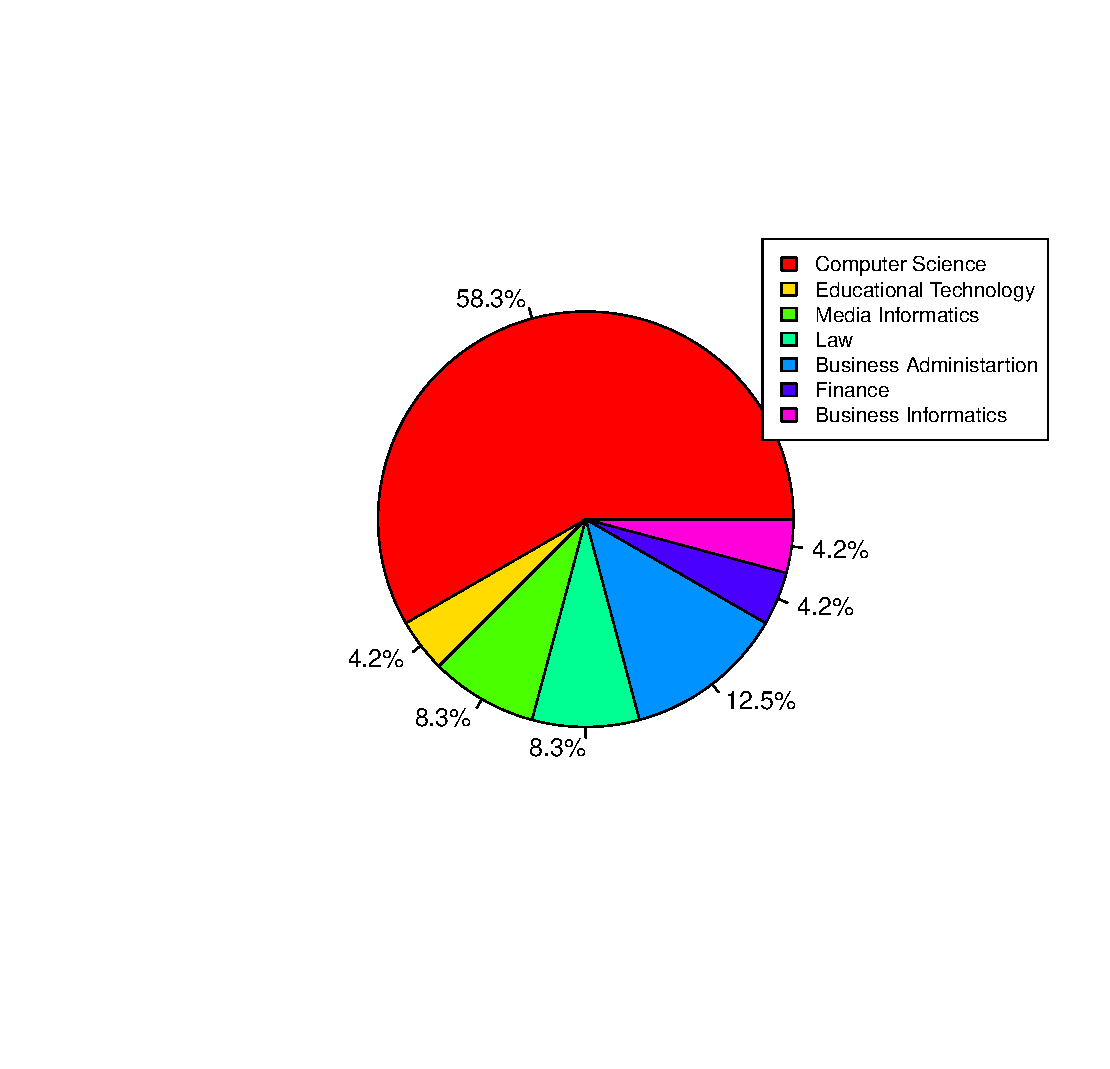
\includegraphics[scale=0.45]{RplotDemographicsFields.pdf}
      \caption{Participants' majors obtained from Demographics questionnaires}
      \label{fig:Dfields}
\end{figure}

\begin{figure}[H]
  \centering
    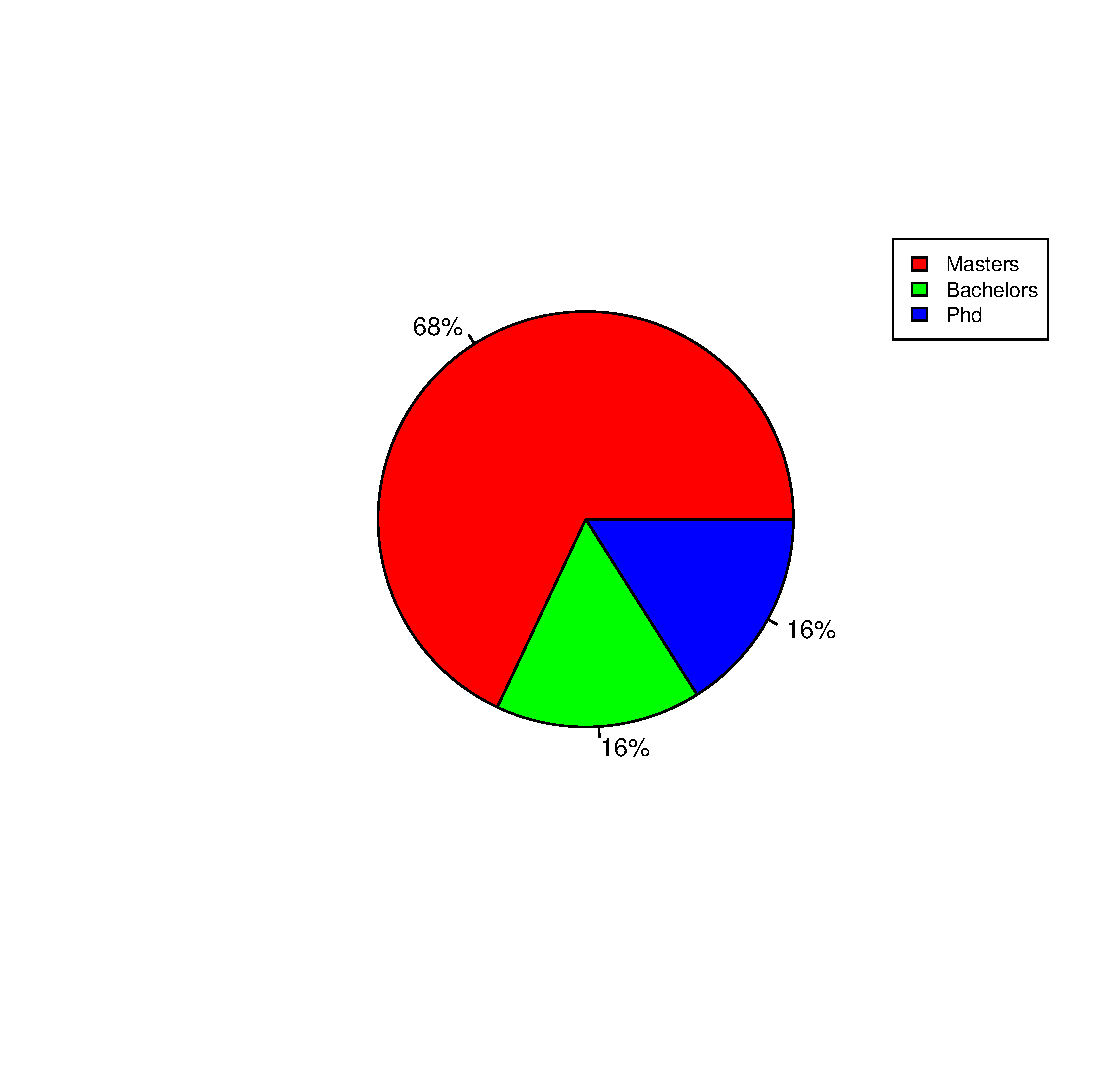
\includegraphics[scale=0.45]{RplotDemographicsStudyLevel.pdf}
      \caption{Participants' education level obtained from Demographics questionnaires}
      \label{fig:DstudyLevels}
\end{figure}

In the demographics form, participants also informed how frequently they used such devices as phones, smart lamps, tablets, and speakers (see Figure~\ref{fig:DdeviceUse} and Figure~\ref{fig:DdeviceUseInHours}). 

\begin{figure}[H]
  \centering
    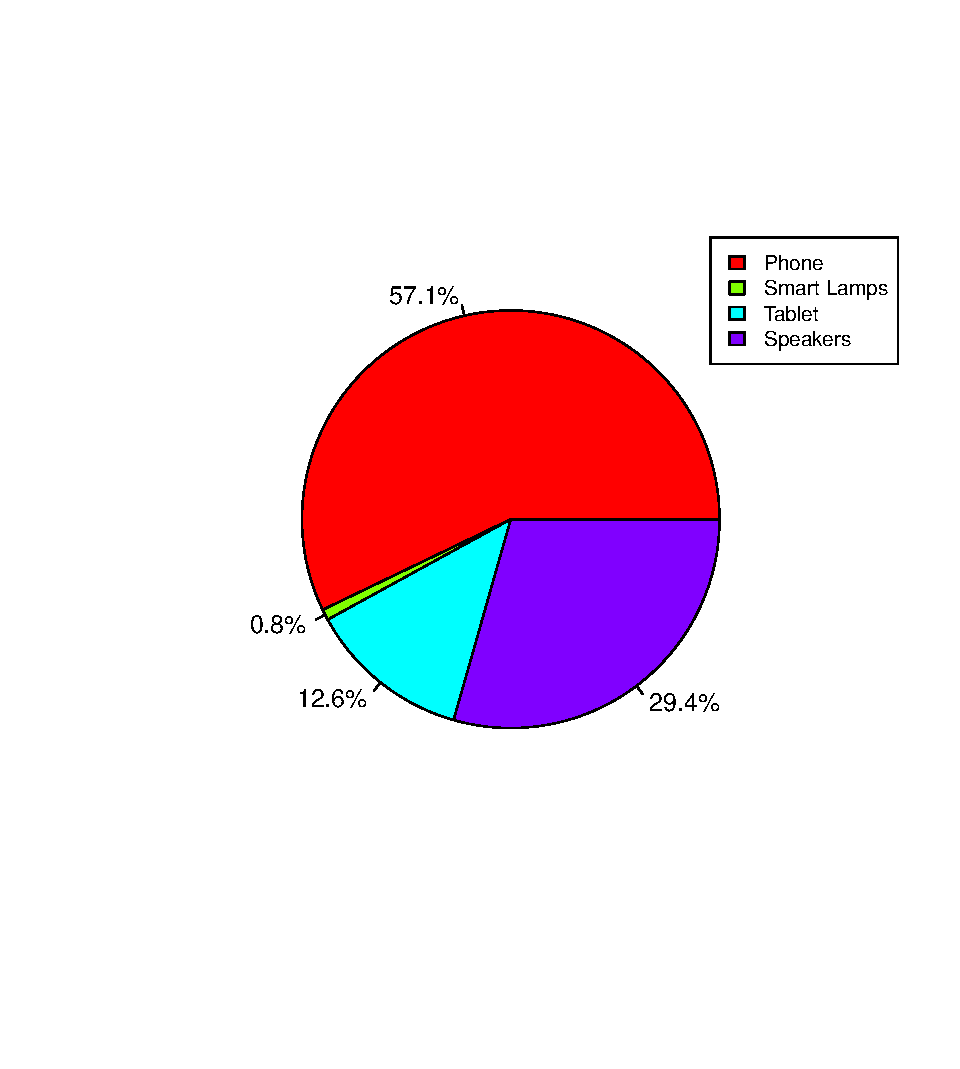
\includegraphics[scale=0.45]{RplotDemographicsDeviceUse.pdf}
      \caption{Participants' use of devices obtained from Demographics questionnaires}
      \label{fig:DdeviceUse}
\end{figure}

Overall, the experience level with above mentioned devices is listed in descending order: phone, speakers, tablet, and smart lamps. Figure~\ref{fig:DdeviceUseInHours} shows how many hours participants spend on these devices per day. The demographics questionnaire showed that the most popular device among our participants were phone with approximately 1/3 of participants who spent more than 6 hours on them. In all time ranges, the speakers were the second most used devices in comparison to the number of participants using of Tablet and Smart Lamps. 

\begin{figure}[H]
  \centering
    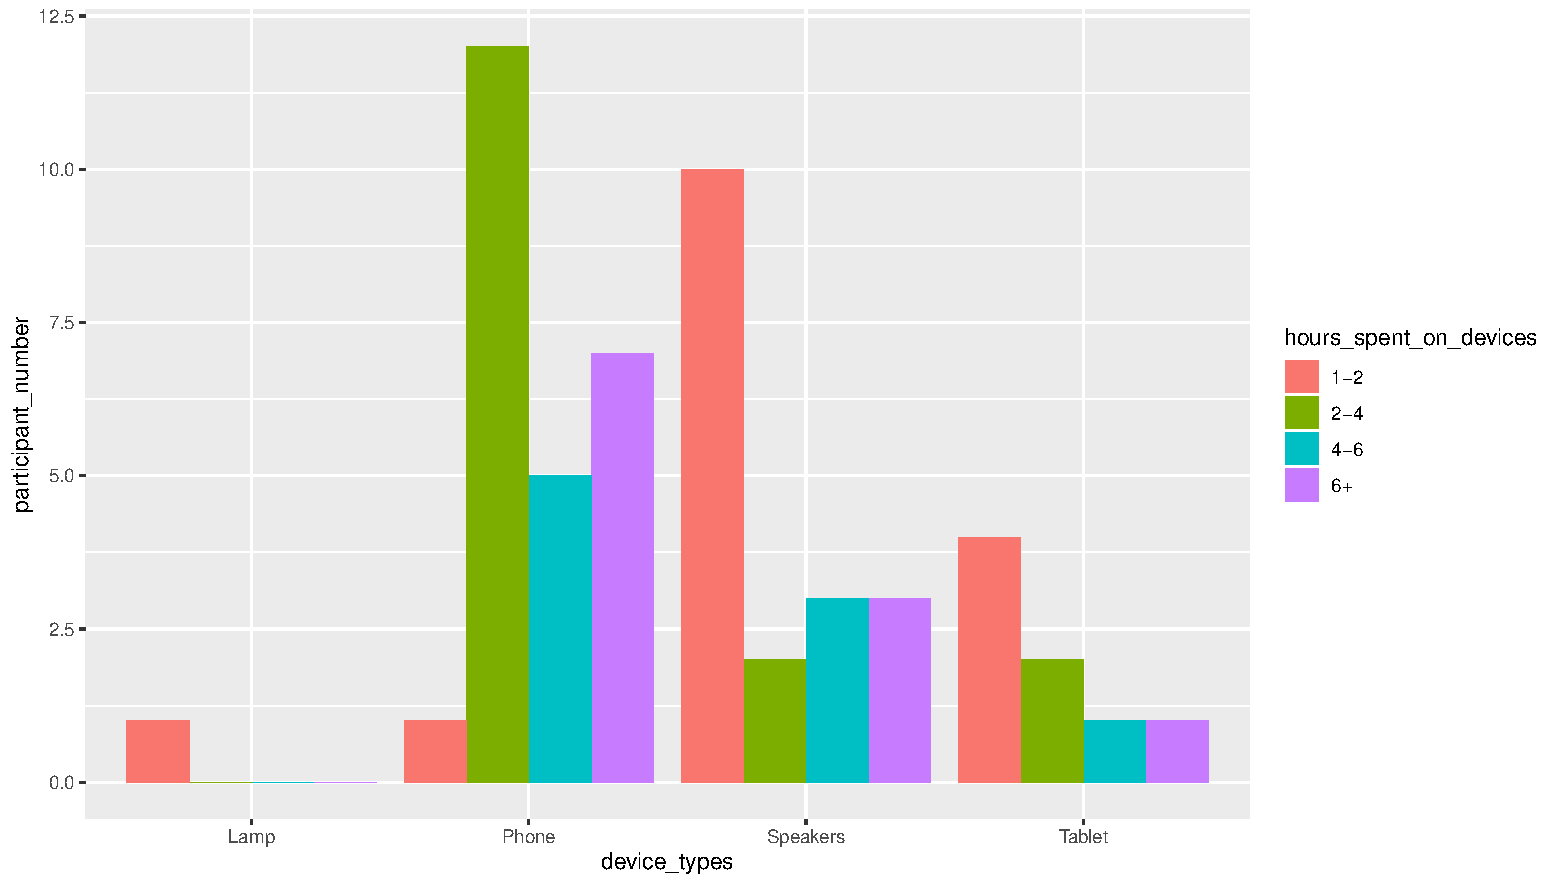
\includegraphics[scale=0.45]{RplotDemographicsDeviceUseInHours.pdf}
      \caption{Participants' device use in hours obtained from Demographics questionnaires}
      \label{fig:DdeviceUseInHours}
\end{figure}

In addition, Table~\ref{table:MusicFamiliarity} describes the participants’ preference of the music genres. The more fluent the participant would be with the music, the more rapid becomes the assessment of genre-specific features [Gjerdigen, R.O., Perrot, D., 2008. Scanning the dial: the rapid recognition of music genres]. Moreover, if the majority of participants prefer to listen or like certain genre of music, it may result in biased opinions. The mascot that triggers genre that they prefer may give participants more positive impression about their personality. Thus, the main reason of gathering data regarding participants' the music preferences was to see whether the liking factor affects the study or not. 
\par According to the One-Sample t-test with p>0.05, there was no significant effect of the participants’ music preference on the music genres that we chose for our study. Thus, we have insufficient evidence to conclude that one music genre is more preferable than the other. Meaning that, among the genres of music that we have chosen for our experiments, there were no distinguishably favorite genres and the participants had different music tastes (see Table~\ref{table:MusicFamiliarity}).

\begin{table}
\centering
\begin{tabular}{ | m{4.5em} | m{3em} | m{1em} | m{2em} | m{4em} | m{5.5em} | m{5em} |  } 
\hline
\multirow{2}{*}{} &
  \multicolumn{1}{| c}{ t-value} &\multicolumn{1}{| c}{df}  & \multicolumn{1}{| c}{mean} & \multicolumn{1}{| c}{p-value} & \multicolumn{2}{| c |}{95 percent confidence interval} \\
\hline
& 	&	&	  &  & lower & upper \\
\hline 
Country &	1 & 24 &	0.04 &	0.3273 &	- 0.04255594 & 0.12255594 \\
\hline 
Pop & 3.6742 &	 24 &	0.36	& 0.001195 &	0.1577801	& 0.5622199 \\
\hline 
Hip-hop	& 1.8091	& 24	& 0.12	& 0.08299	& - 0.01690354	& 0.25690354 \\
\hline 
Rap	&1&	24 &	0.04	& 0.3273 &	- 0.04255594&	0.12255594\\
\hline 
Jazz & 2.4495 & 24 &	0.2 & 	0.02198 & 	0.03148339 &	0.36851661\\
\hline 
Classic &	3.0551 &	24 &	0.28 &	0.005443 &	0.09084057	& 0.46915943\\
\hline 
Rock\&Roll	 & 1	& 24	& 0.04	& 0.3273	& - 0.04255594	& 0.12255594\\
\hline 

\end{tabular}
\caption{T-test for participants' familiarity with music genres used in our study}
\label{table:MusicFamiliarity}
\end{table}


\section{Procedure and Tasks}
When the experiment started, first, the participants were given an introductory paper describing the following aspects:
\begin{itemize}
  \item The implemented prototype introducing the devices used in our study
  \item The key idea of a study
  \item The purpose of the experiment
  \item The goal of the participants during experiment
  \item The number of phases and the overall duration of the experiment
\end{itemize}

Regardless of the introductory paper, the participant was allowed to ask open questions. After agreeing and signing the consent form (see appendix A), the main part of the experiment took place. 
\par In general, we have 4 phases for each of interaction types: Mascot-Mascot, Mascot-Lamps, Mascot-Tablet, Mascot-Speakers. The order of all phases were counterbalanced by using Latin Square. Each phase consists of 5 videos with a duration of 20 seconds, with the exception of Mascot-Speakers interactions where we have 9 videos with duration 40 seconds long. Moreover, for each participant, there were a different order of displaying the videos which are also randomized inside each phase based on the Latin Square. All phases and all videos within those phases were counterbalanced across all participants. Moreover, each participant was tested alone to ensure that the opinions of other participants do not affect their own. 
\par Before each phase, we describe the participant what kind of interaction they should expect from video and remind them their goals during that experiment. The goal is that, after watching short videos, participants will need to evaluate the personality of a Mascot according to the interaction that they have seen in the videos. When accomplishing watching the video, the participants were given a questionnaire (see appendix B) with 30 Likert scale questions and were asked to rank the personality trait on a scale of 'Strongly Inaccurate' to 'Strongly Accurate'. When this is done the experiment continues to the next video. After accomplishing watching all the videos in one phase, we move forward to the next phase. 
\par In addition, the only phase where the participants are given an extra phone is the Mascot-Mascot interaction phase, where two Mascots start to vibrate with a different duration based on the personality of approaching Mascot. Since it is difficult to see or hear the vibration from these videos, the phone runs an application to simulate the different levels of a vibration that we showed participants in the video. After watching the video, the participants were again given a questionnaire in order to assess the personality of a Mascot based on the video that they have seen and the vibration that they have felt.

\par After finishing the experiment, the participants were given a demographic questionnaire with general information about themselves and their preferences. The reason for giving this questionnaire at the end of the experiment was in order to not to affect the opinion of the participants. Giving personal questions up-front, respondents can feel concerned that their personal information is going to be linked to the experiment and therefore, knowing which characteristics will be taken into the account by the researchers, they may try to fit their responses to the demographic questions that they filled.
\par The experiment, overall, lasts from one hour to hour and a half, depending on the speed of participant to fill the questionnaires.

\section{Design of experiments}
\par It should be noted that as a design of the experiment we did not include a real-life interaction with devices, but instead, we showed participants videos containing the interaction between these devices. The main reason for that was the distraction of participants on various factors. 
\par From an implementation perspective, the application using BLE (low-energy Bluetooth) technology measures the distance between objects is highly accurate and precision, it can measure the distance from the phone to the beacon tag with a margin error of 1 cm which is a very good result. However, the position histories are saved every few seconds [Location Aware Tracking with Beacons Gary Mansell, Kevin Curran] and since the application measures the distance every millisecond, the current distance can only be saved after a few seconds. 
\par Moreover, the step of one person covers several centimeters at once, and the application calculates each of these centimeters at a time. Since asking participants to move slower or with small steps may distract them by focusing on their own behavior rather than on the assessment of the mascot's personality, we decided to use videos in our experiments. Moreover, having tested many other commercial applications that measures the distance between objects, we noticed the same limitation.
\par Another design decision was instead of showing one video with all interaction types, we split it into 5 short videos for Mascot-Lamp, Mascot-Table, Mascot-Mascot each and into 9 short videos for Mascot-Speakers cases. Even thought our prototype supports multi dimensional device interactions (i.e multiple mascots can interact with lamp, tablet, speakers and other mascots at the same time), we decided to split interaction types into four phases. The main goal was to help participant to focus on one interaction and make it easier for them to evaluate the personality of Mascot.

\section{Apparatus and Materials}
The experiment’s setup consisted of the following devices:
\begin{itemize}
  \item MacBook Pro running Mac OS Catalina (Version 10.15.2)
  \item 55-inch monitor with built-in speakers for music play
  \item Tablet to fill questionnaire in the google forms
  \item Nexus One for simulating the vibration during mascot-mascot interaction
\end{itemize}

As a survey tool for collecting data from participants, we used Google Form which consisted of the thirty Likert scale type questions scaling from 'Strongly Inaccurate' to 'Strongly Accurate' scales. Subsequently, in order to use obtained data in our statistical analysis, the questions from our survey tool were transformed in a more permanent form (i.e. four CSV files were generated, one for each phase).

\section{Design of a study}
The study consists of four case-studies: Mascot-Lamp, Mascot-Table, Mascot-Mascot and Mascot-Speakers interactions which, therefore, designed as four phases during experiments. The experiment was a within-subjects design where each participant tests all conditions within each phase. For example, for Mascot-Lamp phase each participant watch all five videos and evaluates the personality of a Mascot for each lighting color separately. The within-subjects in comparison to the between-subjects design can help us to reduce errors associated with individual differences. Individual participants have different backgrounds, contexts, levels of concentration and so on. The same participant interacting with all 4 phases, will affect the result in the same way which can the lower the probability that individual differences will skew the results. Moreover, the within-subject design requires fewer participants, which may lead us to the streamlined process of an experiment. 

\par In our study the independent variables (IVs) are factors that are triggered due to the behavior of a mascot. For each case-study, we have different number of IVs which are the followings:
\begin{itemize}
  \item For Mascot-Lamp case-study, there are five variable: turquoise, blood-red, yellow, orange and pink lighting colors
  \item For Mascot-Mascot case-study, there are five vibration levels varying from 100 to 500 milliseconds per time
  \item For Mascot-Speakers case-study, there are nine songs categorized to three variables: Sophisticated, Contemporary and Unpretentious categories
   \item For Mascot-Tablet case-study, there are five variable: yellow, orange, turquoise, blood-red and pink background screen colors
\end{itemize}

\par In fact, we do not compare case-studies with each other, namely, the interaction types has a more effect on the measurements of the personality trait of mascots. We consider one case as a separate study, where we only compare IVs.
\par Our dependent variable is the measurements of the personality traits based on the OCEAN model. The main research question that we asked: “Is the interpretation or the measure of the Mascot’s personality effected by these factors?”

\section{Measures}
As a measurements of the experiments we used questionnaires that were given after each video watch. Overall, there were 24 questionnaires with five questionnaires for each phase, except mascot-speakers interaction phase, where we had nine questionnaires. Each questionnaire consists of 30 questions portraying six facets of each personality based on NEO-PIP survey. The questionnaire items were answered using a Likert-scale (Very inaccurate, Inaccurate, neutral, Accurate, Very accurate). These questionnaires were given via Google Forms which are further transformed into cvs formats.




\chapter{Results}
\label{ch:results}
This chapter presents the statistical analysis of our study where the results
for each use case, namely, Mascot-Lamp, Mascot-Mascot, Mascot-Tablet, and
Mascot-Speakers interactions are reported in each section separately.
In each section, there are two subsections where we report statistical tests for two
studies: within personality trait and within condition such as lighting color, music
category, vibration level or screen color.
In our first study, we focus on each personality trait separately
and the difference between each state of conditions within that personality trait.
In the second study, we focus on each state of condition separately
and the difference between five personality traits within that condition state.

\begin{figure}[H]
    \centering
    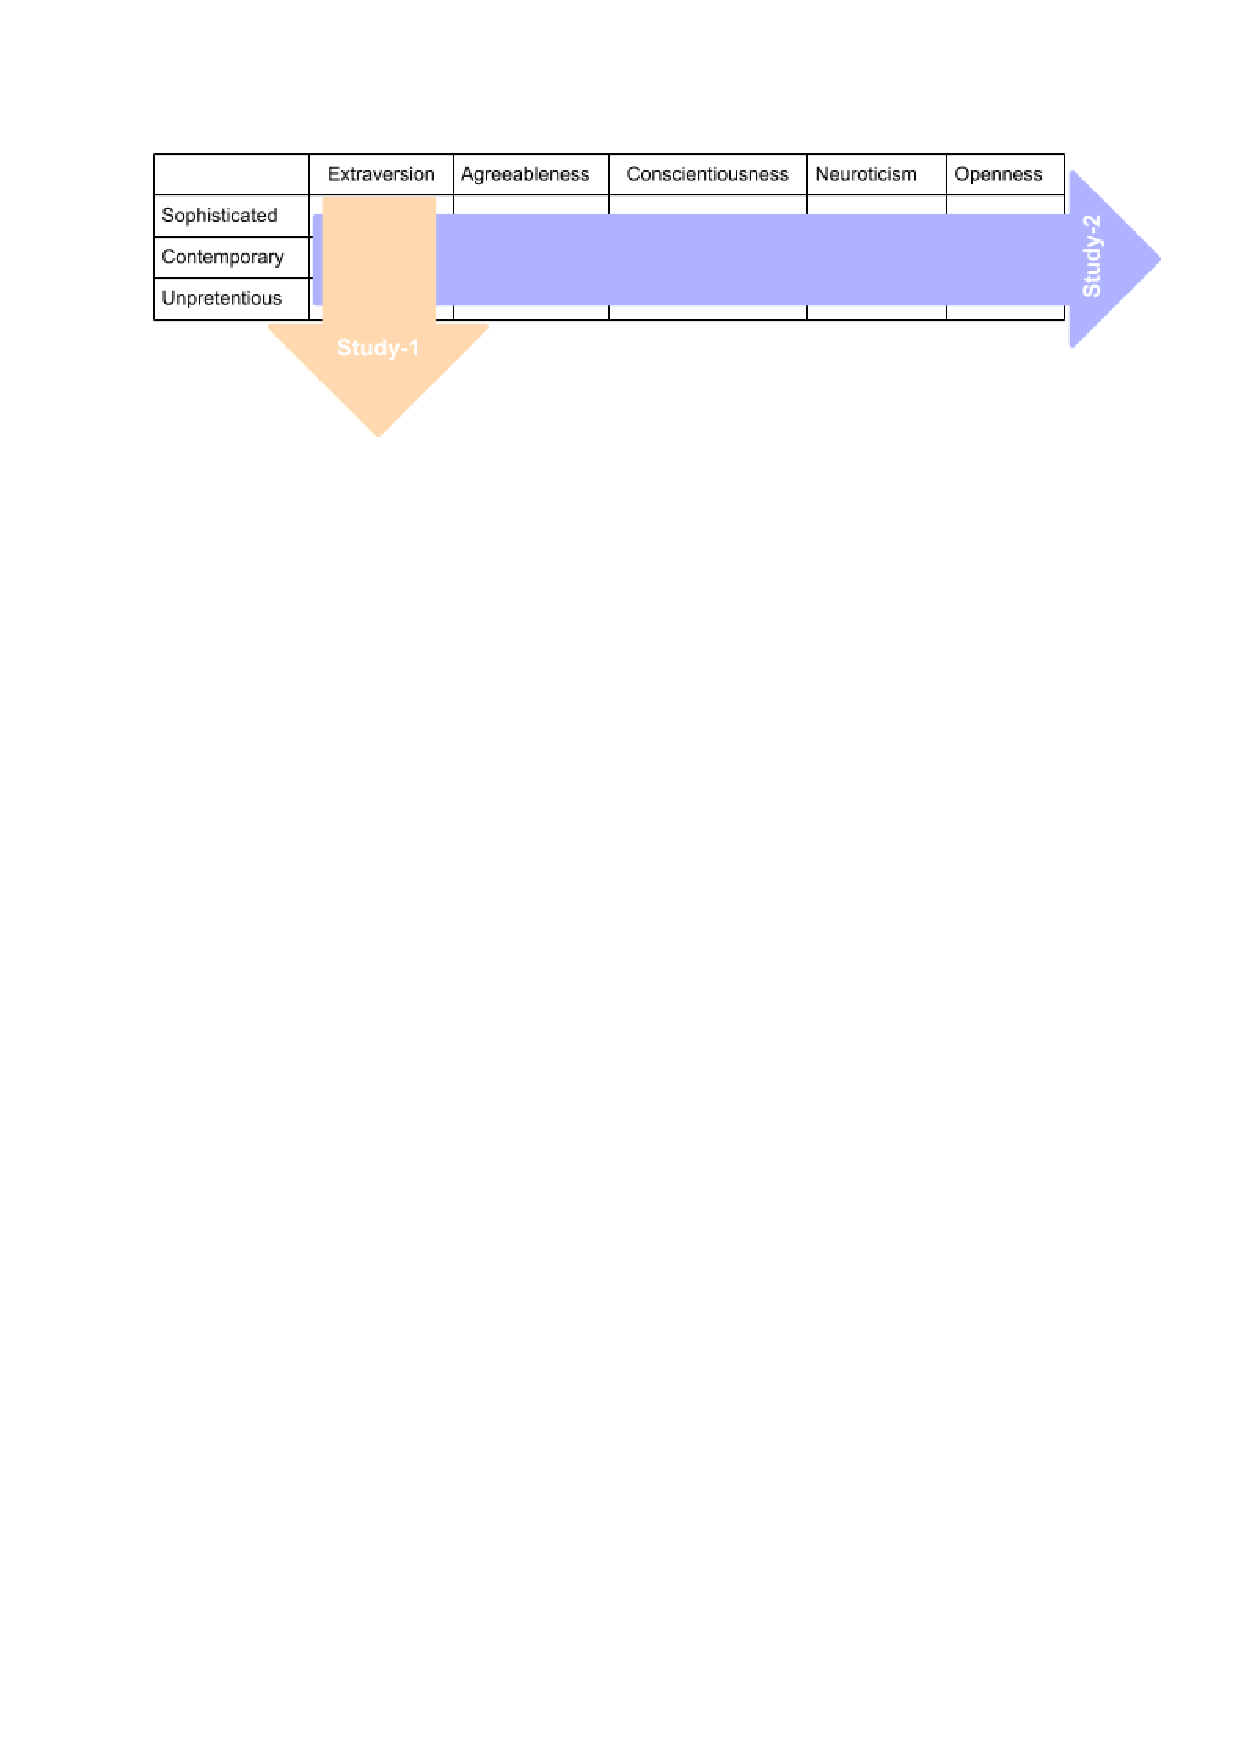
\includegraphics[scale=0.75]{StatSt12.pdf}
    \caption{Visual representation of compared groups in Study 1 and Study 2 for Mascot-Speakers interaction}
    \label{fig:Stat12}
\end{figure}
%%%%%%%%%%%%%%%%%%%%%%%%%%%%%%%%%%%%%%%%%%%%%%%%%%%%%%%%%%%%%%%%%%%%%%%%%%%%%%%%%%%%%%%%%%%%%%%%%%%%%%%%%%%%%%%%%%%%%%%%
\section{Analysis of Mascot-Lamp interaction}
\label{sec:m-l}
This section describes each personality trait that Mascot was assigned in terms of
the effect of the lighting color in evaluating them.
The factors that we compare for Mascot-Lamp interaction are orange, turquoise,
yellow, blood-red and pink lighting colors.
Since the data that we gathered are ordinal and we do not assume that the outcome
will be normally distributed, we focused on non-parametric tests for all case studies.
Moreover, since each case-study consists of more than two compared groups
(i.e in case of Mascot-Lamp interaction we compare five colors with each other)
and compare data against within-subject factor (i.e each participant tested all five conditions),
we decided to use Friedman test followed by the Wilcoxon Signed-rank test.
In both studies, we analyze the effect of the lighting color on how the mascot’s personality is measured.
The first study analyzes this effect within each personality trait, particularly, we consider each
personality trait and the effects of each color on participant's measurements of Mascot's personality.
The second study considers this effect within each color condition,
namely how each personality trait is assessed differently within one color condition.
For each study Wilcoxon test compare 10 groups with each other which makes 20 compared groups in total.
Since, in our study, we have a large number of statistical tests, some of the results may have p<0.05 purely by chance.
Thus, in order to control family wise error rate, we use Bonferroni correction which will
divide all p-values in 20 (the number of compared groups for both studies).
Finally, at the end of each subsections, we show a graphical display of the results from each study.
Subsection~\ref{subsec:MLstudy1} describes the results for within personality study and
subsection~\ref{subsec:MLstudy2} for within lighting color study.

%%%%%%%%%%%%%%%%%%%%%%%%%%%%%%%%%%%%%%%%%%%%%%%%%%%%%%%%%%%%%%%%%%%
\subsection{Analysis of within personality trait study}
\label{subsec:MLstudy1}
In the first study, we test the effect of all predefined lighting colors on the measurements of each personality trait.
Friedman tests reported in Table~\ref{table:friedmanML1} reveal a significant impact of lighting colors on the perception
of the personality trait of mascots with p < 0.01.

\par\textbf{Extraversion.}
According to Table~\ref{table:friedmanML1}, lighting colors significantly
influenced the measurements of Extraversion personality.
Figure~\ref{fig:ML1} reports where exactly this effect is concentrated.
Based on Wilcoxon tests, there are six groups of colors affecting the
measurements of Extraversion personality with p<0.01.
In addition, yellow showed significant difference in rating extraversion
comparing to turquoise, blood-red and pink lighting colors.
Participants rated Mascot's personality trait based on six facets of five
personality trait which makes in total 30 facets.
They rated the mascot that triggered yellow lighting color high on being
friendly, gregarious, assertive, energetic, excitement seeking and
cheerful in comparison to mascot that triggered blood-red, turquoise and pink colors.
All above mentioned facets represent extraversion personality trait (see Table--facets).
Thus, participants rated the mascot interacting with yellow lighting to convey extraversion personality.
In contrast, the mascot interaction with blood-red lighting was
rated very low on being extravert (see Figure~\ref{fig:ML1}).
This is also reported in Table~\ref{table:medianML1}, the blood-red color having
the lowest median (Med = 1.7, Max = , Min = ) and yellow having the highest
value (Med = 3.7, Max = , Min = ).

\par\textbf{Agreeableness.}
There is a significant impact of lighting colors and the participants'
measurements of agreeableness personality with p<0.01 (see Table~\ref{table:friedmanML1})
According to Figure~\ref{fig:ML1}, mascot triggered blood-red and orange lighting
were rated very low on being agreeable (padj<0.01).
Moreover, Table~\ref{table:medianML1} shows that in comparison to all other colors,
blood-red color has the smallest median values with Med = 2.0, Min = , Max = .
The median values, in descending order, for pink, turquoise and yellow lights are
approximately similar (Med = 4.0, Med = 3.5 and Med = 3.7).

\par\textbf{Conscientiousness.}
Friedman test shows statistically significant effect of all predefined lighting colors
on the ratings of Conscientiousness personality (see Table~\ref{table:friedmanML1}).
Wilcoxon tests show that effect is noticeable when we compare mascot that trigger
blood-red and orange with ones that triggered turquoise, yellow, pink colors (see Figure~\ref{fig:ML1}).
In fact, the mascot interacting with blood-red and orange lighting were assessed
as being very low on conscientious personality trait.
Table~\ref{table:medianML1} indicates that blood-red has a lowest median (Med = 2.2), whereas turquoise, pink and
yellow have relatively similar high medians (Med = 3.7, Med = 3.5, Med = 3.5 respectively in descending order).
The latest values shows that the mascot triggering these colors were assessed high on having
orderly, dutiful, disciplined and other facets that constitute conscientiousness personality.

\par\textbf{Neuroticism.}
Overall, there is an impact of predefined colors on the rating's of Neuroticism
personality with p<0.01 reported in Table~\ref{table:friedmanML1}.
Blood-red showed a significant difference in rating Neuroticism comparing
to all other colors with padj<0.01 after Bonferroni correction (see Figure~\ref{fig:ML1}).
Moreover, blood-red presented the highest median value (Med = , Max = , Min = ) (see Table~\ref{table:medianML1}).

\par\textbf{Openness.}
There is a significant difference of all colors within openness personality
with p<0.01 (see Table~\ref{table:friedmanML1}).
Moreover, the main differences are concentrated between yellow and pink, yellow and blood-red,
blood-red and orange with padj<0.01 (see Figure~\ref{fig:ML1}).
Table~\ref{table:medianML1} shows the similarity of the median values for all colors concentrating around neutral attitude for mascot
being measured as openness which is represented by median close to 3.

Figure indicates only significant comparisons with p<0.05.
We report p-values adjusted after Bonferroni correction for more
detailed information see Table--wilcoxon in Appendix.

\begin{longtable}{ |p{3cm}| p{1cm}|p{0.5cm}|p{1.7cm}| }
    \captionsetup{width=13.5cm}
    \caption{The results from Friedman test for all Five Personality traits in case of Mascot-Lamp interaction }
    \label{table:friedmanML1} \\
    \hline
    \multicolumn{1}{| c}{\textbf{Personality trait }}
    & \multicolumn{1}{| c}{\textbf{$\chi^2$}}
    & \multicolumn{1}{| c}{\textbf{df}}
    & \multicolumn{1}{| c |}{\textbf{p}}  \\
    \hline
    \endfirsthead
    \multicolumn{4}{c}%
    {\tablename\ \thetable\ -- \textit{Continued from previous page}} \\
    \hline
    \multicolumn{1}{| c}{\textbf{Personality trait }}
    & \multicolumn{1}{| c}{\textbf{$\chi^2$}}
    & \multicolumn{1}{| c}{\textbf{df}}
    & \multicolumn{1}{| c |}{\textbf{p}}  \\
    \hline
    \endhead
    \hline \multicolumn{4}{r}{\textit{Continued on next page}} \\
    \endfoot
    \hline
    \endlastfoot
    Extraversion		&39.959	&4	& p<0.01 \\
    Agreeableness		&56.448	&4	& p<0.01 \\
    Conscientiousness	&25.847	&4	& p<0.01\\
    Neuroticism		&52.377 	&4	& p<0.01 \\
    Openness			&18.156	&4	& p<0.01 \\
    \hline
\end{longtable}

\begin{table}[H]
    \renewcommand{\arraystretch}{1.2}
    \caption{Some Caption Y is yellow, O is orange \ldots}
    \label{table:medianML1}
    \begin{center}
        \begin{tabular}{p{0.05\textwidth}|
        p{0.025\textwidth}|p{0.025\textwidth}|p{0.025\textwidth}|p{0.025\textwidth}|p{0.025\textwidth}||
        p{0.025\textwidth}|p{0.025\textwidth}|p{0.025\textwidth}|p{0.025\textwidth}|p{0.025\textwidth}||
        p{0.025\textwidth}|p{0.025\textwidth}|p{0.025\textwidth}|p{0.025\textwidth}|p{0.025\textwidth}|}
            \cline{2-16}
            & \multicolumn{5}{c||}{\textbf{Extraversion}} & \multicolumn{5}{c||}{\textbf{Agreeableness}}
            & \multicolumn{5}{c|}{\textbf{Conscientiousness}} \\
            \cline{2-16}
                            & Y & O & T & B & P 			    & Y & O & T & B & P  	 	& Y & O & T & B & P     \\
            \cline{2-16}
            \textbf{Min}  	& 2.3 & 2.3 & 1.8 & 1.0 & 1.7 		& 1.8 & 1.0 & 2.0 & 1.0 & 2.5  	& 1.3 & 1.8 & 1.7 & 1.2 & 2.0  \\
            \textbf{Med} 	& 3.7 & 3.0 & 2.7 & 1.7 & 2.8 		& 3.7 & 2.3 & 3.5 & 2.0 & 4.0  	& 3.5 & 2.5 & 3.7 & 2.2 & 3.5  \\
            \textbf{Max}	& 4.8 & 4.8 & 4.2 & 4.5 & 3.7 		& 5.0 & 3.3 & 5.0 & 3.8 & 5.0  	& 4.8 & 3.3 & 5.0 & 4.7 & 5.0 \\
            \cline{2-16}
            \cline{2-11}
            &  \multicolumn{5}{|c||}{\textbf{Neuroticism}} & \multicolumn{5}{|c||}{\textbf{Openness}} \\
            \cline{2-11}
                            & Y & O & T & B & P 			& Y & O & T & B & P    		\\
            \cline{2-11}
            \textbf{Min} 	& 1.0 & 1.0 & 1.0 & 3.2 & 1.0 		& 1.5 & 1.7 & 2.3 & 1.2 & 1.5 	\\
            \textbf{Med}    & 2.1 & 2.5 & 2.0 & 4.3 & 1.7 	    & 3.5 & 3.0 & 2.8 & 2.7 & 2.8 	\\
            \textbf{Max}  	& 3.3 & 3.5 & 3.5 & 5.0 & 3.3 		& 5.0 & 4.7 & 3.7 & 4.0 & 4.0  	\\
            \cline{2-11}
        \end{tabular}
    \end{center}
\end{table}

\begin{figure}[H]
    \centering
    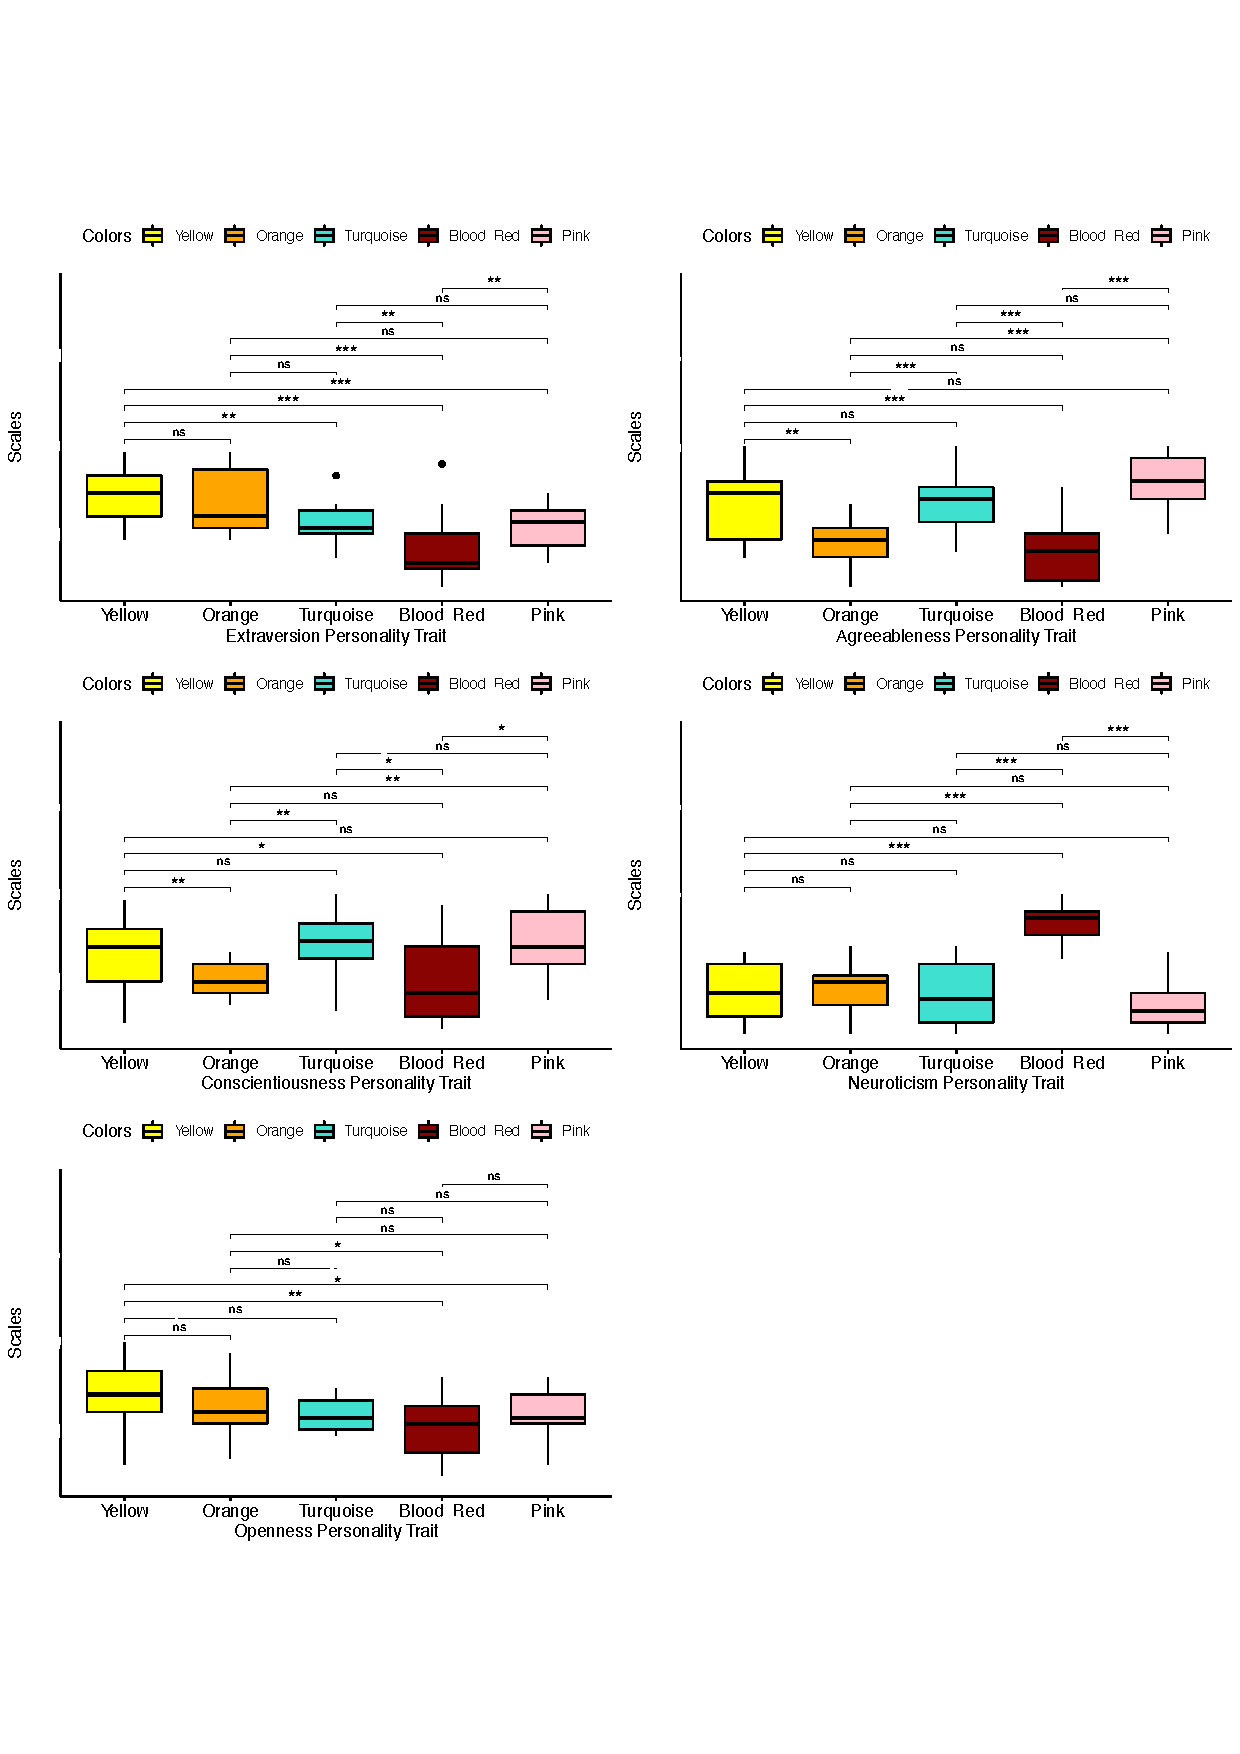
\includegraphics[scale=0.55]{Study1(M-L).pdf}
    \caption{A boxplot for Mascot-Lamp interaction in Study-1}
    \label{fig:ML1}
\end{figure}

%%%%%%%%%%%%%%%%%%%%%%%%%%%%%%%%%%%%%%%%%%%%%%%%%%%%%%%%%%%%%%%%%%%
\subsection{Analysis of within lighting color study}
\label{subsec:MLstudy2}
The second study considers effect of lighting color on how each
personality trait is assessed within one color condition.

\par\textbf{Yellow.}
Friedman test showed a significant difference of the ratings each personality trait
within yellow lighting color with p<0.01, df=4 (see Table~\ref{table:friedmanML2}).
The difference is concentrated on Neuroticism personality which is rated very low when mascot triggers yellow light.
According to Figure~\ref{fig:ML2}, 80\% of scores given for extraversion, agreeableness,
conscientiousness, and openness were higher than all scores given for neurotic personality.
In addition, the similarity of the median values for all personality traits except
neuroticism (Med = 3.7, Med = 3.7, Med = 3.5, Med = 3.5) reveals a small effect of yellow
color on these four personality traits (see Table~\ref{table:medianML2}).

\par\textbf{Orange.}
There is a statistically substantial difference between personality trait measurements within
orange color with p<0.01, df=4 (see Table~\ref{table:friedmanML2}).
When orange color is triggered, the mascot with Extraversion and Openness traits
show distinguishable ratings in comparison to all other personalities with p<0.05 (see Figure~\ref{fig:ML2}).
Moreover, tests did not show any significant differences between extraversion (Med = 3.0, Max = , Min = )
and openness (Med = 3.0, Max = , Min = ) within orange color (see Figure~\ref{fig:ML2} and Table~\ref{table:medianML2}).
However, the median values of extraversion and openness are higher compared to values of all other personality traits.

\par\textbf{Turquoise.}
Overall all personality traits shows different results when light was transformed to turquoise color
with p<0.01, df=4 (see Table~\ref{table:friedmanML2}).
Wilcoxon test reveals that when the turquoise is displayed, the agreeableness and conscientiousness
personality traits are substantially distinguishable from other personality traits with p<0.05 (see Figure~\ref{fig:ML2}).
Both, conscientiousness and agreeableness personalities measured high when Mascot triggers  turquoise color.
However, these two personalities are not distinguishable within turquoise color.
In Spite of that fact, the median value of conscientiousness (Med = 3.7)is slightly higher than
agreeableness (Med = 3.5) (see Table~\ref{table:medianML2}), high p-values indicate that the measurements of
these two personality traits are not differ when turquoise color is triggered.

\par\textbf{Blood-red.}
lighting color reveals significant difference in measurements of all personality traits
with p<0.01, df=4 (see Table~\ref{table:friedmanML2}).
Moreover, according to Figure~\ref{fig:ML2}, there is an excellent separation of neuroticism boxplot from all other personality traits.
Table~\ref{table:medianML2} shows very high median value for Neuroticism compared to other
personality traits with Med = , Min =  and Max = .

\par\textbf{Pink.}
There is a significant difference in rating Mascots' personality when the pink light is
triggered with p<0.01, df=4 (see Table~\ref{table:friedmanML2}).
According to the Figure~\ref{fig:ML2}, pink lighting color shows a significant effect on agreeableness
and conscientiousness with p<0.01 comparing to extraversion, neuroticism and openness personality traits.
Based on the medians reported in Table~\ref{table:medianML2}, agreeableness has the
highest (Med = 4.0) in contrast to the neuroticism which has a lowest value (Med = 1.7).

\begin{longtable}{ |p{1.7cm}| p{1cm}|p{0.5cm}|p{1.7cm}| }
    \captionsetup{width=13.5cm}
    \caption{The results from Friedman test for all Five Personality traits in case of Mascot-Lamp interaction}
    \label{table:friedmanML2} \\
    \hline
    \multicolumn{1}{| c}{\textbf{Personality trait }}
    & \multicolumn{1}{| c}{\textbf{$\chi^2$}}
    & \multicolumn{1}{| c}{\textbf{df}}
    & \multicolumn{1}{| c |}{\textbf{p}}  \\
    \hline
    \endfirsthead
    \multicolumn{4}{c}%
    {\tablename\ \thetable\ -- \textit{Continued from previous page}} \\
    \hline
    \multicolumn{1}{| c}{\textbf{Personality trait }}
    & \multicolumn{1}{| c}{\textbf{$\chi^2$}}
    & \multicolumn{1}{| c}{\textbf{df}}
    & \multicolumn{1}{| c |}{\textbf{p}}  \\
    \hline
    \endhead
    \hline \multicolumn{4}{r}{\textit{Continued on next page}} \\
    \endfoot
    \hline
    \endlastfoot
    Yellow		&23.566	&4	&p<0.01 \\
    Orange		&38.178	&4	&p<0.01\\
    Turquoise		&37.123	&4	&p<0.01 \\
    Blood-red		&45.475	&4	&p<0.01 \\
    Pink			&60.082	&4	&p<0.01 \\
    \hline
\end{longtable}

\begin{table}[H]
    \renewcommand{\arraystretch}{1.2}
    \caption{Some Caption Y is yellow, O is orange \ldots}
    \label{table:medianML2}
    \begin{center}
        \begin{tabular}{p{0.05\textwidth}|
        p{0.025\textwidth}|p{0.025\textwidth}|p{0.025\textwidth}|p{0.025\textwidth}|p{0.025\textwidth}||
        p{0.025\textwidth}|p{0.025\textwidth}|p{0.025\textwidth}|p{0.025\textwidth}|p{0.025\textwidth}||
        p{0.025\textwidth}|p{0.025\textwidth}|p{0.025\textwidth}|p{0.025\textwidth}|p{0.025\textwidth}|}
            \cline{2-16}
            & \multicolumn{5}{c||}{\textbf{Yellow}} & \multicolumn{5}{c||}{\textbf{Orange}}
            & \multicolumn{5}{c|}{\textbf{Turquoise}} \\
            \cline{2-16}
                            & E & A & C & N & O 			    & E & A & C & N & O   	 	& E & A & C & N & O      \\
            \cline{2-16}
            \textbf{Min}  	& 2.3 & 1.8 & 1.3 & 1.0 & 1.5 		& 2.3 & 1.0 & 1.8 & 1.0 & 1.7  	& 1.8 & 2.0 & 1.7 & 1.0 & 2.3  \\
            \textbf{Med} 	& 3.7 & 3.7 & 3.5 & 2.2 & 3.5 		& 3.0 & 2.3 & 2.5 & 2.5 & 3.0  	& 2.7 & 3.5 & 3.7 & 2.0 & 2.8  \\
            \textbf{Max}	& 4.8 & 5.0 & 4.8 & 3.3 & 5.0 		& 4.8 & 3.3 & 3.3 & 3.5 & 4.7  	& 4.2 & 5.0 & 5.0 & 3.5 & 3.7 \\
            \cline{2-16}
            \cline{2-11}
            &  \multicolumn{5}{|c||}{\textbf{Blood-red}} & \multicolumn{5}{|c||}{\textbf{Pink}} \\
            \cline{2-11}
            & E & A & C & N & O 			& E & A & C & N & O     		\\
            \cline{2-11}
            \textbf{Min} 	& 1.0 & 1.0 & 1.2 & 3.2 & 1.2 		& 1.7 & 2.5 & 2.0 & 1.0 & 1.5 	\\
            \textbf{Med}    & 1.7 & 2.0 & 2.2 & 4.3 & 2.7 	    & 2.8 & 4.0 & 3.5 & 1.7 & 2.8 	\\
            \textbf{Max}  	& 4.5 & 3.8 & 4.7 & 5.0 & 4.0 		& 3.7 & 5.0 & 5.0 & 3.3 & 4.0  	\\
            \cline{2-11}
        \end{tabular}
    \end{center}
\end{table}

\begin{figure}[H]
    \centering
    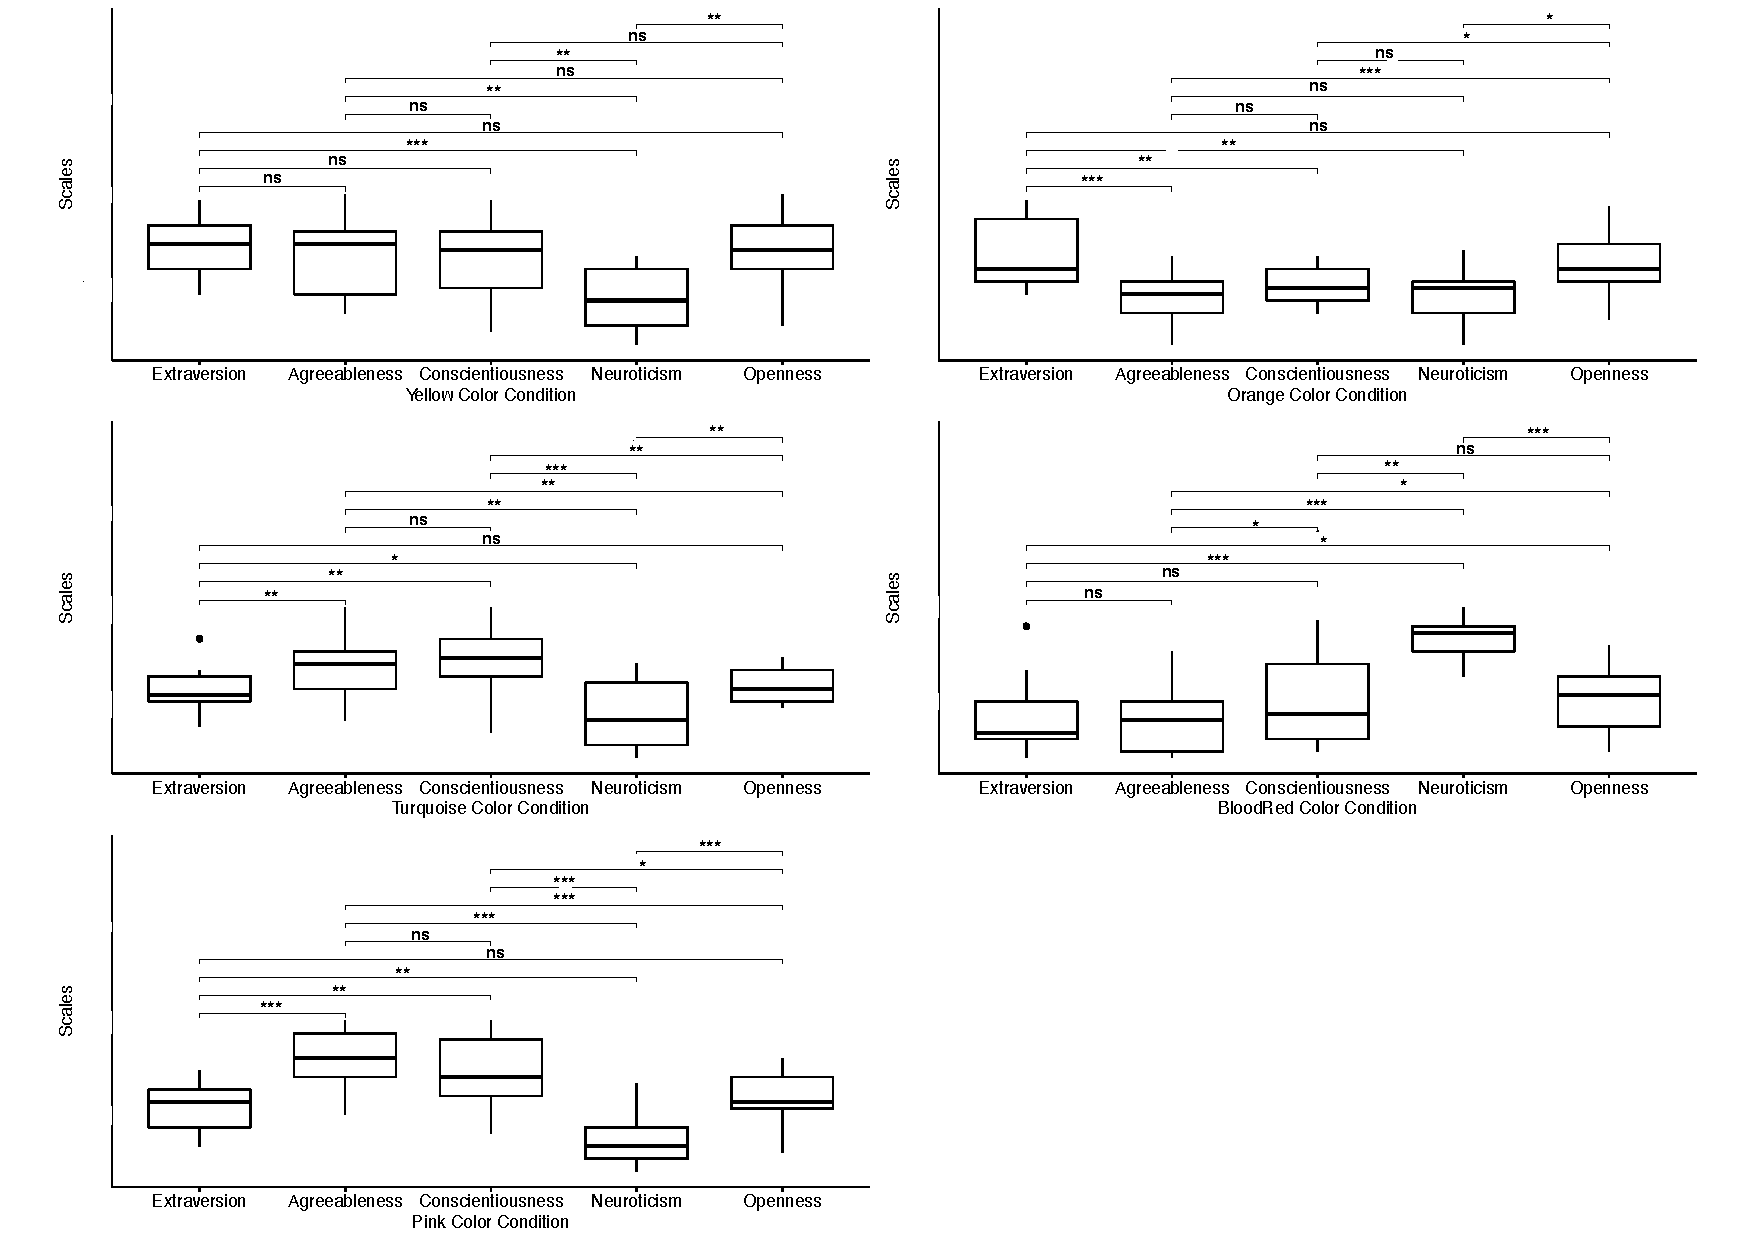
\includegraphics[scale=0.45]{Study2(M-L).pdf}
    \caption{A boxplot for Mascot-Lamp interaction in Study-1}
    \label{fig:ML2}
\end{figure}

%%%%%%%%%%%%%%%%%%%%%%%%%%%%%%%%%%%%%%%%%%%%%%%%%%%%%%%%%%%%%%%%%%%%%%%%%%%%%%%%%%%%%%%%%%%%%%%%%%%%%%%%%%%%%%%%%%%%%%%%
\section{Analysis of Mascot-Speakers interaction}
\label{sec:m-s}
This section includes the Mascot-Speakers case-study, where we analyze the effect music genre
has on the assessment of the Mascots' personality traits.
As we discussed in Chapter~\ref{ch:concept}, our choice of the music genre is based on the MUSIC pattern.
For statistical analysis, we examine the effect of
each category by distributing genres into three categories as the following:
\begin{itemize}
  \item Sophisticated:  jazz, classical and contemporary adult
  \item Contemporary: rap, soul, and rap
  \item Unpretentious: pop, rock\&roll / country and bluegrass
\end{itemize}

The factor that we compare  fo Mascot-Speakers interaction are sophisticated, contemporary and unpretentious music.
In subsection~\ref{subsec:MSstudy1} we analyse within personality trait study,
where we compare the effect of all three music categories on each personality trait.
In subsection~\ref{subsec:MSstudy2}, we compare the same effect within music category.
In case if one music category conveys multiple personality traits, the second study will compare
these traits within that music category and will result in personality with the highest rate.

%%%%%%%%%%%%%%%%%%%%%%%%%%%%%%%%%%%%%%%%%%%%%%%%%%%%%%%%%%%%%%%%%%%
\subsection{Analysis of within personality trait study}
\label{subsec:MSstudy1}
In this subsection, we report a statistical analysis of how the impact of the music category varies within each
personality trait.

\par\textbf{Extraversion.} Table~\ref{table:friedmanMS1}
Friedman tests shows significant effect of all predefined music categories on the
ratings of Extraversion personality with p<0.01, df=2 (see Table~\ref{table:medianMS1}).
Wilcoxon tests revealed that significant difference is concentrated on Contemporary music
with all other categories with padj<0.01 (see Figure~\ref{fig:MS1}).
According to Table~\ref{table:medianMS1}, Contemporary category has the highest median with Med = .

\par\textbf{Agreeableness.}
All these categories significantly influenced participants' measurements of Mascot's
agreeableness personality trait with p<0.01, df=2 (see Table~\ref{table:medianMS1}).
The main difference fault in Sophisticated and Contemporary, and Contemporary
and Unpretentious groups with p<0.01.
According to Figure~\ref{fig:MS1}, it discriminates most of the Contemporary samples from
samples of the other two categories having very low ratings on conveying Agreeableness personality trait.

\par\textbf{Conscientiousness.}
There is a significantly difference of all music categories within conscientiousness
personality trait with p<0.05, df=2 (see Table~\ref{table:medianMS1}.
Similar to Agreeableness personality, when Contemporary music was played, ratings
for Mascot attributing Conscientiousness personality traits were significantly low
in comparison to all other music types with p<0.05, df=2 (see Figure~\ref{fig:MS1}).
Scores for Mascot having Conscientiousness personality traits increased sharply during listening Sophisticated
(median = 3.2) and Unpretentious (median = 3.2) music in comparison to scores for Contemporary music (median = 2.8)
The Wilcoxon test confirms the statistically significant difference between Sophisticated and Contemporary
(padj<0.01), and Unpretentious and Contemporary (padj<0.05) categories.

\par\textbf{Neuroticism.}
Overall all three categories has an effect on the measurement of Mascot's neuroticism
personality with p<0.01, df=2 (see Table~\ref{table:medianMS1}).
Table~\ref{table:medianMS1} shows that the scores given for Contemporary music while assessing
Neuroticism personality traits are highest with Med = 3.1 compared to other two categories.
Moreover, there are two significant differences between Sophisticated and Contemporary,
and Contemporary and Unpretentious music with padj<0.01 (see Figure~\ref{fig:MS1}).

\par\textbf{Openness.}
Table~\ref{table:medianMS1} reveals a substantial difference between all three music types
within openness personality trait.
Particularly, there is a good separation of Sophisticated with median = 3.8 and max = 4.9
from other music categories (see Table~\ref{table:medianMS1}).
The samples for the mascot with a current personality trait are well behaved.
There is a large difference between Sophisticated and Contemporary, and Sophisticated
and Unpretentious which is also confirmed with the Bonferroni correction with p<0.01 (see Figure~\ref{fig:MS1}).

\begin{longtable}{ |p{3cm}| p{1cm}|p{0.5cm}|p{1.7cm}| }
    \captionsetup{width=13.5cm}
    \caption{The results from Friedman test for all Five Personality traits in case of Mascot-Speakers interaction}
    \label{table:friedmanMS1} \\
    \hline
    \multicolumn{1}{| c}{\textbf{Personality trait }}
    & \multicolumn{1}{| c}{\textbf{$\chi^2$}}
    & \multicolumn{1}{| c}{\textbf{df}}
    & \multicolumn{1}{| c |}{\textbf{p}}  \\
    \hline
    \endfirsthead
    \multicolumn{4}{c}%
    {\tablename\ \thetable\ -- \textit{Continued from previous page}} \\
    \hline
    \multicolumn{1}{| c}{\textbf{Personality trait }}
    & \multicolumn{1}{| c}{\textbf{$\chi^2$}}
    & \multicolumn{1}{| c}{\textbf{df}}
    & \multicolumn{1}{| c |}{\textbf{p}}  \\
    \hline
    \endhead
    \hline \multicolumn{4}{r}{\textit{Continued on next page}} \\
    \endfoot
    \hline
    \endlastfoot
    Extraversion		&21.44	&2	&p<0.01 \\
    Agreeableness		&29.01	&2	&p<0.01\\
    Conscientiousness	&6.4536	&2	&p<0.05\\
    Neuroticism		&15.122 	&2	&p<0.01 \\
    Openness			&25.838	&2	&p<0.01 \\
    \hline
\end{longtable}

\begin{table}[H]
    \renewcommand{\arraystretch}{1.2}
    \caption{Some Caption Y is yellow, O is orange \ldots}
    \label{table:medianMS1}
    \begin{center}
        \begin{tabular}{p{0.05\textwidth}|
        p{0.025\textwidth}|p{0.025\textwidth}|p{0.025\textwidth}||
        p{0.025\textwidth}|p{0.025\textwidth}|p{0.025\textwidth}||
        p{0.025\textwidth}|p{0.025\textwidth}|p{0.025\textwidth}||
        p{0.025\textwidth}|p{0.025\textwidth}|p{0.025\textwidth}||
        p{0.025\textwidth}|p{0.025\textwidth}|p{0.025\textwidth}|}
            \cline{2-16}
            & \multicolumn{3}{c||}{\textbf{E}} & \multicolumn{3}{c||}{\textbf{A}}
            & \multicolumn{3}{c||}{\textbf{C}} &  \multicolumn{3}{c||}{\textbf{N}} & \multicolumn{3}{c|}{\textbf{O}} \\
            \cline{2-16}
                            & S & C & U  			& S & C & U   	 	& S & C & U      & S & C & U  		& S & C & U     		\\
            \cline{2-16}
            \textbf{Min}  	& 1.4 & 3.2 & 2.2  		& 2.9 & 1.1 & 2.5   	& 2.4 & 1.0 & 1.9   & 1.0 & 2.3 & 1.3 	& 3.1 & 2.0 & 2.5 \\
            \textbf{Med} 	& 3.1 & 3.9 & 3.3  		& 3.3 & 2.9 & 3.7  	    & 3.2 & 2.8 & 3.2   & 2.4 & 3.1 & 2.5 	& 3.8 & 2.9 & 3.4\\
            \textbf{Max}	& 3.8 & 5.0 & 4.0  		& 4.7 & 4.3 & 4.7   	& 4.6 & 4.0 & 4.7   & 3.4 & 4.5 & 3.2 	& 4.9 & 4.0 & 4.7\\
            \cline{2-16}
        \end{tabular}
    \end{center}
\end{table}

\begin{figure}[H]
    \centering
    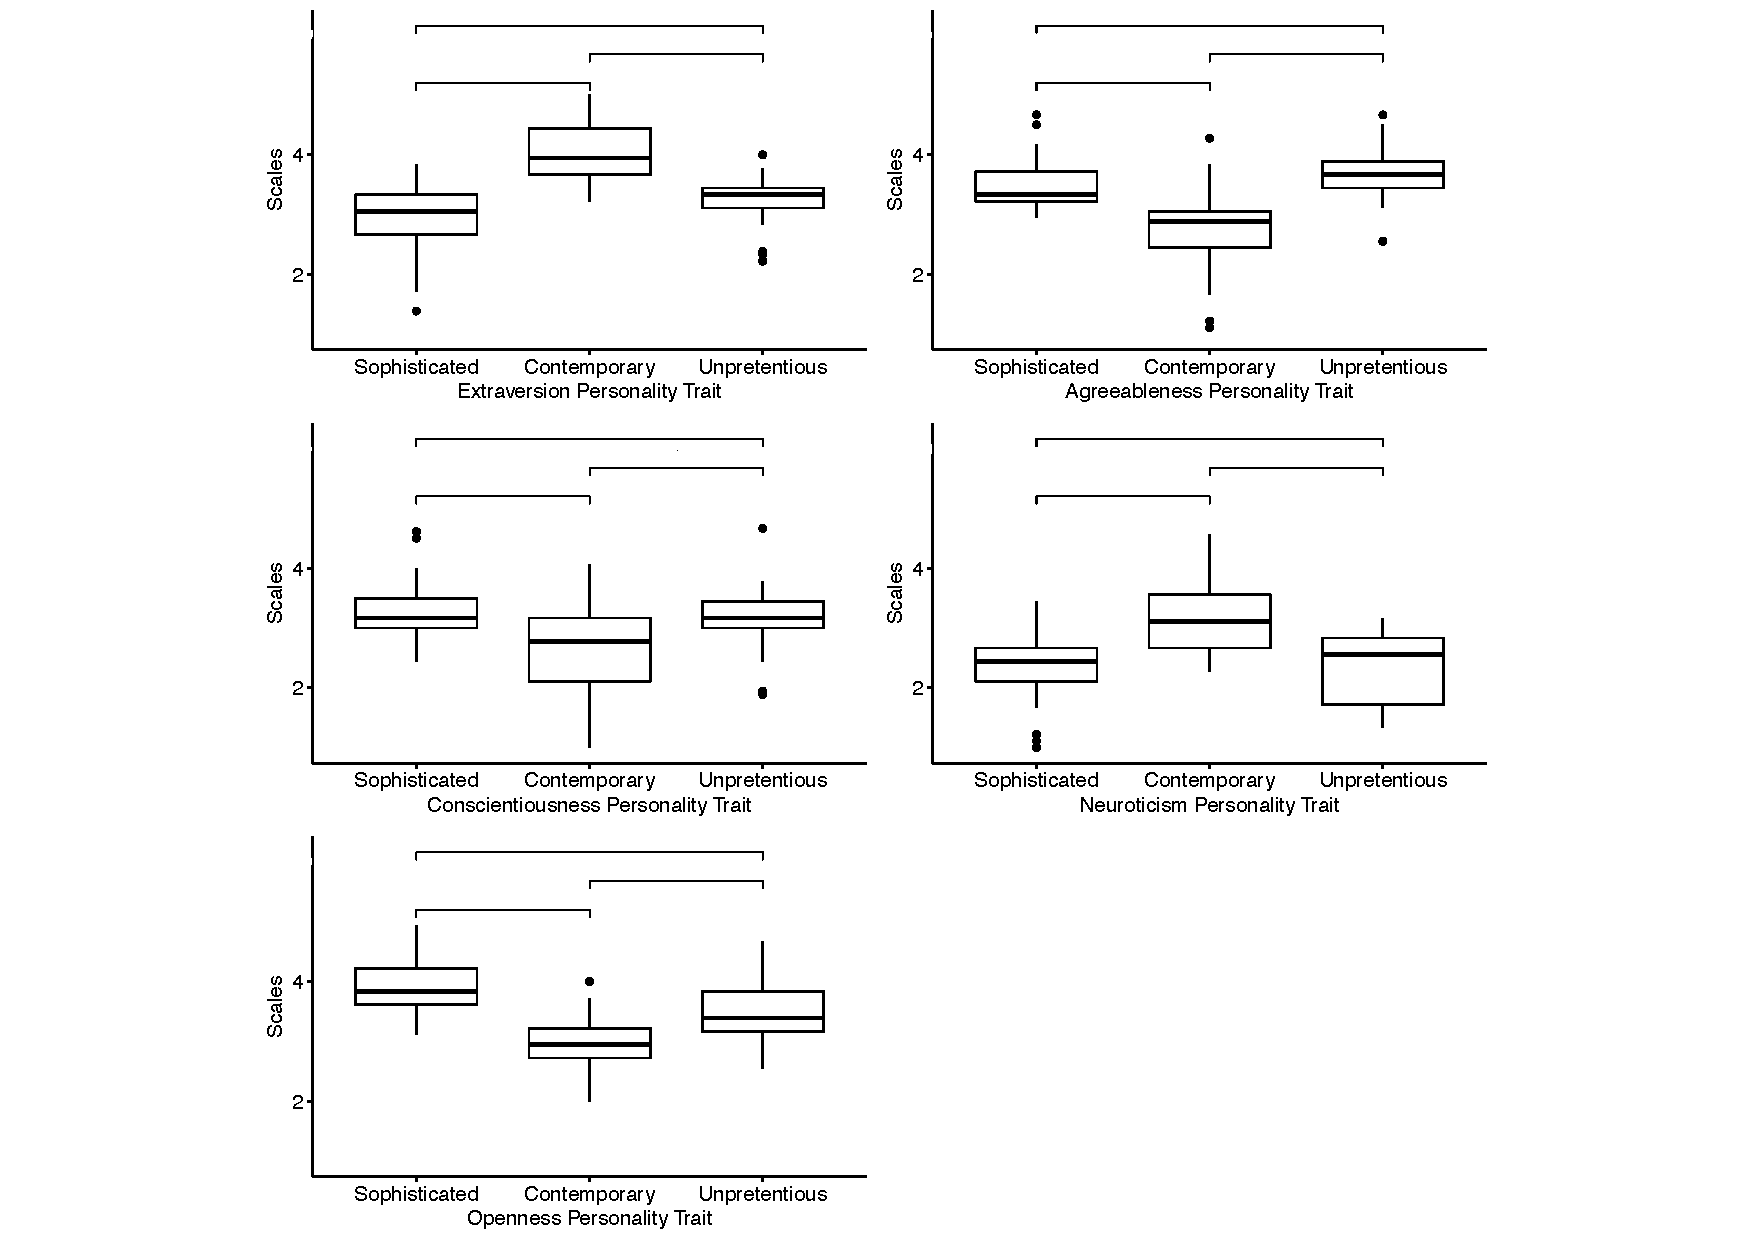
\includegraphics[scale=0.55]{Study1(M-S).pdf}
    \caption{A boxplot for Mascot-Lamp interaction in Study-1}
    \label{fig:MS1}
\end{figure}

%%%%%%%%%%%%%%%%%%%%%%%%%%%%%%%%%%%%%%%%%%%%%%%%%%%%%%%%%%%%%%%%%%%
\subsection{Analysis of within music category study}
\label{subsec:MSstudy2}
In this study, we analyze the effect of each music category, particularly on how each personality
trait is assessed differently within one music condition.

\par\textbf{Sophisticated.}
On average, Sophisticated music has a significant effect on all five personality traits with
p<0.01, df=2 (see Table~\ref{table:friedmanMS2}).
Particularly, this effect is concentrated on Openness personality traits being rated
very high with p<0.01, df=2 (see Table~\ref{table:friedmanMS2}).
When Sophisticated is played, in comparison to all the personality traits, Neuroticism
is rated very low with Med = (see Table~\ref{table:medianMS2}).
Moreover, openness, agreeableness, and neuroticism personality traits shows
significant difference between each other and all other personality traits in the group.

\par\textbf{Contemporary.}
Friedman test shows a significant difference between the ratings of all personality traits and
Contemporary music with p<0.01, df=2 (see Table~\ref{table:friedmanMS2}).
According to the Figure~\ref{fig:MS2}, for Mascot triggering Contemporary music, there is a clear
separation of extraversion samples from all other personality traits with padj<0.01.
The median value for extraversion is very high (Med = 3.9, Max = , Min =) compared to all
other personality traits (Med $\approx$ 3).

\par\textbf{Unpretentious.}
music substantially effected the measurements of all personality traits with
p<0.01, df=4 (see Table~\ref{table:friedmanMS2}).
Based on Wilcoxon tests, neuroticism personality trait is rated very low when Unpretentious music
is played with p < 0.01 (see Figure~\ref{fig:MS2}).
The median values of all other personality traits slightly differ from each other,
condensed around "neutral" rating with Med $\approx$ 3 (see Table~\ref{table:medianMS2})

\begin{longtable}{ |p{2cm}| p{1cm}|p{0.5cm}|p{1.7cm}| }
    \captionsetup{width=13.5cm}
    \caption{The results from Friedman test for all Five Personality traits in case of Mascot-Speakers interaction }
    \label{table:friedmanMS2} \\
    \hline
    \multicolumn{1}{| c}{\textbf{Personality trait }}
    & \multicolumn{1}{| c}{\textbf{$\chi^2$}}
    & \multicolumn{1}{| c}{\textbf{df}}
    & \multicolumn{1}{| c |}{\textbf{p}}  \\
    \hline
    \endfirsthead
    \multicolumn{4}{c}%
    {\tablename\ \thetable\ -- \textit{Continued from previous page}} \\
    \hline
    \multicolumn{1}{| c}{\textbf{Personality trait }}
    & \multicolumn{1}{| c}{\textbf{$\chi^2$}}
    & \multicolumn{1}{| c}{\textbf{df}}
    & \multicolumn{1}{| c |}{\textbf{p}}  \\
    \hline
    \endhead
    \hline \multicolumn{4}{r}{\textit{Continued on next page}} \\
    \endfoot
    \hline
    \endlastfoot
    Sophisticated		&66.573	&4	&p<0.01 \\
    Contemporary		&44.395	&4	&p<0.01\\
    Unpretentious		&57.433	&4	&p<0.01 \\
    \hline
\end{longtable}

\begin{table}[H]
    \renewcommand{\arraystretch}{1.2}
    \caption{Some Caption Y is yellow, O is orange \ldots}
    \label{table:medianMS2}
    \begin{center}
        \begin{tabular}{p{0.05\textwidth}|
        p{0.025\textwidth}|p{0.025\textwidth}|p{0.025\textwidth}|p{0.025\textwidth}|p{0.025\textwidth}||
        p{0.025\textwidth}|p{0.025\textwidth}|p{0.025\textwidth}|p{0.025\textwidth}|p{0.025\textwidth}||
        p{0.025\textwidth}|p{0.025\textwidth}|p{0.025\textwidth}|p{0.025\textwidth}|p{0.025\textwidth}|}
            \cline{2-16}
            & \multicolumn{5}{c||}{\textbf{Sophisticated}} & \multicolumn{5}{c||}{\textbf{Contemporary}}
            & \multicolumn{5}{c|}{\textbf{Unpretentious}} \\
            \cline{2-16}
            & E & A & C & N & O 			    & E & A & C & N & O   	 	& E & A & C & N & O     \\
            \cline{2-16}
            \textbf{Min}  	& 1.4 & 2.9 & 2.4 & 1.0 & 3.1 		& 3.2 & 1.1 & 1.0 & 2.3 & 2.0  	& 2.2 & 2.5 & 1.9 & 1.3 & 2.5  \\
            \textbf{Med} 	& 3.0 & 3.3 & 3.2 & 2.4 & 3.8 		& 3.9 & 2.9 & 2.8 & 3.1 & 2.9  	& 3.3 & 3.7 & 3.2 & 2.5 & 3.4   \\
            \textbf{Max}	& 3.8 & 4.7 & 4.6 & 3.4 & 4.9 		& 5.0 & 4.3 & 4.0 & 4.5 & 4.0  	& 4.0 & 4.7 & 4.7 & 3.2 & 4.7 \\
            \cline{2-16}
        \end{tabular}
    \end{center}
\end{table}

\begin{figure}[H]
    \centering
    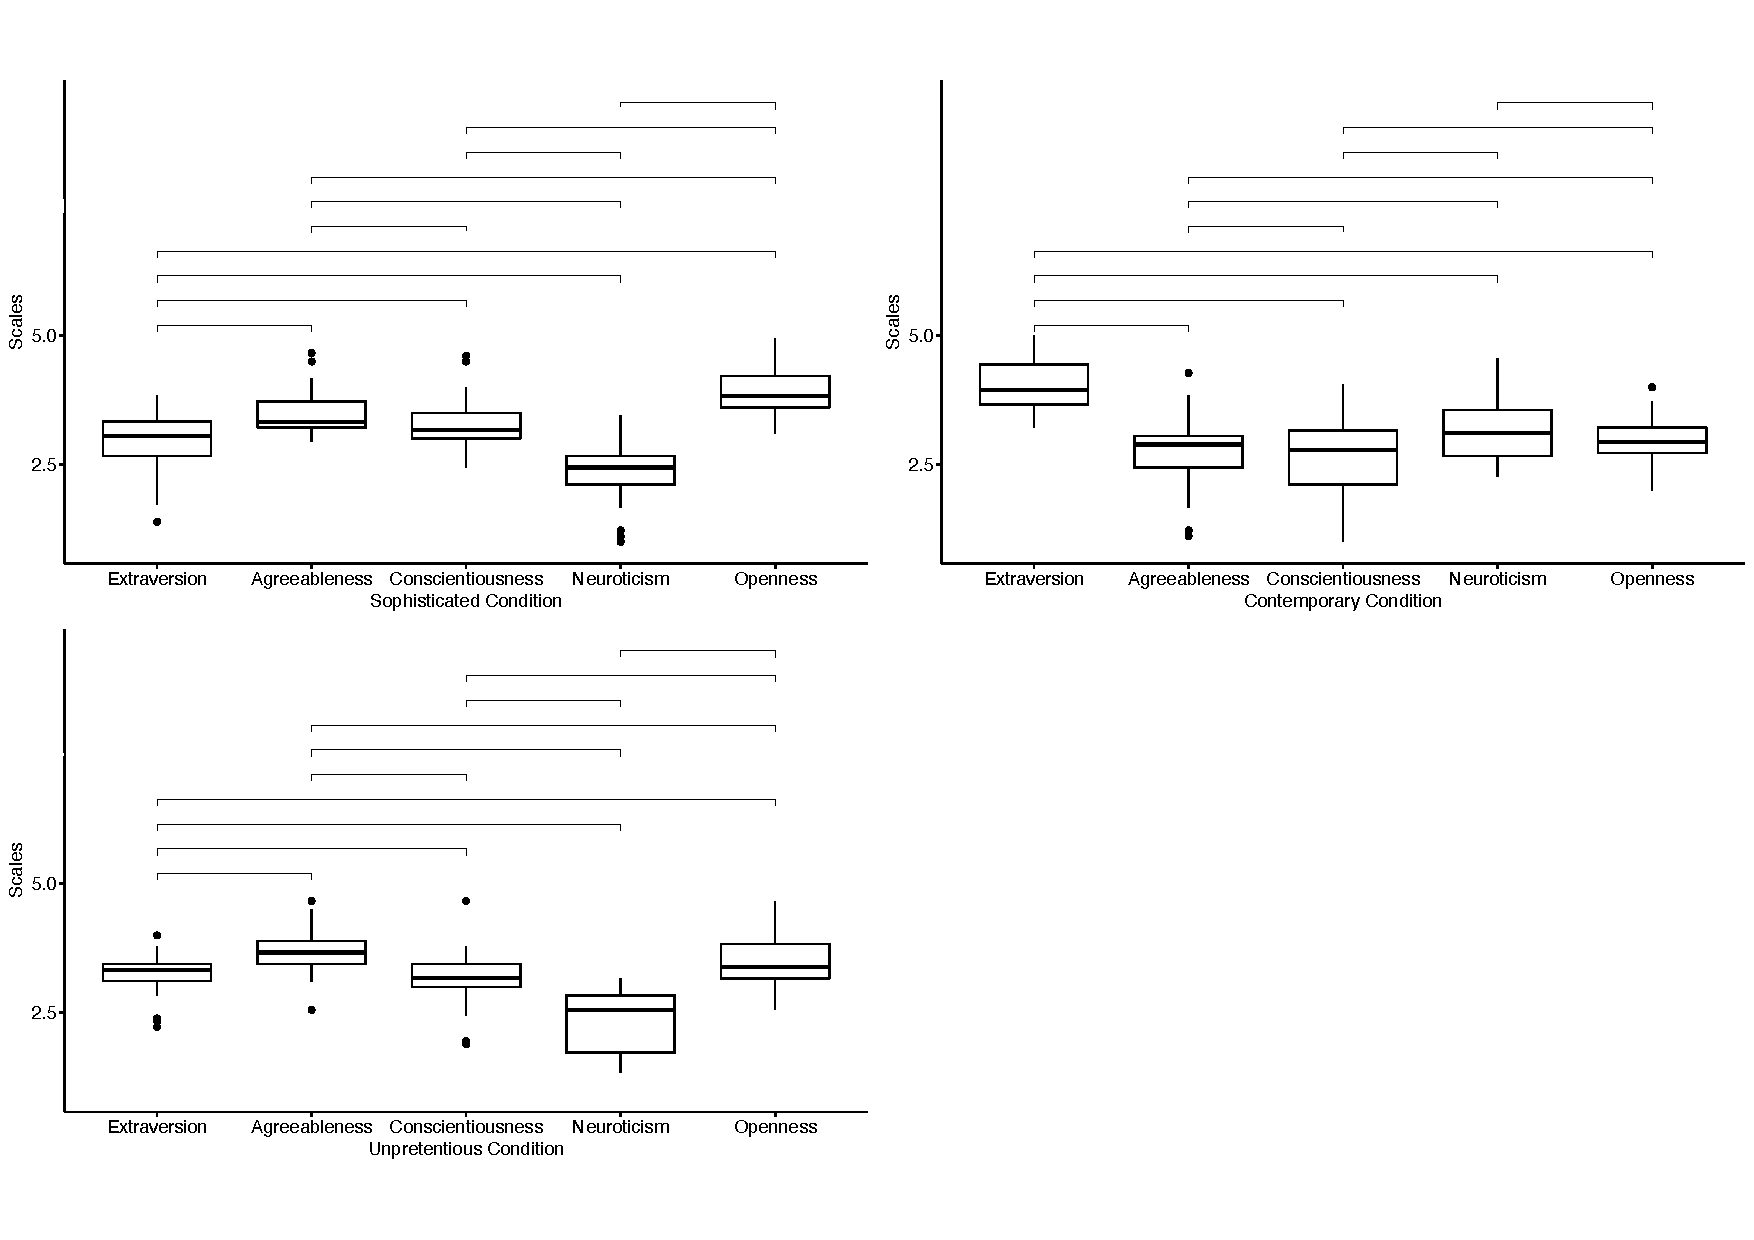
\includegraphics[scale=0.45]{Study2(M-S).pdf}
    \caption{A boxplot for Mascot-Lamp interaction in Study-1}
    \label{fig:MS2}
\end{figure}

%%%%%%%%%%%%%%%%%%%%%%%%%%%%%%%%%%%%%%%%%%%%%%%%%%%%%%%%%%%%%%%%%%%%%%%%%%%%%%%%%%%%%%%%%%%%%%%%%%%%%%%%%%%%%%%%%%%%%%%%
\section{Analysis of Mascot-Mascot interaction}
\label{sec:m-m}
This section covers the analysis of the effect of each level of vibration on the perception
of the personality trait of approaching mascot which triggers this vibration.
The factors that we compare for Mascot-Mascot interaction are five levels of vibration
with a different duration starting from 100 to 500 milliseconds per time.
In Subsection~\ref{subsec:MMstudy1}, we conduct statistical tests for within each
personality trait and in Subsection~\ref{subsec:MMstudy2} for within each vibration level.
In addition, from now on each vibration level is abbreviated accordingly.
For example, the vibration with 500-millisecond duration is abbreviated
as ‘Level-5’, and with 100-millisecond long as ‘Level-1’ and so on.

%%%%%%%%%%%%%%%%%%%%%%%%%%%%%%%%%%%%%%%%%%%%%%%%%%%%%%%%%%%%%%%%%%%
\subsection{Analysis of within personality trait study}
\label{subsec:MMstudy1}
In the first study, we analyse the impact of all vibration levels within each personality trait.
In this study, we analyze each personality trait individually and explore which vibration
level conveys it most.

\par\textbf{Extraversion.}
Friedman test shows significant difference between all levels of vibration in the
ratings of Extraversion personality trait with p<0.01 (see Table~\ref{table:friedmanMM1}).
In comparison to all other levels, Level5 and Level-4 show a significant difference
in the measurements of the extraversion personality with p<0.05 (see Figure~\ref{fig:MM1}).
Both of these levels were highly scored as the behavior of an extravert mascot
with Med = 4.0, for Level-5 and Med = 3.0 for Level-4 (see Table~\ref{table:medianMM1}).

\par\textbf{Agreeableness.}
All vibration levels substantially effected the measurements of Agreeableness personality
trait with p<0.01, df=4 (see Table~\ref{table:friedmanMM1}).

Both Level-2 and Level-3 revealed a significant effect for mascot being
assessed as agreeable with padj < 0.05 (see Figure~\ref{fig:MM1}).
Overall, the majority of votes given for Level-2 (Med = 4.0, Max = , Min = ) and Level-3
(Med = 3.5, Max = , Min = ) attributing agreeableness personality, are higher than most
votes given for other vibration levels (see Table~\ref{table:medianMM1}).

\par\textbf{Conscientiousness.}
There is a significant impact of all vibration levels on the assessment of conscientiousness
personality trait with p<0.01, df=4 (see Table~\ref{table:friedmanMM1}).
The analysis revealed strong impact of levels three abd four on padj < 0.01 (see Figure~\ref{fig:MM1}).
Moreover, the median values for Level-3 (Med = 3.8) and Level-4 (Med = 4.0) are high enough
to show strong impact of these levels to measure mascot as Conscientious (see Table~\ref{table:medianMM1}).

\par\textbf{Neuroticism.}
There is a significant difference of measurements of each level of vibration within Neuroticism
personality trait with p<0.01, df=4 (see Table~\ref{table:friedmanMM1}).
Moreover, especially this difference is concentrated on the ratings for Level-1 with Med = 3.7
in comparison to other levels with Med < 2.5 (see Table~\ref{table:medianMM1}).
For a Neuroticism personality trait, there is a good separation of samples for Level-1
from all other vibration levels with p<0.05 (see Figure~\ref{fig:MM1}).

\par\textbf{Openness.}
Table~\ref{table:friedmanMM1} reveals a difference between all five vibration levels within
openness personality trait with p<0.05, df=4 (see Table~\ref{table:friedmanMM1}).

The Wilcoxon test revealed a significant difference between levels one and two, on
openness personality trait with p < 0.05 (see Figure~\ref{fig:MM1}).
The median values for Level-5, Level4, Level-2, and Level-1 imply the overall
similarity of votes concentrated on the “neutral” scale with Med<2.7 (see Table~\ref{table:medianMM1}).

\begin{longtable}{ |p{3cm}| p{1cm}|p{0.5cm}|p{1.7cm}| }
    \captionsetup{width=13.5cm}
    \caption{The results from Friedman test for all Five Personality traits in case of Mascot-Mascot interaction }
    \label{table:friedmanMM1} \\
    \hline
    \multicolumn{1}{| c}{\textbf{Personality trait }}
    & \multicolumn{1}{| c}{\textbf{$\chi^2$}}
    & \multicolumn{1}{| c}{\textbf{df}}
    & \multicolumn{1}{| c |}{\textbf{p}}  \\
    \hline
    \endfirsthead
    \multicolumn{4}{c}%
    {\tablename\ \thetable\ -- \textit{Continued from previous page}} \\
    \hline
    \multicolumn{1}{| c}{\textbf{Personality trait }}
    & \multicolumn{1}{| c}{\textbf{$\chi^2$}}
    & \multicolumn{1}{| c}{\textbf{df}}
    & \multicolumn{1}{| c |}{\textbf{p}}  \\
    \hline
    \endhead
    \hline \multicolumn{4}{r}{\textit{Continued on next page}} \\
    \endfoot
    \hline
    \endlastfoot
    Extraversion		&30.82	&4	&p<0.01 \\
    Agreeableness		&19.767	&4	&p<0.01 \\
    Conscientiousness	& 43.236	&4	&p<0.01 \\
    Neuroticism		&28.212	&4	&p<0.01\\
    Openness			&11.169	&4	&p<0.05 \\
    \hline
\end{longtable}

\begin{table}[H]
    \renewcommand{\arraystretch}{1.2}
    \caption{Some Caption Y is yellow, O is orange \ldots}
    \label{table:medianMM1}
    \begin{center}
        \begin{tabular}{p{0.05\textwidth}|
        p{0.025\textwidth}|p{0.025\textwidth}|p{0.025\textwidth}|p{0.025\textwidth}|p{0.025\textwidth}||
        p{0.025\textwidth}|p{0.025\textwidth}|p{0.025\textwidth}|p{0.025\textwidth}|p{0.025\textwidth}||
        p{0.025\textwidth}|p{0.025\textwidth}|p{0.025\textwidth}|p{0.025\textwidth}|p{0.025\textwidth}|}
            \cline{2-16}
            & \multicolumn{5}{c||}{\textbf{Extraversion}} & \multicolumn{5}{c||}{\textbf{Agreeableness}}
            & \multicolumn{5}{c|}{\textbf{Conscientiousness}} \\
            \cline{2-16}
            & L-1 & L-2 & L-3 & L-4 & L-5 			    & L-1 & L-2 & L-3 & L-4 & L-5   	 	& L-1 & L-2 & L-3 & L-4 & L-5      \\
            \cline{2-16}
            \textbf{Min}  	& 1.2 & 1.7 & 1.3 & 2.2 & 2.3 		& 1.7 & 2.0 & 2.5 & 1.3 & 1.3  	& 1.7 & 1.5 & 2.8 & 2.2 & 1.7  \\
            \textbf{Med} 	& 2.0 & 2.0 & 2.7 & 3.0 & 4.0 		& 2.5 & 4.0 & 3.5 & 2.8 & 2.7  	& 2.5 & 2.7 & 3.8 & 4.0 & 2.8  \\
            \textbf{Max}	& 3.8 & 4.0 & 4.3 & 4.7 & 4.7 		& 4.0 & 4.7 & 5.0 & 4.0 & 3.8  	& 3.8 & 4.2 & 5.0 & 5.0 & 3.8 \\
            \cline{2-16}
            \cline{2-11}
            &  \multicolumn{5}{|c||}{\textbf{Neuroticism}} & \multicolumn{5}{|c||}{\textbf{Openness}} \\
            \cline{2-11}
            & L-1 & L-2 & L-3 & L-4 & L-5  			& L-1 & L-2 & L-3 & L-4 & L-5     		\\
            \cline{2-11}
            \textbf{Min} 	& 2.0 & 1.3 & 1.3 & 1.0 & 1.0 		& 1.1 & 1.8 & 1.5 & 1.0 & 1.3 	\\
            \textbf{Med}    & 3.7 & 2.1 & 1.8 & 2.2 & 2.3 	    & 2.3 & 2.5 & 3.3 & 2.7 & 2.7 	\\
            \textbf{Max}  	& 4.7 & 3.7 & 4.2 & 3.5 & 3.3 		& 4.2 & 4.5 & 4.3 & 4.5 & 4.0  	\\
            \cline{2-11}
        \end{tabular}
    \end{center}
\end{table}

\begin{figure}[H]
    \centering
    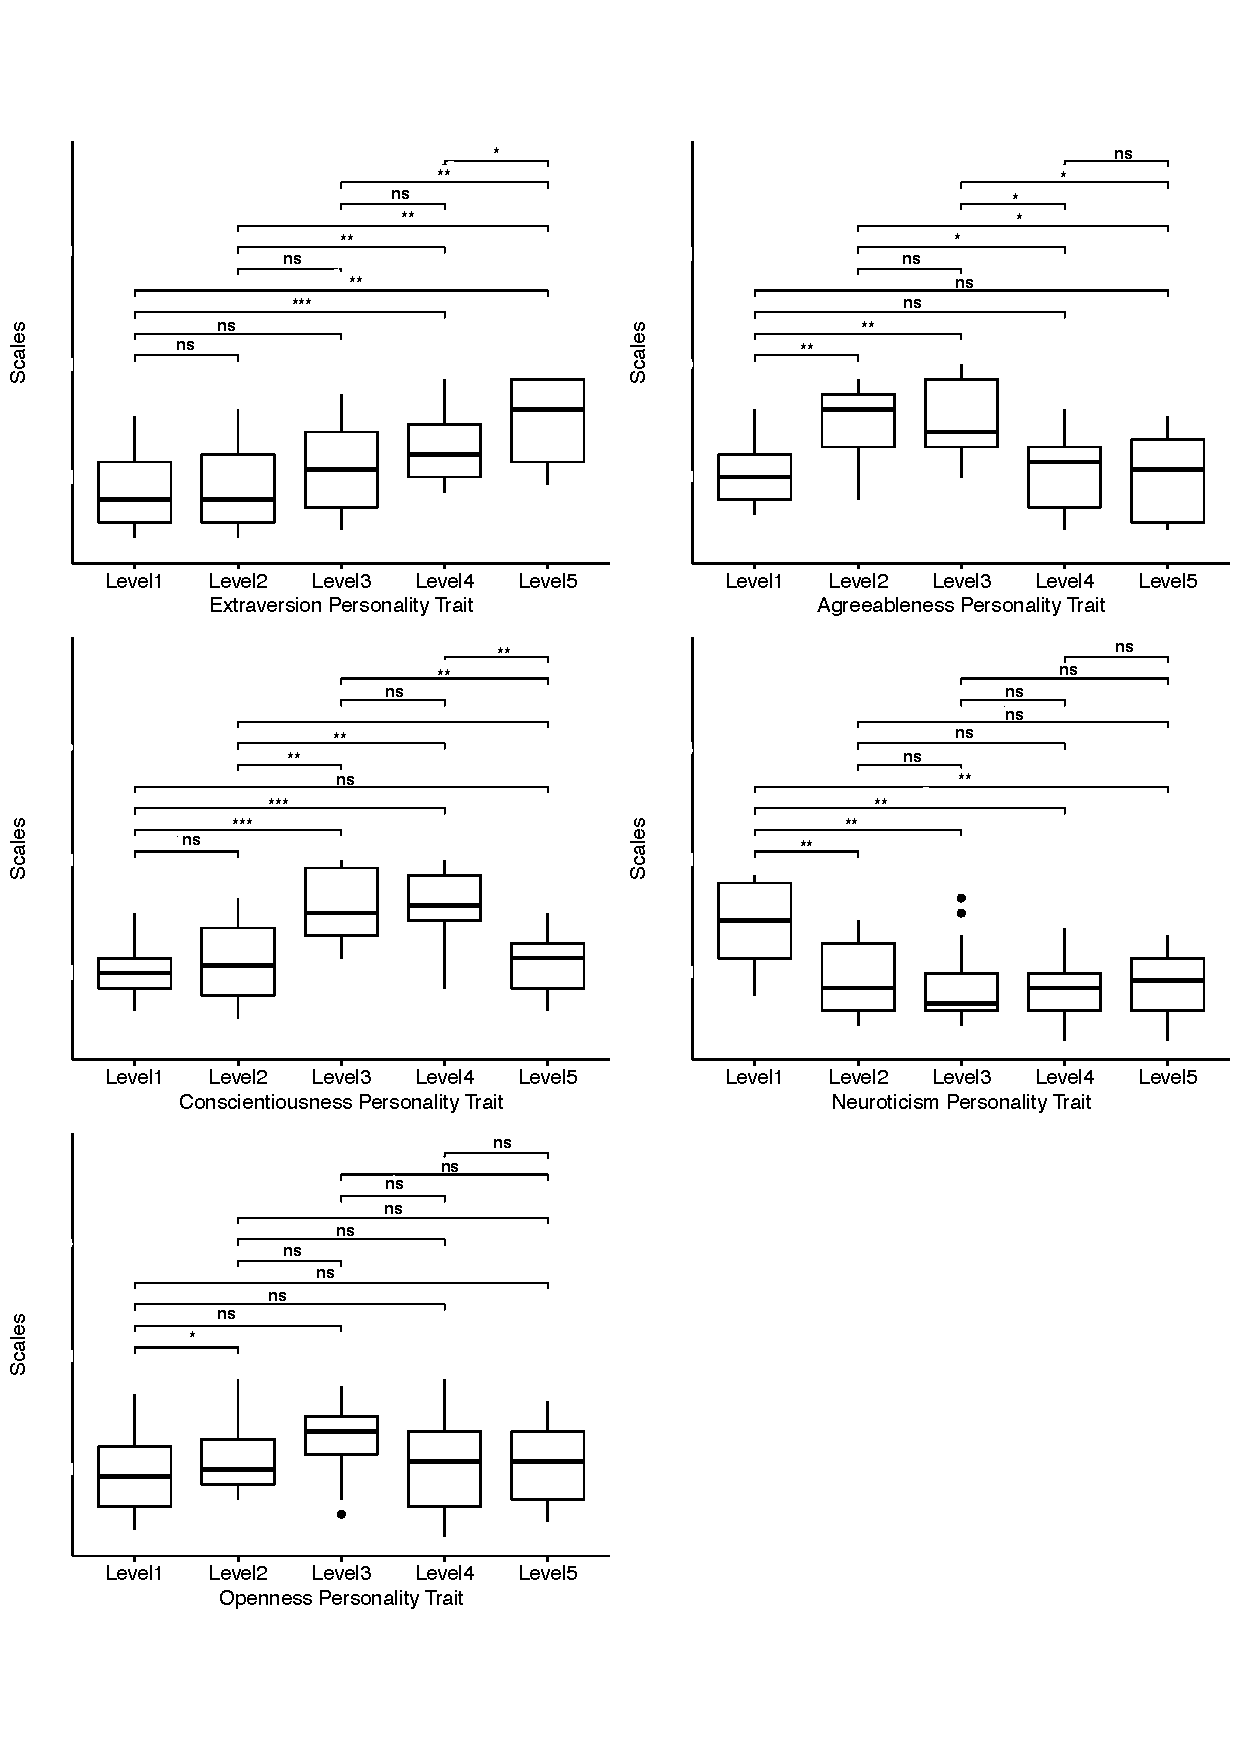
\includegraphics[scale=0.55]{Study1(M-M).pdf}
    \caption{A boxplot for Mascot-Lamp interaction in Study-1}
    \label{fig:MM1}
\end{figure}

%%%%%%%%%%%%%%%%%%%%%%%%%%%%%%%%%%%%%%%%%%%%%%%%%%%%%%%%%%%%%%%%%%%
\subsection{Analysis of within vibration level study}
\label{subsec:MMstudy2}
The second study analyzes each vibration level individually and the difference
of each personality trait within a specific vibration level.

\par\textbf{Level-1.}
Friedman test shows a significant difference between the ratings of all personality traits
and vibration Level-1 with p<0.01, df=4 (see Table~\ref{table:friedmanMM2}).
This difference especially is concentrated on Neuroticism which distinguished it from all
other personality traits with padj<0.05 (see Figure~\ref{fig:}).
In comparison to Neuroticism (Med = 3.7), the median rates given for extraversion,
agreeableness, conscientiousness and openness personality traits are relatively similar,
namely 2.0, 2.5, 2.5, 2.3 respectively (see Table~\ref{table:medianMM2}).

\par\textbf{Level-2.}
On average, Level-2 has a significant effect on the ratings of all five personality
traits with p<0.01, df=4 (see Table~\ref{table:friedmanMM2}).
Based on Wilcoxon tests, there are four groups of personality trait being effected by
vibration Level-2 with padj<0.05 (see Figure~\ref{fig:MM2}).
Moreover, agreeableness is the most distinguishable with being rated higher
than all other personality traits.

\par\textbf{Level-3.}
has a substantial impact on the measurements of personality trait
with p<0.01, df=4 (see Table~\ref{table:friedmanMM2}).
Level-3 effects the ratings of two personality traits: agreeableness and
conscientiousness with padj< 0.05 (see Figure~\ref{fig:MM2}).

\par\textbf{Level-4.}
There is a statistically significant difference between personality trait measurements
with Level-4 with p<0.01, df=4 (see Table~\ref{table:friedmanMM2}).
Level-4 has an impact on the ratings of  two personality traits with the highest scores
such as conscientiousness and extraversion
with a very significant p < 0.01.

\par\textbf{Level-5.}
Overall, all personality traits shows different results when each mascot vibrating 500 milliseconds
per time (i.e Level-5) with p<0.01, df=4 (see Table~\ref{table:friedmanMM2}).
Level-5 distinguishes Exraversion from all other personality traits having the
highest ratings with padj<0.05 (see Figure~\ref{fig:MM2}).
The median values for all other personality traits are lower than neutral scale (Med < 3.0)
in comparison to neuroticism with Med = 4.0 (see Table~\ref{table:medianMM2}).

\begin{longtable}{ |p{2cm}| p{1cm}|p{0.5cm}|p{1.7cm}| }
    \captionsetup{width=13.5cm}
    \caption{The results from Friedman test for all Five Personality traits in case of Mascot-Mascot interaction}
    \label{table:friedmanMM2} \\
    \hline
    \multicolumn{1}{| c}{\textbf{Personality trait }}
    & \multicolumn{1}{| c}{\textbf{$\chi^2$}}
    & \multicolumn{1}{| c}{\textbf{df}}
    & \multicolumn{1}{| c |}{\textbf{p}}  \\
    \hline
    \endfirsthead
    \multicolumn{4}{c}%
    {\tablename\ \thetable\ -- \textit{Continued from previous page}} \\
    \hline
    \multicolumn{1}{| c}{\textbf{Personality trait }}
    & \multicolumn{1}{| c}{\textbf{$\chi^2$}}
    & \multicolumn{1}{| c}{\textbf{df}}
    & \multicolumn{1}{| c |}{\textbf{p}}  \\
    \hline
    \endhead
    \hline \multicolumn{4}{r}{\textit{Continued on next page}} \\
    \endfoot
    \hline
    \endlastfoot
    Level-1		&24.008	&4	&p<0.01 \\
    Level-2		&24.525	&4	&p<0.01 \\
    Level-3		&35.165	&4	&p<0.01 \\
    Level-4		&46.603	&4	&p<0.01 \\
    Level-5		&24.1	&4	&p<0.01 \\
    \hline
\end{longtable}

\begin{table}[H]
    \renewcommand{\arraystretch}{1.2}
    \caption{Some Caption Y is yellow, O is orange \ldots}
    \label{table:medianMM2}
    \begin{center}
        \begin{tabular}{p{0.05\textwidth}|
        p{0.025\textwidth}|p{0.025\textwidth}|p{0.025\textwidth}|p{0.025\textwidth}|p{0.025\textwidth}||
        p{0.025\textwidth}|p{0.025\textwidth}|p{0.025\textwidth}|p{0.025\textwidth}|p{0.025\textwidth}||
        p{0.025\textwidth}|p{0.025\textwidth}|p{0.025\textwidth}|p{0.025\textwidth}|p{0.025\textwidth}|}
            \cline{2-16}
            & \multicolumn{5}{c||}{\textbf{Level-1}} & \multicolumn{5}{c||}{\textbf{Level-2}}
            & \multicolumn{5}{c|}{\textbf{Level-3}} \\
            \cline{2-16}
            & E & A & C & N & O  			    & E & A & C & N & O   	 	& E & A & C & N & O      \\
            \cline{2-16}
            \textbf{Min}  	& 1.2 & 1.7 & 1.7 & 2.0 & 1.2 		& 1.2 & 2.0 & 1.5 & 1.3 & 1.8  	& 1.3 & 2.5 & 2.8 & 1.3 & 1.5  \\
            \textbf{Med} 	& 2.0 & 2.5 & 2.5 & 3.7 & 2.3 		& 2.0 & 4.0 & 2.7 & 2.2 & 2.5  	& 2.7 & 3.5 & 3.8 & 1.8 & 3.3  \\
            \textbf{Max}	& 3.8 & 4.0 & 3.8 & 4.7 & 4.2 		& 4.0 & 4.7 & 4.2 & 3.7 & 4.5  	& 4.3 & 5.0 & 5.0 & 4.2 & 4.3 \\
            \cline{2-16}
            \cline{2-11}
            &  \multicolumn{5}{|c||}{\textbf{Level-4}} & \multicolumn{5}{|c||}{\textbf{Level-5}} \\
            \cline{2-11}
            & E & A & C & N & O  			& E & A & C & N & O     		\\
            \cline{2-11}
            \textbf{Min} 	& 2.2 & 1.3 & 2.2 & 1.0 & 1.0 		& 2.3 & 1.3 & 1.7 & 1.0 & 1.3 	\\
            \textbf{Med}    & 3.0 & 2.8 & 4.0 & 2.2 & 2.7 	    & 4.0 & 2.7 & 2.8 & 2.3 & 2.7 	\\
            \textbf{Max}  	& 4.7 & 4.0 & 5.0 & 3.5 & 4.5 		& 4.7 & 3.8 & 3.8 & 3.3 & 4.0  	\\
            \cline{2-11}
        \end{tabular}
    \end{center}
\end{table}

\begin{figure}[H]
    \centering
    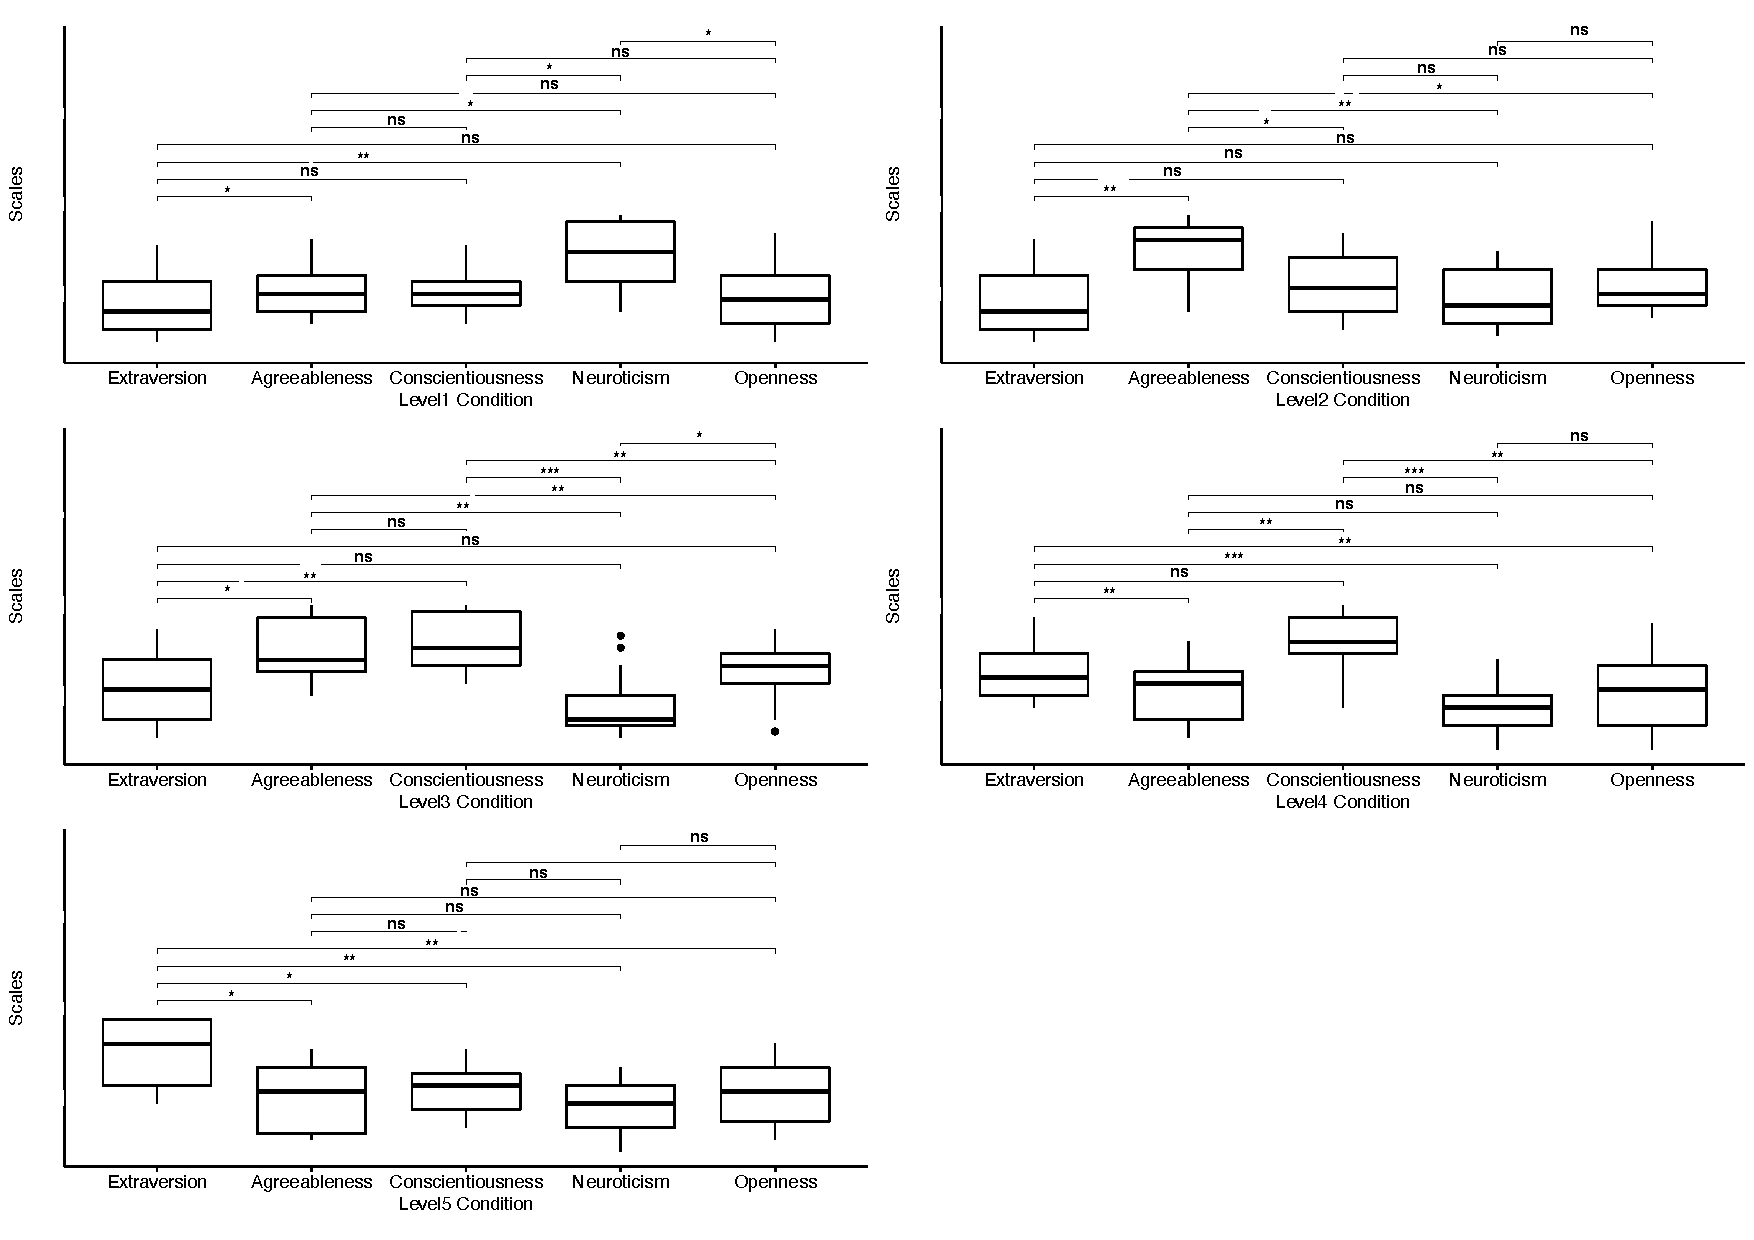
\includegraphics[scale=0.45]{Study2(M-M).pdf}
    \caption{A boxplot for Mascot-Lamp interaction in Study-1}
    \label{fig:MM2}
\end{figure}

%%%%%%%%%%%%%%%%%%%%%%%%%%%%%%%%%%%%%%%%%%%%%%%%%%%%%%%%%%%%%%%%%%%%%%%%%%%%%%%%%%%%%%%%%%%%%%%%%%%%%%%%%%%%%%%%%%%%%%%%
\section{Analysis of Mascot-Tablet interaction}
\label{sec:m-t}
The section describes the impact of the screen color of a tablet on the assessment of the personality trait that
mascot was assigned.
The factors that we compare for Mascot-Tablet interaction are yellow,
orange, turquoise, blood-red and pink screen colors.
Subsection~\ref{subsec:MTstudy1} shows the analysis of within personality study and Subsection~\ref{subsec:MTstudy2} of condition study (i.e color)

%%%%%%%%%%%%%%%%%%%%%%%%%%%%%%%%%%%%%%%%%%%%%%%%%%%%%%%%%%%%%%%%%%%
\subsection{Analysis of within personality trait study}
\label{subsec:MTstudy1}
In our first study, we focus on each personality by comparing the scores given
for each color within that personality trait.

\par\textbf{Extraversion.}
For the measurements of extraversion personality,
the most significant difference was observed when comparing yellow, orange with
blood-red, pink colors with padj<0.05.
Meaning that colors with padj<0.05 shows that samples from yellow and orange colors are separated
from blood-red and pink samples (see Figure~\ref{fig:MT1}).
Moreover, in comparison to other colors most samples for orange are concentrated around
an “accurate” score (Med = 4.2, Max = 5.0) (see Table~\ref{table:medianMT1}).

\par\textbf{Agreeableness.}
Change in tablet's screen color significantly influenced the participants' ratings of
Agreeableness personality trait with p<0.01, df=4 (see Table~\ref{table:friedmanMT1}).
Figure~\ref{fig:MT1}) shows a good separation of turquoise and pink colors
from all others implying that there is a difference in ratings the
agreeableness personality traits having padj < 0.01.
However, there is no strong difference between turquoise and pink colors with
the same value Med = 3.7 (see Table~\ref{table:medianMT1}).

\par\textbf{Conscientiousness.}
There is a significant difference in the rating of Conscientiousness personality trait
when comparing screen colors with p<0.01, df=4 (see Table~\ref{table:friedmanMT1}).
According to Figure~\ref{fig:MT1}, there is a significant difference for
tablet displaying turquoise color in rating mascot as conscientiousness with padj < 0.05.
The median values for yellow (Med = 2.7), pink (Med = 2.8) and orange (Med = 2.7) colors are
concentrated around the “neutral” scale, whereas turquoise (Med = 4.2) (see Table~\ref{table:medianMT1}).

\par\textbf{Neuroticism.}
All predefined screen colors substantially effected the measurements of Neuroticism personality
trait with p<0.01, df=4 (see Table~\ref{table:friedmanMT1}).
According to Figure~\ref{fig:MT1}, there is a great separation of blood-red
samples from all other screen colors.
Moreover, there is a significant difference in the rating of Neuroticism when comparing
Blood-red with other screen colors with padj<0.05.
The rating for blood-red is higher with Med = 3.8 compared to all other colors
being rated low with M $\leq$ 2.5 (see Table~\ref{table:medianMT1}).

\par\textbf{Openness.}
Table~\ref{table:friedmanMT1} shows the different rating based on all colors within openness
personality trait with p<0.01, df=4 (see Table~\ref{table:friedmanMT1}).
According to the Wilcoxon tests, during the measurements of a mascot's 'openness to experience'
personality trait, the yellow is significantly different from all other screen
colors with padj < 0.05 (see Figure~\ref{fig:MT1}).
In comparison to all other colors (M $\leq$ 3.0), most of the samples of yellow color are discriminated
from all others concentrating around an “accurate” scale with a Med = 4.0 (see Table~\ref{table:medianMT1}).

\begin{longtable}{ |p{2.7cm}| p{1cm}|p{0.5cm}|p{1.7cm}| }
    \captionsetup{width=13.5cm}
    \caption{The results from Friedman test for all Five Personality traits in case of Mascot-Tablet interaction}
    \label{table:friedmanMT1} \\
    \hline
    \multicolumn{1}{| c}{\textbf{Personality trait }}
    & \multicolumn{1}{| c}{\textbf{$\chi^2$}}
    & \multicolumn{1}{| c}{\textbf{df}}
    & \multicolumn{1}{| c |}{\textbf{p}}  \\
    \hline
    \endfirsthead
    \multicolumn{4}{c}%
    {\tablename\ \thetable\ -- \textit{Continued from previous page}} \\
    \hline
    \multicolumn{1}{| c}{\textbf{Personality trait }}
    & \multicolumn{1}{| c}{\textbf{$\chi^2$}}
    & \multicolumn{1}{| c}{\textbf{df}}
    & \multicolumn{1}{| c |}{\textbf{p}}  \\
    \hline
    \endhead
    \hline \multicolumn{4}{r}{\textit{Continued on next page}} \\
    \endfoot
    \hline
    \endlastfoot
    Extraversion		&28.841	&4	&p<0.01 \\
    Agreeableness		&52.895	&4	&p<0.01 \\
    Conscientiousness	&32.891	&4	&p<0.01 \\
    Neuroticism		&30.466	&4	&p<0.01 \\
    Openness			&37.725	&4	&p<0.01 \\
    \hline
\end{longtable}

\begin{table}[H]
    \renewcommand{\arraystretch}{1.2}
    \caption{Some Caption Y is yellow, O is orange \ldots}
    \label{table:medianMT1}
    \begin{center}
        \begin{tabular}{p{0.05\textwidth}|
        p{0.025\textwidth}|p{0.025\textwidth}|p{0.025\textwidth}|p{0.025\textwidth}|p{0.025\textwidth}||
        p{0.025\textwidth}|p{0.025\textwidth}|p{0.025\textwidth}|p{0.025\textwidth}|p{0.025\textwidth}||
        p{0.025\textwidth}|p{0.025\textwidth}|p{0.025\textwidth}|p{0.025\textwidth}|p{0.025\textwidth}|}
            \cline{2-16}
            & \multicolumn{5}{c||}{\textbf{Extraversion}} & \multicolumn{5}{c||}{\textbf{Agreeableness}}
            & \multicolumn{5}{c|}{\textbf{Conscientiousness}} \\
            \cline{2-16}
            & Y & O & T & B & P 			    & Y & O & T & B & P  	 	& Y & O & T & B & P     \\
            \cline{2-16}
            \textbf{Min}  	& 2.0 & 1.7 & 2.0 & 1.2 & 1.7 		& 1.5 & 1.2 & 1.8 & 1.0 & 1.7  	& 1.8 & 2.2 & 2.0 & 1.0 & 2.0  \\
            \textbf{Med} 	& 3.3 & 4.2 & 2.8 & 1.7 & 2.5 		& 3.0 & 2.3 & 3.7 & 1.8 & 3.7  	& 2.7 & 2.7 & 4.2 & 2.3 & 2.8  \\
            \textbf{Max}	& 4.0 & 5.0 & 4.3 & 4.7 & 3.8 		& 3.7 & 4.5 & 4.2 & 3.3 & 5.0  	& 3.5 & 4.5 & 5.0 & 4.3 & 4.7 \\
            \cline{2-16}
            \cline{2-11}
            &  \multicolumn{5}{|c||}{\textbf{Neuroticism}} & \multicolumn{5}{|c||}{\textbf{Openness}} \\
            \cline{2-11}
            & Y & O & T & B & P 			& Y & O & T & B & P    		\\
            \cline{2-11}
            \textbf{Min} 	& 1.3 & 1.5 & 1.0 & 1.5 & 1.2 		& 2.5 & 1.3 & 2.0 & 1.0 & 1.5 	\\
            \textbf{Med}    & 2.2 & 2.5 & 2.5 & 3.8 & 2.3 	    & 4.0 & 3.0 & 3.0 & 2.7 & 2.7 	\\
            \textbf{Max}  	& 3.7 & 4.3 & 3.5 & 5.0 & 4.2 		& 5.0 & 5.0 & 4.2 & 3.8 & 3.8  	\\
            \cline{2-11}
        \end{tabular}
    \end{center}
\end{table}

\begin{figure}[H]
    \centering
    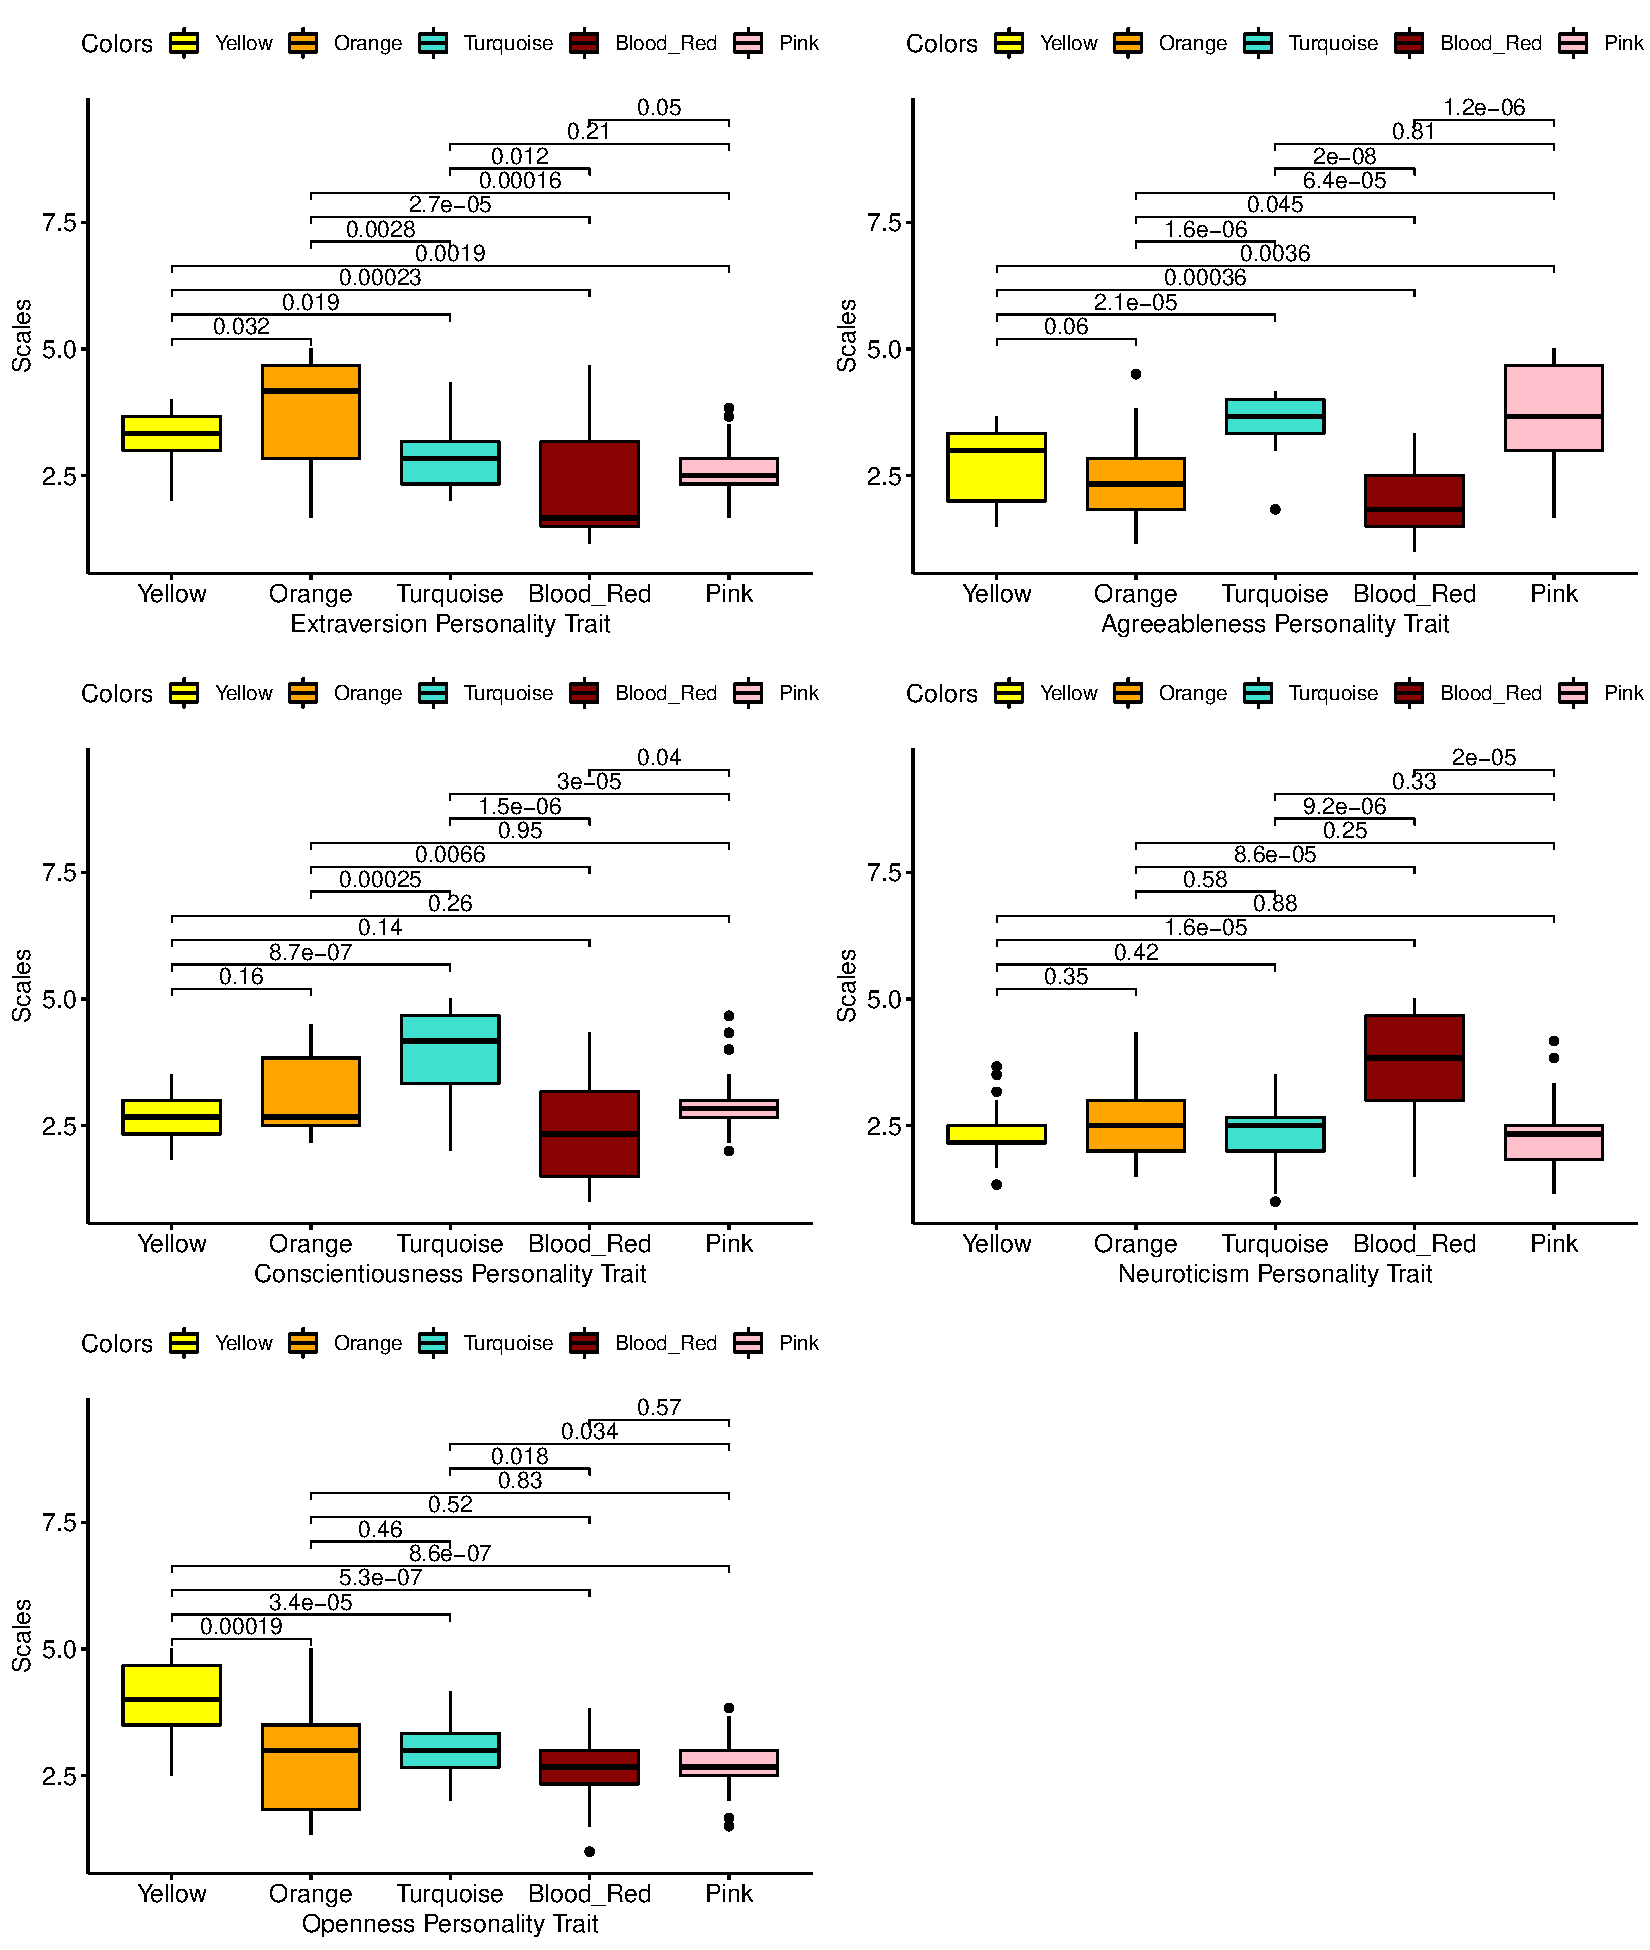
\includegraphics[scale=0.55]{Study1(M-T).pdf}
    \caption{A boxplot for Mascot-Lamp interaction in Study-1}
    \label{fig:MT1}
\end{figure}

\par\textbf{Extraversion.}

%%%%%%%%%%%%%%%%%%%%%%%%%%%%%%%%%%%%%%%%%%%%%%%%%%%%%%%%%%%%%%%%%%%
\subsection{Analysis of within screen color study}
\label{subsec:MTstudy2}
For the second study, we focus on each color by comparing the different measurements of five
personality traits within each screen color.

\par\textbf{Yellow.}
Friedman test showed a significant difference of the ratings each personality trait
within yellow lighting color with p<0.01, df=4 (see Table~\ref{table:friedmanMT2}).
When Mascot trigger yellow background color, tests reveals the difference concentrated on Openness
personality trait which is rated very high with p<0.01 (see Figure~\ref{fig:MT1}).

\par\textbf{Orange.}
There is a statistically substantial difference between personality trait measurements within
orange color with p<0.01, df=4 (see Table~\ref{table:friedmanML2}).
Wilcoxon tests show three groups having significant different ratings when orange
color is triggered.
There are extraversion and agreeableness, extraversion and neuroticism, agreeableness and
conscientiousness personality traits (see Figure~\ref{fig:MT1}).
The extraversion seems to have the highest overall positive opinions
with median = 4.2 (see Appendix A.8)

\par\textbf{Turquoise.}
Overall all personality traits shows different results when light was transformed to turquoise color
with p<0.01, df=4 (see Table~\ref{table:friedmanML2}).
Turquoise screen color shows the distinguishable effects on all personality trait ratings.
Particularly, the measurements of conscientiousness and agreeableness personality traits are the most
conveyed by turquoise colors with a padj< 0.05 (see Table~\ref{fig:MT2}).
Moreover, the median value for conscientiousness (Med = 4.2) is higher than for agreeableness
(Med = 3.7) and all other personality traits (Med $\leq$ 3.0) (see Table~\ref{table:friedmanMT2}).

\par\textbf{Blood-red.}
lighting color reveals significant difference in measurements of all personality traits
with p<0.01, df=4 (see Table~\ref{table:friedmanML2}).
For blood-red color, there is a significant difference in ratings of Neuroticism
being higher that for all other personality traits with p<0.01.
The boxplots show a great separation of neuroticism samples from all
other personality traits (see Figure~\ref{fig:MT1}).


\par\textbf{Pink.}
There is a significant difference in rating Mascots' personality when the pink light is
triggered with p<0.01, df=4 (see Table~\ref{table:friedmanML2}).
There is a significant impact of pink color on agreeableness personality traits with p < 0.05.
However, we could not find any difference in the ratings of pink color when
we compare agreeableness and conscientiousness personality traits (padj>0.05).


\begin{longtable}{ |p{3cm}| p{1.7cm}|p{0.5cm}|p{1.7cm}| }
    \captionsetup{width=13.5cm}
    \caption{The results from Friedman test for all Five Personality traits in case of Mascot-Tablet interaction}
    \label{table:friedmanMT2} \\
    \hline
    \multicolumn{1}{| c}{\textbf{Personality trait }}
    & \multicolumn{1}{| c}{\textbf{$\chi^2$}}
    & \multicolumn{1}{| c}{\textbf{df}}
    & \multicolumn{1}{| c |}{\textbf{p}}  \\
    \hline
    \endfirsthead
    \multicolumn{4}{c}%
    {\tablename\ \thetable\ -- \textit{Continued from previous page}} \\
    \hline
    \multicolumn{1}{| c}{\textbf{Personality trait }}
    & \multicolumn{1}{| c}{\textbf{$\chi^2$}}
    & \multicolumn{1}{| c}{\textbf{df}}
    & \multicolumn{1}{| c |}{\textbf{p}}  \\
    \hline
    \endhead
    \hline \multicolumn{4}{r}{\textit{Continued on next page}} \\
    \endfoot
    \hline
    \endlastfoot
    Yellow		&38.142	&4	&p<0.01 \\
    Orange		&19.992	&4	&p<0.01 \\
    Turquoise		&46.199	&4	&p<0.01 \\
    Blood-Red	&29.95	&4	&p<0.01 \\
    Pink			&21.68	&4	&p<0.01 \\
    \hline
\end{longtable}

\begin{table}[H]
    \renewcommand{\arraystretch}{1.2}
    \caption{Some Caption Y is yellow, O is orange \ldots}
    \label{table:medianMT2}
    \begin{center}
        \begin{tabular}{p{0.05\textwidth}|
        p{0.025\textwidth}|p{0.025\textwidth}|p{0.025\textwidth}|p{0.025\textwidth}|p{0.025\textwidth}||
        p{0.025\textwidth}|p{0.025\textwidth}|p{0.025\textwidth}|p{0.025\textwidth}|p{0.025\textwidth}||
        p{0.025\textwidth}|p{0.025\textwidth}|p{0.025\textwidth}|p{0.025\textwidth}|p{0.025\textwidth}|}
            \cline{2-16}
            & \multicolumn{5}{c||}{\textbf{Yellow}} & \multicolumn{5}{c||}{\textbf{Orange}}
            & \multicolumn{5}{c|}{\textbf{Turquoise}} \\
            \cline{2-16}
            & E & A & C & N & O  			    & E & A & C & N & O   	 	& E & A & C & N & O      \\
            \cline{2-16}
            \textbf{Min}  	& 2.0 & 1.5 & 1.8 & 1.3 & 2.5 		& 1.7 & 1.2 & 2.2 & 1.5 & 1.3  	& 2.0 & 1.8 & 2.0 & 1.0 & 2.0  \\
            \textbf{Med} 	& 3.3 & 3.0 & 2.7 & 2.2 & 4.0 		& 4.2 & 2.3 & 2.7 & 2.5 & 3.0  	& 2.8 & 3.7 & 4.2 & 2.5 & 3.0  \\
            \textbf{Max}	& 4.0 & 3.7 & 3.5 & 3.7 & 5.0 		& 5.0 & 4.5 & 4.5 & 4.3 & 5.0  	& 4.3 & 4.2 & 5.0 & 3.5 & 4.2 \\
            \cline{2-16}
            \cline{2-11}
            &  \multicolumn{5}{|c||}{\textbf{Blood-red}} & \multicolumn{5}{|c||}{\textbf{Pink}} \\
            \cline{2-11}
            & E & A & C & N & O  			& E & A & C & N & O     		\\
            \cline{2-11}
            \textbf{Min} 	& 1.2 & 1.0 & 1.0 & 1.5 & 1.0 		& 1.7 & 1.7 & 2.0 & 1.2 & 1.5 	\\
            \textbf{Med}    & 1.7 & 1.8 & 2.3 & 3.8 & 2.7 	    & 2.5 & 3.7 & 2.8 & 2.3 & 2.7 	\\
            \textbf{Max}  	& 4.7 & 3.3 & 4.3 & 5.0 & 3.8 		& 3.8 & 5.0 & 4.7 & 4.2 & 3.8  	\\
            \cline{2-11}
        \end{tabular}
    \end{center}
\end{table}

\begin{figure}[H]
    \centering
    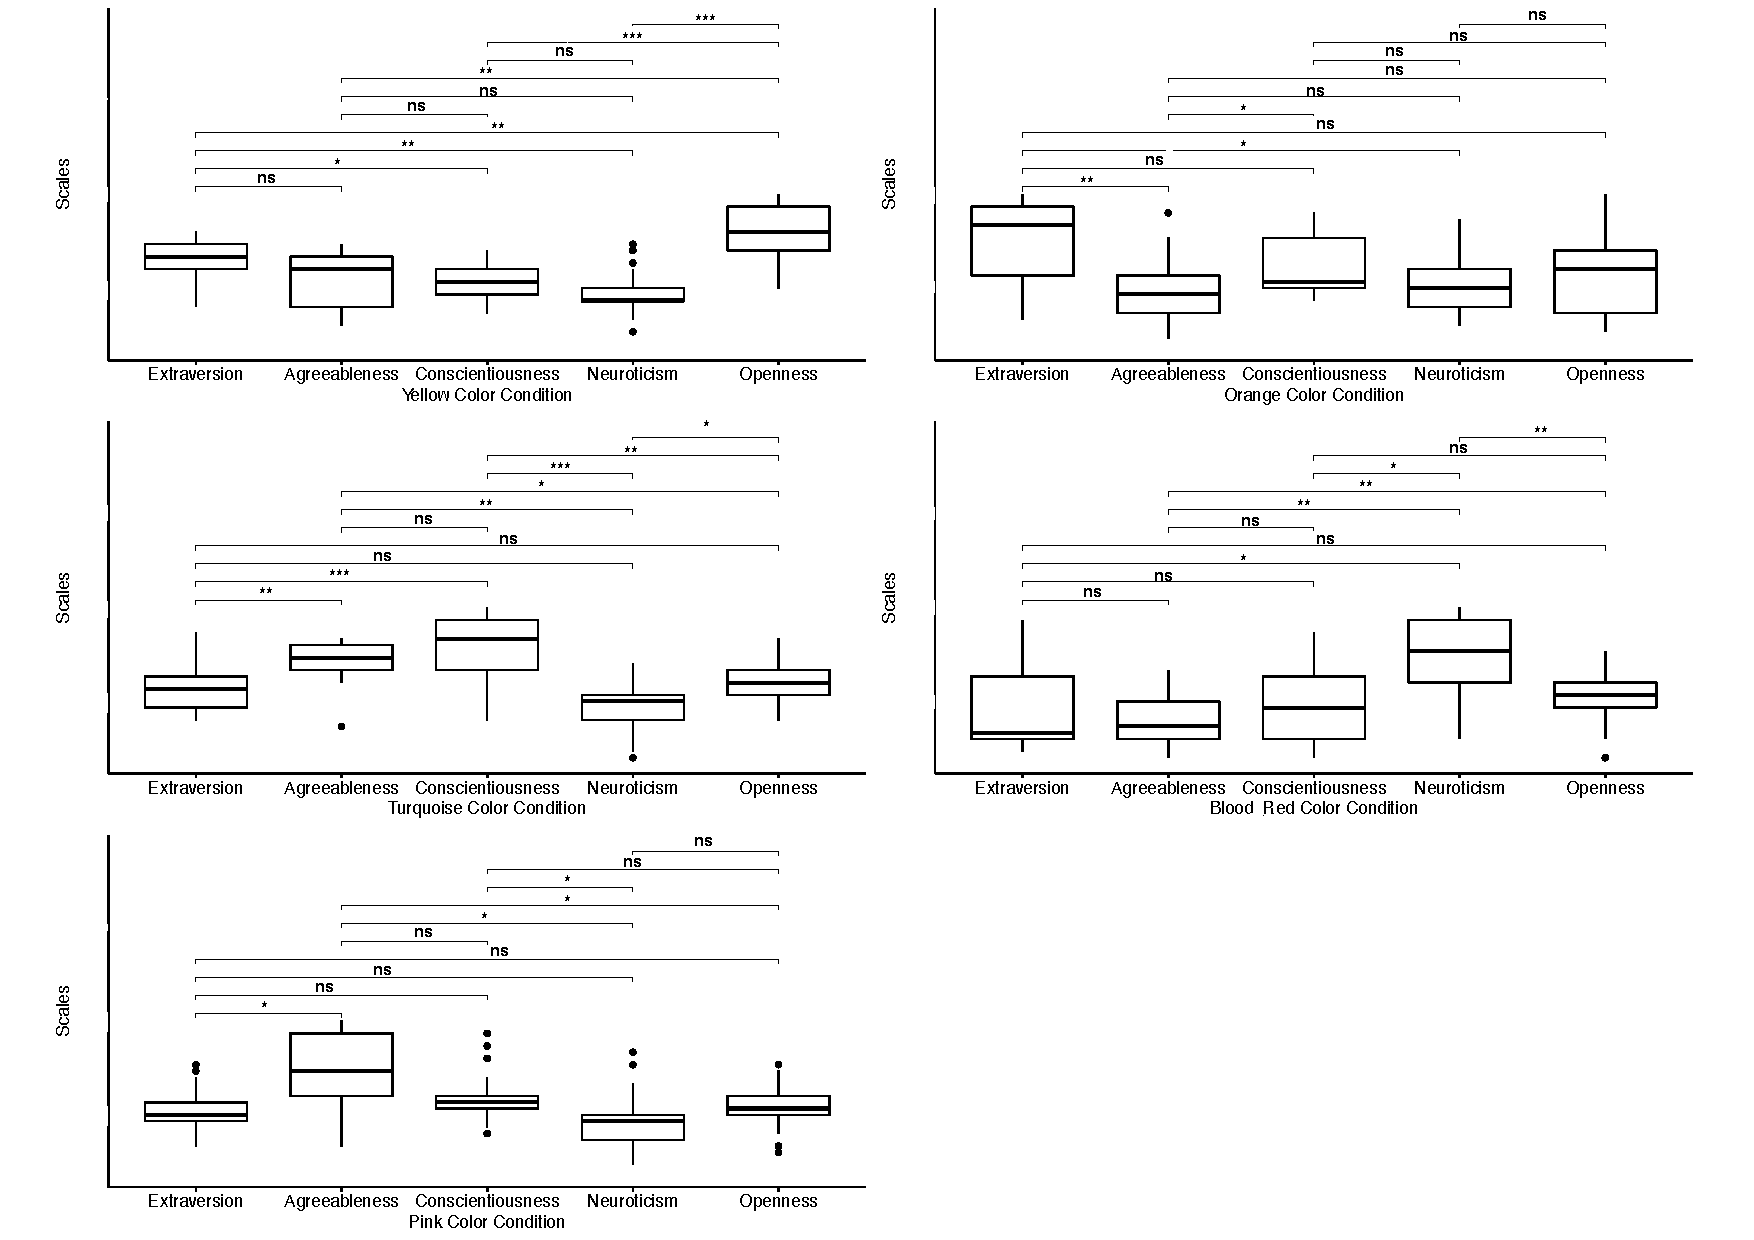
\includegraphics[scale=0.45]{Study2(M-T).pdf}
    \caption{A boxplot for Mascot-Lamp interaction in Study-1}
    \label{fig:MT2}
\end{figure}

% TODO: Table median (values)
% TODO: Figure p-values
% TODO: p-value, df=?

\chapter{Discussions}
\label{ch:discussions}
This chapter covers discussion of the results obtained from the statistical tests.
In this study, the behavior of a mascot is conceptualized four interaction types which are referred as case-studies.
Sections~\ref{sec:mascot-speakers-interaction}, ~\ref{sec:mascot-lamp-interaction},
~\ref{sec:mascot-mascot-interaction}, and ~\ref{sec:mascot-tablet-interaction} discuss each interaction type for the
within personality and the within condition studies.

\section{Mascot-speakers interaction}
\label{sec:mascot-speakers-interaction}
The empirical evidence for mascot-speakers case-study shows that the type of music influences the participants'
interpretation of the personality trait.
The mascot triggering sophisticated, contemporary, or unpretentious song can be associated
with a specific personality trait. \\

\textbf{The discussion of the first study.}\par
On the one hand, the interaction between mascot and contemporary was interpreted
to be more extravert which is characterised as being more friendly,
sociable, cheerful and so on.
On the other hand, this type of interaction also was rated very high on conveying
neuroticism personality trait which is described as being more emotionally unstable,
angry, vulnerable, depressive and so on.
The mascot triggering sophisticated music was perceived to be more open to new experiences.
Such songs as classical, jazz and contemporary adult were interpreted as more artistic intelligent,
thoughtful, and other facets representing openness personality trait (see Table~\ref{table:opennessFacets}).
Agreeableness and conscientiousness personality traits were associated with sophisticated and
unpretentious compared to contemporary music.
However, this study does not provide statistical evidence for these two personality traits to be
conveyed by a specific music type.

\textbf{The discussion of the second study.}\par
The within music condition study revealed that mascot interacting with sophisticated music
was perceived to be more open to new experiences.
In addition, the first study associated contemporary with both extraversion and neuroticism personality traits.
By comparing the ratings of all personality traits within contemporary music, the second study revealed that this
music condition conveys extraversion personality trait most.


\section{Mascot-lamp interaction}
\label{sec:mascot-lamp-interaction}
The study shows that the change in color of the lamp has an impact on the way
how participants interpret the personality of a mascot.
This shows that the lamp that mascot interact with was not only interpreted as an
artificial light source but also gave clues about mascot's personality trait\\

\textbf{The discussion of the first study.}\par
Participants associated mascot triggering blood-red lighting neuroticism personality trait
which is characterized as to be to be highly anxious, angry, depressive, self-conscientious, impulsive and vulnerable.
Extraversion personality was rated very high to be conveyed with yellow lighting only compared
to turquoise, blood-red, and pink.
With agreeableness and conscientiousness, participants rated mascots interacting with pink, yellow,
turquoise lighting to be more associated with these personality traits.
However, for all personality traits except neuroticism, it is hard to distinguish
a specific color that conveys these personality traits.\\

\textbf{The discussion of the second study.}\par
The mascot triggering the blood-red lighting is interpreted to be mor neuroticism as an anxious, highly depressive,
angry, vulnerable, and that has an immoderate behavior.
The second study confirms that how personality of a mascot was measured, except
for neuroticism, all other personality traits cannot be conveyed by a single color.
For example, both turquoise and pink lights convey agreeableness and
conscientiousness personality traits.
Also, orange color was interpreted to be more extravert and openness to new experiences.\\


\section{Mascot-mascot interaction}
\label{sec:mascot-mascot-interaction}
The statistical analysis showed that the levels of vibration have a significant effect on the
measurement of mascot's personality.\\

\textbf{The discussion of the first study.}\par
Participants experiencing 500 milliseconds vibration duration interpreted the approaching mascot as more
energetic, assertive, forceful, energetic, friendly, sociable, cheerful which
constitutes extraversion personality trait.
The mascot interacting with level-2 and level-3 was perceived to be more agreeable which
is described as being modest, cooperative, trustworthy and so on.
Mascot interacting with level-3 and level-4 vibration are interpreted as conscientiousness.
The participants experiencing 100 millisecond vibration aka level-1 interpreted
approaching mascot as neuroticism which is characterized by being
anxious, angry, depressive and so on (see Table~\ref{table:opennessFacets}).\\

\textbf{The discussion of the second study.}\par
Participants experiencing the vibration with the shortest duration
perceived approaching mascot (i.e.\ the mascot that triggered their device) as neurotic.
The mascot causing 200 milliseconds per time interpreted as agreeable.
Th mascot making participant's phone to vibrate with the duration of 500
milliseconds conveys extraversion personality trait.\\

\section{Mascot-tablet interaction}
\label{sec:mascot-tablet-interaction}
The empirical evidences revealed that, overall, the change of background
color effects which personality trait will be perceived by this interaction.\\

\textbf{The discussion of the first study.}\par
For the within personality study, turquoise which is distinguished from all other
colors represents conscientiousness personality trait.
Also, blood-red color is associated with neuroticism personality that is characterized by
having immoderate behavior, being aggressive, depressive and so on.
Openness personality is best conveyed by yellow screen color.\\

\textbf{The discussion of the second study.}\par
The analysis of within each color condition shows that yellow background portrays openness
personality trait which makes the results from the first study even more consistent.
Also, blood-red screen is significantly associated with neuroticism personality.
The first study revealed conscientiousness personality conveyed by turquoise color.
However, when all personality traits were compared within turquoise color, the ratings
of conscientiousness personality trait did not distinguish from the scores given for
agreeableness personality.
Thus, according to the second study turquoise color failed to be associated only with conscientiousness personality.\\

\section{Overview of the discussion}
\label{sec:overview-of-the-discussion}

Associate conditions with the personality traits.
The representation of all types of behavior and associated personality traits.
The results that we obtained from the study is the following:

\begin{itemize}
    \renewcommand{\labelitemi}{$\Rightarrow$}
    \item \textbf{Music type}
    \begin{labeling}{alligator}
        \item [Extraversion:] contemporary songs
        \item [Openness:] sophisticated songs
    \end{labeling}

    \item \textbf{Lighting color}
    \begin{labeling}{alligator}
        \item [Neuroticism:] blood-red
    \end{labeling}

    \item \textbf{Vibration level}
    \begin{labeling}{alligator}
        \item [Neuroticism:] level-1 (100 ms)
        \item [Agreeableness:] level-2 (200 ms)
        \item [Extraversion:] level-5 (500 ms)
    \end{labeling}

    \item \textbf{Screen color}
    \begin{labeling}{alligator}
        \item [Neuroticism:] blood-red
        \item [Openness:] yellow
    \end{labeling}
\end{itemize}
\chapter{Conclusion}
\label{ch:conclusion}
Section 8.1 of the final chapter gives a conclusive overview of the results achieved during conducting this research.
In section 8.2, we describe the contribution and our attempts to improve the system compared to related
work [Chapter 2] and in section 8.3 we provide certain limitations to our study.
Further, in section 8.4, we discuss how the ideas explored in this project can be continued further.

\section{Overview}
\label{sec:overview}
In this study both psychological and user‐experience approaches helps us to better understand thing to thing interaction.

\subsection{The birth of the idea}
\label{subsec:the-birth-of-the-idea}
In our study we started with a question: “What interactive objects with a certain behavior can tell us about itself?”.
Thus, we decided to assign a personality trait to a mascot, assuming that personality
may be identification of this social device.
We hope that the interaction between a mascot and other inanimate devices might be a
descriptive clue for personality of that mascot.
Therefore, the actions that mascot is taking might convey the personality of it.
From analysis point of view, taking into account all possible types of interaction
would cause a huge data set that will be hard to analyze.
Thus, we decided to minimize
possible actions by using Proxemics theory, which helped us to come up with case-studies such
as the interaction between mascot-mascot, mascot-tablet, mascot-lamp, and mascot-speakers.
Further, for each interaction type we had to come up with possible actions such as mascot
triggering specific song or lighting color and so on.
During our study, we have noticed that
certain type of behavior, for example, mascot emitted pink color or
sophisticated song and so on, conveys a particular personality trait.

\subsection{Overview of the results}
\label{subsec:overview-of-the-results}
Now we can review the final results.
We analyzed the data from two perspectives and reported them as study-1 and study-2 in chapter 6.
In the first study, we observe the personality trait and the variation of all
conditions within each personality individually.
In our second study, we take a closer look at each condition and the variation of
all personality traits within a specific condition.
The second study is supplementary for the first study.
When during the first study, we see that one condition conveys several personality traits,
the second study gives us additional information regarding which of these personality
traits conveyed most by this condition.

\par For \textbf{Mascot-lamp interaction}, we can conclude that both studies showed that
there is a positive relationship between blood-red and neuroticism personality.
Thus, if the mascot triggers blood-red lighting as a representation of its behavior,
it will convey the neuroticism personality trait.
Choosing turquoise or pink lighting as a behavior of the
mascot will be measured either as a conscientious or agreeable social device.
The same tendency is observed for orange color, by showing this color, we may convey
either extraversion or openness personality trait.
Unfortunately, for mascot-lamp interaction, yellow lighting failed to portray stable personality trait.

\par For \textbf{Mascot-speakers interaction}, in order to convey extraversion or neuroticism personality traits,
contemporary music will be the best choice.
For the mascot that attributes an openness personality trait,
the good choice will fall on sophisticated music.
Or the other way around, by choosing sophisticated music, the personality trait that
will be conveyed is an openness.
When we choose contemporary music, the mascot will convey an extraversion personality trait.
In our first study, we notice that both extraversion and neuroticism are positively related to contemporary music.
Having two personalities related to the same music category, our second study
revealed that when choosing contemporary music, extraversion personality will be conveyed more.

\par For \textbf{Mascot-mascot interaction}, extraversion mascot can be presented by
showing higher levels of vibration, namely Level-4 and Level-5.
If we assign agreeableness personality to our mascot or any other social device,
the good choice will be focusing on Level-2 and Level-3.
For conscientious mascot, we can take Level-3 and Level-4 as a representational behavior of that personality trait.
When we want to convey the neuroticism personality trait, we make a choice for Level-1,
the vibration with the lowest duration.
And vice versa, as a result of the second study, Level-1 will convey that the mascot
is neurotic, Level-2 - agreeable, and Level-5 that the mascot is an extravert.
Moreover, by choosing Level-3, we will able to portray either agreeableness or conscientious personality traits.
And by choosing Level-4, both extraversion and conscientiousness personalities can be conveyed.

\par For \textbf{Mascot-tablet interaction}, in order to convey the conscientiousness personality trait,
mascot should be able to trigger a tablet to display turquoise color.
Whereas, for a neurotic mascot, the blood-red may be a good and distinctive choice.
Finally, when we want to convey an openness personality trait, the mascot should represent yellow color.
Further, if we want to focus on colors, yellow screen color is a good choice to convey openness,
blood-red portrays neuroticism personality trait.
In addition, turquoise and pink screen colors can exhibit either agreeableness or
conscientious personality traits.
The last two colors may need further study.

\par Despite the fact that yellow lighting could not convey any personality traits for
mascot-lamp interaction, there is a clear positive relationship between yellow screen color
and mascot’s openness personality trait for mascot-tablet interaction.
We can assume that the reason for a different interpretation of the same color in different
case-studies is that the lamp emitting yellow light can be perceived as the
typical color you get from incandescent bulbs.
Meanwhile, the yellow screen color is perceived as a more vivid color framed in a screen.
The same observation is made for blood-red color which conveys a neurotic personality trait for both case-studies.
However, the mascot triggering the lamp with blood-red lighting is perceived as
more angry, anxious, depressive, emotionally unstable and impulsive than the
mascot triggering the same color in the tablet.
We can assume that by illuminating the whole room with blood-red color people can
get a more negative impression about mascot’s personality than seeing the same color in a tablet-size screen.

\section{Contributions and findings}
\label{sec:contributions-and-findings}
The main contribution is an achieving cooperation among mascot and other interactive
objects in a system where each mascot has a unique personality trait.
This can, in turn, serve as a contribution for designing social devices in SIoT environment.
Moreover, the networthing finding is that there is a relationship between
personality trait and behavior of interactive objects.
Although this relationship is not as clear and vivid as we observe in human-human interaction,
it is a good insight that personality and behavior are interconnected concepts even for inanimate objects.
These concepts can help engineers to design their social devices and to serve as an
aid for users to better understand interaction between them.
For example, when researchers or engineers would like to construct SIoT devices
with certain personalities they could use our findings about types of behavior that can
convey this personality trait.
We hope that behavior that we came up with, particularly four types of interaction shed
a light on how behavior of social devices can help people to understand their personality and
therefore, the main goals, intentions, and motivation of inanimate object.
When engineers try to configure personality on social device in the context of behaviour and
interaction types that we described they can expect actions that we reported in chapter 6.
On the other hand if researchers or engineers set up specific commands i.e actions to the
social device the users will understand the device's personality as we described in discussion chapter.

\par Moreover, there is one unexpected phenomenon that we observed during experiments.
We know that each participant has its own approach on measuring the personality traits of a mascot.
So, before experiment, we believed that while measuring the mascot’s personality,
participants will rely on their background knowledge of non-verbal clues such as favorite colors or music and so on.
However, during the experiments, we noticed that some participants did not focus on
factors such as lighting, music and etc as pure independent variable that is affecting their choice.
During post-experiment discussions, we noticed that they first associated these factors with
someone from their life and then analyze the mascot as they would assess that person.
This was an interesting finding showing that some people would prefer to measure the
personality of social device by relating it to the real world scenarios and making
references to the person from real-world.
Of course, this observation is hard to extend to a whole population.
However, it was an easter egg in a sense that when people were observing the
interaction between social devices, they immediately applied anthropomorphic rules
even if they knew that these are inanimate objects.

\section{Limitations}
\label{sec:limitations}
Unfortunately, the study was based on relatively small (N=25) and homogeneous
(e.g. having 70\% of participants from formal sciences and age mean of 26) samples which
limited the power of their analyses and make it difficult to extrapolate findings to a general population.
However, the experiment design was counterbalanced in terms of other important
characteristics such as gender, participants’ overall music preferences for mascot-speakers
interaction and the order in which participants watched the videos.

\par Another limitation could be that the study was held in a laboratory setting where
participants only had a limited time to assess the personalities of mascots.
On the one hand, there is a possibility that spending more time (i.e. hours or days)
with mascots could affect participant’s opinions on assigning the personality trait to these devices.
On the other hand, during these experiments participants reflected their very first impressions
while seeing the interaction between devices and their initial reaction while measuring the
personality traits of mascot based on these interactions.

\par The results did not reveal full pattern where we can state that certain personality
can be conveyed with the following color, vibration level and music genre.
However, we shed a light on the impact of these factors can have an perceiving the personality of social device.
Despite the fact that some of the factors were hard to measure as a behavior of certain personalities,
Table(conclusion) gave us an insight that personality of social devices and their behavior
are interconnected concepts.
Moreover, some of these personality traits can be ??vividly conveyed by pre-defined factors.


\section{Future work}
\label{sec:future-work}
\par In future work, design researchers interested in contributing to our study can focus
on finer specifications of factors.
These specifications can be either toward new interaction types and behavior or toward
improvement of the results from existing interactions.
Testing more songs from different genres, or more colors for light and screen may serve as a good example.
Another idea might be improving mascot-tablet interaction in addition to screen colors
some other functionalities can be added.
For example, when mascot approaching tablet it can show some favorite pictures in order
to give more information about mascot.
In fact, the design of such system should also take into account security aspects for not leaking personal photos.

\par Another approach might be using the interaction between social devices as a trigger or
motivation for people to socialize and communicate more.
The behavior of mascots such as trigger lighting or music play or vibrate some other
person’s mascot when you approach it, can be an icebreaker for people to communicate with each other.

\appendix
%\chapter{Tables and Figures}
%
%\begin{longtable} { |p{0.5cm}| p{2cm}|p{2cm}|p{1.5cm}| p{1.7cm}|p{1cm}|p{1.5cm}|  }
%    \captionsetup{width=13.5cm}
%    \caption{The statistically significant comparisons of each group individually using the Wilcoxon signed-rank test
%    and Bonferroni correction while measuring Five Personality Traits for Mascot-Lamp interaction. In addition reporting
%    effect sizes which are large}
%    \label{table:wilcoxML1} \\
%    \hline
%    \multicolumn{1}{| c}{}
%    &\multicolumn{1}{| c}{\textbf{Group 1}}
%    & \multicolumn{1}{| c}{\textbf{Group 2}}
%    & \multicolumn{2}{| c |}{\textbf{Wilcoxon tests}}
%    & \multicolumn{1}{c}{\textbf{r}}
%    & \multicolumn{1}{| c |}{\textbf{padj}} \\
%    & 	&	  & \textbf{z} & \textbf{p} & &	     \\
%    \hline
%    \endfirsthead
%    \multicolumn{7}{c}%
%    {\tablename\ \thetable\ -- \textit{Continued from previous page}} \\
%    \hline
%    \multicolumn{1}{| c}{}
%    &\multicolumn{1}{| c}{\textbf{Group 1}}
%    & \multicolumn{1}{| c}{\textbf{Group 2}}
%    & \multicolumn{2}{| c |}{\textbf{Wilcoxon tests}}
%    & \multicolumn{1}{c}{\textbf{r}}
%    & \multicolumn{1}{| c |}{\textbf{padj}} \\
%    & 	&	  & \textbf{z} & \textbf{p} & &	     \\
%    \hline
%    \endhead
%    \hline \multicolumn{7}{r}{\textit{Continued on next page}} \\
%    \endfoot
%    \hline
%    \endlastfoot
%    \multirow{6}{*}{\textbf{E}}
%    &Yellow		&Turquoise	&3.5315	&p<0.01	&0.706	&p<0.01\\
%    &Yellow		&Blood-Red	&4.185	&p<0.01	&0.837	&p<0.01\\
%    &Yellow		&Pink		&3.8951	&p<0.01	&0.781	&p<0.01\\
%    &Orange		&Blood-Red	&4.1461	&p<0.01	&0.829	&p<0.01\\
%    &Turquoise	&Blood-Red	&3.3966	&p<0.01	&0.682	&p<0.01\\
%    &Blood-Red	&Pink		&-3.5166	&p<0.01	&0.711	&p<0.01\\
%    \hline
%    \hline
%    \multirow{6}{*}{\textbf{A}}
%    &Yellow		&Orange		&3.6211	&p<0.01	&0.724		&p<0.01\\
%    &Yellow		&Blood-Red	&4.0237	&p<0.01	&0.805		&p<0.01\\
%    &Orange		&Turquoise	&-4.0613	&p<0.01	&0.832		&p<0.01\\
%    &Orange		&Pink		&-4.294	&p<0.01	&0.859		&p<0.01\\
%    &Turquoise	&Blood-Red	&4.2807	&p<0.01	&0.856		&p<0.01\\
%    &Blood-Red	&Pink		&-4.1868	&p<0.01	&0.842		&p<0.01\\
%    \hline
%    \hline
%    \multirow{6}{*}{\textbf{C}}
%    &Yellow		&Orange		&3.3333	&p<0.01	&0.660		&p<0.01\\
%    &Yellow		&Blood-Red	&3.1945	&p<0.01	&0.657 		&p<0.05\\
%    &Orange		&Turquoise	&-3.8186	&p<0.01	&0.767		&p<0.01\\
%    &Orange		&Pink		&-3.7784	&p<0.01	&0.755		&p<0.01\\
%    &Turquoise	&Blood-Red	&3.2405	&p<0.01	&0.644		&p<0.05\\
%    &Blood-Red	&Pink		&-3.1456	&p<0.01	&0.619		&p<0.05\\
%    \hline
%    \hline
%    \multirow{4}{*}{\textbf{N}}
%    &Yellow		&Blood-Red	&-4.3193	&p<0.01	&0.864		&p<0.01\\
%    &Orange		&Blood-Red	&-4.2602	&p<0.01	&0.862		&p<0.01\\
%    &Turquoise	&Blood-Red	&-4.287	&p<0.01	&0.872		&p<0.01\\
%    &Blood-Red	&Pink		&4.3738	&p<0.01	&0.875		&p<0.01\\
%    \hline
%    \hline
%    \multirow{4}{*}{\textbf{O}}
%    &Yellow		&Blood-Red	&3.4619	&p<0.01	&0.692		&p<0.01\\
%    &Yellow		&Pink		&2.8482	&p<0.01	&0.574		&p<0.05\\
%    &Orange		&Blood-Red	&3.0702	&p<0.01	&0.614		&p<0.05\\
%    \hline
%\end{longtable}
%
%\begin{longtable}{ |p{1.9cm}| p{0.5cm}|p{0.5cm}|p{1.2cm}| p{1.9cm}|p{1cm}|p{1.5cm}|  }
%    \captionsetup{width=13.5cm}
%    \caption{Mascot-Lamp interaction}
%    \label{table:wilcoxML2} \\
%    \hline
%    \multicolumn{1}{| c}{}
%    &\multicolumn{1}{| c}{\textbf{Group 1}}
%    & \multicolumn{1}{| c}{\textbf{Group 2}}
%    & \multicolumn{2}{| c |}{\textbf{Wilcoxon tests}}
%    & \multicolumn{1}{c}{\textbf{r}}
%    & \multicolumn{1}{| c |}{\textbf{padj}} \\
%    & 	&	  & \textbf{z} & \textbf{p} & &	     \\
%    \hline
%    \endfirsthead
%    \multicolumn{7}{c}%
%    {\tablename\ \thetable\ -- \textit{Continued from previous page}} \\
%    \hline
%    \multicolumn{1}{| c}{}
%    &\multicolumn{1}{| c}{\textbf{Group 1}}
%    & \multicolumn{1}{| c}{\textbf{Group 2}}
%    & \multicolumn{2}{| c |}{\textbf{Wilcoxon tests}}
%    & \multicolumn{1}{c}{\textbf{r}}
%    & \multicolumn{1}{| c |}{\textbf{padj}} \\
%    & 	&	  & \textbf{z} & \textbf{p} & &	     \\
%    \hline
%    \endhead
%    \hline \multicolumn{7}{r}{\textit{Continued on next page}} \\
%    \endfoot
%    \hline
%    \endlastfoot
%    \multirow{4}{*}{\textbf{Yellow}}
%    &E	&N	&3.9296		&p<0.01	&0.789	&p<0.01\\
%    &A	&N	&3.561		&p<0.01	&0.722	&p<0.01\\
%    &C	&N	&3.4599		&p<0.01	&0.692	&p<0.01\\
%    &N	&O	&-3.6295		&p<0.01	&0.721	&p<0.01\\
%    \hline
%    \hline
%    \multirow{6}{*}{\textbf{Orange}}
%    &E	&A	&4.0294		&p<0.01	&0.818	&p<0.01\\
%    &E	&C	&0.679		&p<0.01	&0.679	&p<0.01\\
%    &E	&N	&0.661		&p<0.01	&0.661	&p<0.01\\
%    &A	&O	&-4.1086		&p<0.01	&0.840	&p<0.01\\
%    &C	&O	&-2.9182		&p<0.01	&0.587	&p<0.05\\
%    &N	&O	&-3.1376		&p<0.01	&0.636	&p<0.05\\
%    \hline
%    \hline
%    \multirow{8}{*}{\textbf{Turquoise}}
%    &E			&A				&-3.8621			&p<0.01			&0.776		&p<0.01\\
%    &E			&C				&-3.339			&p<0.01			&0.668		&p<0.01\\
%    &E			&N				&3.0291			&p<0.01			&0.617		&p<0.05\\
%    &A			&N				&3.7697			&p<0.01			&0.754		&p<0.01\\
%    &A			&O				&2.8456			&p<0.01			&0.552		&p<0.05\\
%    &C			&N				&4.1879			&p<0.01			&0.843		&p<0.01\\
%    &C			&O				&3.4339			&p<0.01			&0.687		&p<0.01\\
%    &N			&O				&-3.4777			&p<0.01			&0.690 		&p<0.01\\
%    \hline
%    \hline
%    \multirow{7}{*}{\textbf{Blood Red}}
%    &E			&N				&-4.3464			&p<0.01			&0.869		&p<0.01\\
%    &E			&O				&-2.9088			&p<0.01			&0.596		&p<0.05\\
%    &A			&C				&-2.9421			&p<0.01			&0.597		&p<0.05\\
%    &A			&N				&-4.2335			&p<0.01			&0.857		&p<0.01\\
%    &A			&O				&-3.2177			&p<0.01			&0.631		&p<0.05\\
%    &C			&N				&-3.8625			&p<0.01			&0.773		&p<0.01\\
%    &N			&O				&3.9709			&p<0.01			&0.794		&p<0.01\\
%    \hline
%    \hline
%    \multirow{8}{*}{\textbf{Pink}}
%    &E			&A				&-3.9842			&p<0.01			&0.797		&p<0.01\\
%    &E			&C				&-3.4545			&p<0.01			&0.714		&p<0.01\\
%    &E			&N				&3.6722			&p<0.01			&0.735		&p<0.01\\
%    &A			&N				&4.2394			&p<0.01			&0.848		&p<0.01\\
%    &A			&O				&3.9193			&p<0.01			&0.792		&p<0.01\\
%    &C			&N				&4.2392			&p<0.01			&0.848		&p<0.01\\
%    &C			&O				&3.1883			&p<0.01			&0.638		&p<0.05\\
%    &N			&O				&-3.9322			&p<0.01			&0.794		&p<0.01\\
%    \hline
%\end{longtable}
%
%\begin{longtable}{ |p{0.3cm}| p{2.4cm}|p{2.4cm}|p{1.2cm}| p{1.7cm}|p{1cm}|p{1.7cm}|  }
%    \captionsetup{width=13.5cm}
%    \caption{The statistically significant comparisons of each group individually using the Wilcoxon signed-rank test and
%    Bonferroni correction while measuring Five Personality Traits for Mascot-Speakers interaction. In addition reporting
%    effect sizes which are large}
%    \label{table:wilcoxMS1} \\
%    \hline
%    \multicolumn{1}{| c}{}
%    &\multicolumn{1}{| c}{\textbf{Group 1}}
%    & \multicolumn{1}{| c}{\textbf{Group 2}}
%    & \multicolumn{2}{| c |}{\textbf{Wilcoxon tests}}
%    & \multicolumn{1}{c}{\textbf{r}}
%    & \multicolumn{1}{| c |}{\textbf{padj}} \\
%    & 	&	  & \textbf{z} & \textbf{p} & &	     \\
%    \hline
%    \endfirsthead
%    \multicolumn{7}{c}%
%    {\tablename\ \thetable\ -- \textit{Continued from previous page}} \\
%    \hline
%    \multicolumn{1}{| c}{}
%    &\multicolumn{1}{| c}{\textbf{Group 1}}
%    & \multicolumn{1}{| c}{\textbf{Group 2}}
%    & \multicolumn{2}{| c |}{\textbf{Wilcoxon tests}}
%    & \multicolumn{1}{c}{\textbf{r}}
%    & \multicolumn{1}{| c |}{\textbf{padj}} \\
%    & 	&	  & \textbf{z} & \textbf{p} & &	     \\
%    \hline
%    \endhead
%    \hline \multicolumn{7}{r}{\textit{Continued on next page}} \\
%    \endfoot
%    \hline
%    \endlastfoot
%    \multirow{3}{*}{\textbf{E}}
%    &Sophisticated		&Contemporary			&-4.2111			&p<0.01		&0.842 		&p<0.01\\
%    &Sophisticated		&Unpretentious			&-2.7188			&p<0.01		&0.544 		&p<0.05\\
%    &Contemporary		&Unpretentious			&3.8751			&p<0.01		&0.775		&p<0.01\\
%    \hline
%    \hline
%    \multirow{2}{*}{\textbf{A}}
%    &Sophisticated		&Contemporary			&4.2864			&p<0.01		&0.872 	&p<0.01\\
%    &Contemporary		&Unpretentious			&-4.2121			&p<0.01		&0.842 	&p<0.01\\
%    \hline
%    \hline
%    \multirow{2}{*}{\textbf{C}}
%    &Sophisticated		&Contemporary			&3.0545			&p<0.01		&0.611 		&p<0.01\\
%    &Contemporary		&Unpretentious			&-2.7863			& p<0.01		& 0.546 		&p<0.05\\
%    \hline
%    \hline
%    \multirow{2}{*}{\textbf{N}}
%    &Sophisticated		&Contemporary			&-3.9739			&p<0.01		& 0.797		&p<0.01\\
%    &Contemporary		&Unpretentious			&3.7269			&p<0.01		&0.745 		&p<0.01\\
%    \hline
%    \hline
%    \multirow{3}{*}{\textbf{O}}
%    &Sophisticated		&Contemporary			&4.2932			&p<0.01		& 0.859 		&p<0.01\\
%    &Sophisticated		&Unpretentious			&2.9869			&p<0.01		& 0.595 		&p<0.01\\
%    &Contemporary		&Unpretentious			&-3.9709			&p<0.01		& 0.794  		&p<0.01\\
%    \hline
%\end{longtable}
%
%\begin{longtable}{ |p{2.5cm}| p{0.5cm}|p{0.5cm}|p{1.3cm}| p{1.7cm}|p{1cm}|p{1.7cm}|  }
%    \captionsetup{width=13.5cm}
%    \caption{Mascot-Speakers}
%    \label{table:wilcoxMS2} \\
%    \hline
%    \multicolumn{1}{| c}{}
%    &\multicolumn{1}{| c}{\textbf{Group 1}}
%    & \multicolumn{1}{| c}{\textbf{Group 2}}
%    & \multicolumn{2}{| c |}{\textbf{Wilcoxon tests}}
%    & \multicolumn{1}{c}{\textbf{r}}
%    & \multicolumn{1}{| c |}{\textbf{padj}} \\
%    & 	&	  & \textbf{z} & \textbf{p} & &	     \\
%    \hline
%    \endfirsthead
%    \multicolumn{7}{c}%
%    {\tablename\ \thetable\ -- \textit{Continued from previous page}} \\
%    \hline
%    \multicolumn{1}{| c}{}
%    &\multicolumn{1}{| c}{\textbf{Group 1}}
%    & \multicolumn{1}{| c}{\textbf{Group 2}}
%    & \multicolumn{2}{| c |}{\textbf{Wilcoxon tests}}
%    & \multicolumn{1}{c}{\textbf{r}}
%    & \multicolumn{1}{| c |}{\textbf{padj}} \\
%    & 	&	  & \textbf{z} & \textbf{p} & &	     \\
%    \hline
%    \endhead
%    \hline \multicolumn{7}{r}{\textit{Continued on next page}} \\
%    \endfoot
%    \hline
%    \endlastfoot
%    \multirow{9}{*}{\textbf{Sophisticated}}
%    &E		&A			&-3.9431			&p<0.01			&0.789 		&p<0.01\\
%    &E		&N			&3.6469			&p<0.01			&0.729 		&p<0.01\\
%    &E		&O			&-4.3459			&p<0.01			&0.869		&p<0.01\\
%    &A		&C			&2.8937			& p<0.01			&0.579 		&p<0.05\\
%    &A		&N			&4.3732			&p<0.01			&0.875 		&p<0.01\\
%    &A		&O			&-3.3377			&p<0.01			&0.668 		&p<0.01\\
%    &C		&N			&4.1446			&p<0.01			&0.829 		&p<0.01\\
%    &C		&O			&-3.8436			&p<0.01			&0.762 		&p<0.01\\
%    &N		&O			&-4.373			&p<0.01			&0.875 		&p<0.01\\
%    \hline
%    \hline
%    \multirow{4}{*}{\textbf{Contemporary}}
%    &E		&A			&4.2574			&p<0.01			&0.861 		&p<0.01\\
%    &E		&C			&4.2659			&p<0.01			&0.853		&p<0.01\\
%    &E		&N			&4.1175			&p<0.01			&0.824 		&p<0.01\\
%    &E		&O			&4.2866			&p<0.01			&0.872 		&p<0.01\\
%    \hline
%    \hline
%    \multirow{7}{*}{\textbf{Unpretentious}}
%    &E		&A			&-3.1034			&p<0.01			& 0.630  		&p<0.05\\
%    &E		&N			&4.3736			&p<0.01			& 0.875		&p<0.01\\
%    &A		&C			&3.4615			&p<0.01			& 0.742		&p<0.01\\
%    &A		&N			&4.3463			&p<0.01			& 0.869 		&p<0.01\\
%    &C		&N			&3.7949			&p<0.01			& 0.759		&p<0.01\\
%    &C		&O			&-2.9387			&p<0.01			& 0.569 		&p<0.05\\
%    &N		&O			&-4.3734			&p<0.01			& 0.875		&p<0.01\\
%    \hline
%\end{longtable}
%
%\begin{longtable}{ |p{0.5cm}| p{1.5cm}|p{1.5cm}|p{1.3cm}| p{1.6cm}|p{1cm}|p{1.5cm}|  }
%    \captionsetup{width=13.5cm}
%    \caption{The statistically significant comparisons of each group individually using the Wilcoxon signed-rank test and
%    Bonferroni correction while measuring Five Personality Traits for Mascot-Mascot interaction. In addition reporting
%    effect sizes which are large}
%    \label{table:wilcoxMM1} \\
%    \hline
%    \multicolumn{1}{| c}{}
%    &\multicolumn{1}{| c}{\textbf{Group 1}}
%    & \multicolumn{1}{| c}{\textbf{Group 2}}
%    & \multicolumn{2}{| c |}{\textbf{Wilcoxon tests}}
%    & \multicolumn{1}{c}{\textbf{r}}
%    & \multicolumn{1}{| c |}{\textbf{padj}} \\
%    & 	&	  & \textbf{z} & \textbf{p} & &	     \\
%    \hline
%    \endfirsthead
%    \multicolumn{7}{c}%
%    {\tablename\ \thetable\ -- \textit{Continued from previous page}} \\
%    \hline
%    \multicolumn{1}{| c}{}
%    &\multicolumn{1}{| c}{\textbf{Group 1}}
%    & \multicolumn{1}{| c}{\textbf{Group 2}}
%    & \multicolumn{2}{| c |}{\textbf{Wilcoxon tests}}
%    & \multicolumn{1}{c}{\textbf{r}}
%    & \multicolumn{1}{| c |}{\textbf{padj}} \\
%    & 	&	  & \textbf{z} & \textbf{p} & &	     \\
%    \hline
%    \endhead
%    \hline \multicolumn{7}{r}{\textit{Continued on next page}} \\
%    \endfoot
%    \hline
%    \endlastfoot
%    \multirow{6}{*}{\textbf{E}}
%    &Level-1		&Level-4			&-3.9316			&p<0.01			& 0.786		&p<0.01\\
%    &Level-1		&Level-5			&-3.5756			&p<0.01			& 0.714		&p<0.01\\
%    &Level-2		&Level-4			&-3.687			&p<0.01			&0.743 		&p<0.01\\
%    &Level-2		&Level-5			&-3.4301			&p<0.01			&0.678 		&p<0.01\\
%    &Level-3		&Level-4			&-3.545			&p<0.01			&0.708 		&p<0.01\\
%    &Level-3		&Level-5			&-2.9168			&p<0.01			& 0.582 		&p<0.05\\
%    \hline
%    \hline
%    \multirow{6}{*}{\textbf{A}}
%    &Level-1		&Level-2			&-3.5566			&p<0.01			&0.703 		&p<0.01\\
%    &Level-1		&Level-3			&-3.6336			&p<0.01			&0.727		&p<0.01\\
%    &Level-2		&Level-4			&3.028			&p<0.01			&0.595 		&p<0.05\\
%    &Level-2		&Level-5			&3.0421			&p<0.01			&0.608 		&p<0.05\\
%    &Level-3		&Level-4			&3.0827			&p<0.01			&0.617 		&p<0.05\\
%    &Level-3		&Level-5			&2.8476			&p<0.01			&0.552		&p<0.05\\
%    \hline
%    \hline
%    \multirow{6}{*}{\textbf{C}}
%    &Level-1		&Level-3			&-3.8995			&p<0.01			&0.809 		&p<0.01\\
%    &Level-1		&Level-4			&-4.0659			&p<0.01			&0.813 		&p<0.01\\
%    &Level-2		&Level-3			&-3.3019			&p<0.01			&0.657		&p<0.01\\
%    &Level-2		&Level-4			&-3.817			&p<0.01			&0.767 		&p<0.01\\
%    &Level-3		&Level-5			&3.3624			&p<0.01			&0.671 		&p<0.01\\
%    &Level-4		&Level-5			&3.8499			&p<0.01			&0.784 		&p<0.01\\
%    \hline
%    \hline
%    \multirow{4}{*}{\textbf{N}}
%    &Level-1		&Level-2			&3.326			&p<0.01			&0.665 		&p<0.01\\
%    &Level-1		&Level-3			&3.8172			&p<0.01			&0.779 		&p<0.01\\
%    &Level-1		&Level-4			&3.8607			&p<0.01			&0.776  		&p<0.01\\
%    &Level-1		&Level-5			&3.4724			&p<0.01			&0.694		&p<0.05\\
%    \hline
%    \hline
%    \multirow{1}{*}{\textbf{O}}
%    &Level-1		&Level-2			&-2.8243			&p<0.01			&0.578 		&p<0.01\\
%    \hline
%\end{longtable}
%
%\begin{longtable}{ |p{1.3cm}| p{0.5cm}|p{0.5cm}|p{1.2cm}| p{1.7cm}|p{1cm}|p{1.5cm}|  }
%    \captionsetup{width=13.5cm}
%    \caption{Mascot-Mascot}
%    \label{table:wilcoxMM2} \\
%    \hline
%    \multicolumn{1}{| c}{}
%    &\multicolumn{1}{| c}{\textbf{Group 1}}
%    & \multicolumn{1}{| c}{\textbf{Group 2}}
%    & \multicolumn{2}{| c |}{\textbf{Wilcoxon tests}}
%    & \multicolumn{1}{c}{\textbf{r}}
%    & \multicolumn{1}{| c |}{\textbf{padj}} \\
%    & 	&	  & \textbf{z} & \textbf{p} & &	     \\
%    \hline
%    \endfirsthead
%    \multicolumn{7}{c}%
%    {\tablename\ \thetable\ -- \textit{Continued from previous page}} \\
%    \hline
%    \multicolumn{1}{| c}{}
%    &\multicolumn{1}{| c}{\textbf{Group 1}}
%    & \multicolumn{1}{| c}{\textbf{Group 2}}
%    & \multicolumn{2}{| c |}{\textbf{Wilcoxon tests}}
%    & \multicolumn{1}{c}{\textbf{r}}
%    & \multicolumn{1}{| c |}{\textbf{padj}} \\
%    & 	&	  & \textbf{z} & \textbf{p} & &	     \\
%    \hline
%    \endhead
%    \hline \multicolumn{7}{r}{\textit{Continued on next page}} \\
%    \endfoot
%    \hline
%    \endlastfoot
%    \multirow{5}{*}{\textbf{Level-1}}
%    &E		&A			&-2.9843			&p<0.01			&0.609 		&p<0.05\\
%    &E		&N			&-3.3934			&p<0.01			&0.671 		&p<0.01\\
%    &A		&N			&-3.0749			&p<0.01			&0.603 		&p<0.05\\
%    &C		&N			&-3.0975			&p<0.01			&0.620 		&p<0.05\\
%    &N		&O			&3.0542			&p<0.01			&0.604 		&p<0.05\\
%    \hline
%    \hline
%    \multirow{4}{*}{\textbf{Level-2}}
%    &E		&A			&-3.7586			&p<0.01			&0.757 		&p<0.01\\
%    &A		&C			&3.1519			&p<0.01			&0.620 		&p<0.05\\
%    &A		&N			&3.3024			&p<0.01			&0.654 		&p<0.01\\
%    &A		&O			&3.1503			&p<0.01			&0.617 		&p<0.05\\
%    \hline
%    \hline
%    \multirow{7}{*}{\textbf{Level-3}}
%    &E		&A			&-2.9298			&p<0.01			&0.584 		&p<0.05\\
%    &E		&C			&-3.3928			&p<0.01			&0.660 		&p<0.01\\
%    &A		&N			&3.8758			&p<0.01			&0.775 		&p<0.01\\
%    &A		&O			&3.303			&p<0.01			& 0.660		&p<0.01\\
%    &C		&N			&4.039			&p<0.01			& 0.808		&p<0.01\\
%    &C		&O			&3.6229			&p<0.01			& 0.722		&p<0.01\\
%    &N		&O			&-3.1867			&p<0.01			&0.627 		&p<0.05\\
%    \hline
%    \hline
%    \multirow{6}{*}{\textbf{Level-4}}
%    &E		&A			&3.5903			&p<0.01			&0.719 		&p<0.01\\
%    &E		&N			&4.1601			&p<0.01			&0.837 		&p<0.01\\
%    &E		&O			&3.8034			&p<0.01			&0.765		&p<0.01\\
%    &A		&C			&-3.7747			&p<0.01			&0.759 		&p<0.01\\
%    &C		&N			&4.1315			&p<0.01			&0.826 		&p<0.01\\
%    &C		&O			&3.7164			&p<0.01			&0.738 		&p<0.01\\
%    \hline
%    \hline
%    \multirow{4}{*}{\textbf{Level-5}}
%    &E		&A			&2.9346			&p<0.01			&0.587 		&p<0.05\\
%    &E		&C			&3.1512			&p<0.01			&0.617 		&p<0.05\\
%    &E		&N			&3.7113			&p<0.01			&0.748 		&p<0.01\\
%    &E		&O			&3.4195			&p<0.01			&0.684 		&p<0.01\\
%    \hline
%\end{longtable}
%
%\begin{longtable}{ |p{0.5cm}| p{1.9cm}|p{1.9cm}|p{1.2cm}| p{1.7cm}|p{1cm}|p{1.5cm}|  }
%    \captionsetup{width=13.5cm}
%    \caption{The statistically significant comparisons of each group individually using the Wilcoxon signed-rank test
%    and Bonferroni correction while measuring Five Personality Traits for Mascot-Tablet interaction. In addition reporting
%    effect sizes which are large }
%    \label{table:wilcoxMT1} \\
%    \hline
%    \multicolumn{1}{| c}{}
%    &\multicolumn{1}{| c}{\textbf{Group 1}}
%    & \multicolumn{1}{| c}{\textbf{Group 2}}
%    & \multicolumn{2}{| c |}{\textbf{Wilcoxon tests}}
%    & \multicolumn{1}{c}{\textbf{r}}
%    & \multicolumn{1}{| c |}{\textbf{padj}} \\
%    & 	&	  & \textbf{z} & \textbf{p} & &	     \\
%    \hline
%    \endfirsthead
%    \multicolumn{7}{c}%
%    {\tablename\ \thetable\ -- \textit{Continued from previous page}} \\
%    \hline
%    \multicolumn{1}{| c}{}
%    &\multicolumn{1}{| c}{\textbf{Group 1}}
%    & \multicolumn{1}{| c}{\textbf{Group 2}}
%    & \multicolumn{2}{| c |}{\textbf{Wilcoxon tests}}
%    & \multicolumn{1}{c}{\textbf{r}}
%    & \multicolumn{1}{| c |}{\textbf{padj}} \\
%    & 	&	  & \textbf{z} & \textbf{p} & &	     \\
%    \hline
%    \endhead
%    \hline \multicolumn{7}{r}{\textit{Continued on next page}} \\
%    \endfoot
%    \hline
%    \endlastfoot
%    \multirow{4}{*}{\textbf{E}}
%    &Yellow		&Blood-Red			&3.1011			&p<0.01			& 0.627 		&p<0.05\\
%    &Yellow		&Pink				&3.2335			&p<0.01			&0.650 		&p<0.05\\
%    &Orange		&Blood-Red			&3.7314			&p<0.01			& 0.751		&p<0.01\\
%    &Orange		&Pink				&3.1295			&p<0.01			&0.627 		&p<0.05\\
%    \hline
%    \hline
%    \multirow{7}{*}{\textbf{A}}
%    &Yellow		&Turquoise			&-3.8448			&p<0.01			&0.780 		&p<0.01\\
%    &Yellow		&Blood-Red			&3.7734			&p<0.01			&0.781 		&p<0.01\\
%    &Orange		&Turquoise			&-4.0936			&p<0.01			& 0.819		&p<0.01\\
%    &Orange		&Blood-Red			&3.1542			&p<0.01			& 0.650		&p<0.05\\
%    &Orange		&Pink				&-3.305			&p<0.01			&0.653 		&p<0.01\\
%    &Turquoise	&Blood-Red			&4.3755			&p<0.01			&0.875  		&p<0.01\\
%    &Blood-Red	&Pink				&-3.7573			&p<0.01			& 0.757		&p<0.01\\
%    \hline
%    \hline
%    \multirow{5}{*}{\textbf{C}}
%    &Yellow		&Turquoise			&-3.9161			&p<0.01			&0.791 		&p<0.01\\
%    &Orange		&Turquoise			&-3.204			&p<0.01			& 0.641		&p<0.05\\
%    &Orange		&Blood-Red			&3.4736			&p<0.01			&0.697 		&p<0.01\\
%    &Turquoise	&Blood-Red			&4.0152			&p<0.01			& 0.802		&p<0.01\\
%    &Turquoise	&Pink				&3.7126			&p<0.01			& 0.749		&p<0.01\\
%    \hline
%    \hline
%    \multirow{4}{*}{\textbf{N}}
%    &Yellow		&Blood-Red			&-3.8045			&p<0.01			&0.786 		&p<0.01\\
%    &Orange		&Blood-Red			&-3.5754			&p<0.01			&0.724 		&p<0.01\\
%    &Turquoise		&Blood-Red		&-4.1588			&p<0.01			&0.837 		&p<0.01\\
%    &Blood-Red		&Pink			&3.6195			&p<0.01			&0.724 		&p<0.01\\
%
%    \hline
%    \hline
%    \multirow{4}{*}{\textbf{O}}
%    &Yellow		&Orange			&3.1986			&p<0.01			&0.658 		&p<0.05\\
%    &Yellow		&Turquoise			&3.461		&p<0.01			&0.704 		&p<0.01\\
%    &Yellow		&Blood-Red			&4.2273		&p<0.01			&0.845 		&p<0.01\\
%    &Yellow		&Pink			&4.2307			&p<0.01			&0.856 		&p<0.01\\
%    \hline
%\end{longtable}
%
%\begin{longtable}{ |p{2cm}| p{0.5cm}|p{0.5cm}|p{1.3cm}| p{2.1cm}|p{1cm}|p{1.7cm}|  }
%    \captionsetup{width=13.5cm}
%    \caption{Mascot-Tablet}
%    \label{table:wilcoxMT2} \\
%    \hline
%    \multicolumn{1}{| c}{}
%    &\multicolumn{1}{| c}{\textbf{Group 1}}
%    & \multicolumn{1}{| c}{\textbf{Group 2}}
%    & \multicolumn{2}{| c |}{\textbf{Wilcoxon tests}}
%    & \multicolumn{1}{c}{\textbf{r}}
%    & \multicolumn{1}{| c |}{\textbf{padj}} \\
%    & 	&	  & \textbf{z} & \textbf{p} & &	     \\
%    \hline
%    \endfirsthead
%    \multicolumn{7}{c}%
%    {\tablename\ \thetable\ -- \textit{Continued from previous page}} \\
%    \hline
%    \multicolumn{1}{| c}{}
%    &\multicolumn{1}{| c}{\textbf{Group 1}}
%    & \multicolumn{1}{| c}{\textbf{Group 2}}
%    & \multicolumn{2}{| c |}{\textbf{Wilcoxon tests}}
%    & \multicolumn{1}{c}{\textbf{r}}
%    & \multicolumn{1}{| c |}{\textbf{padj}} \\
%    & 	&	  & \textbf{z} & \textbf{p} & &	     \\
%    \hline
%    \endhead
%    \hline \multicolumn{7}{r}{\textit{Continued on next page}} \\
%    \endfoot
%    \hline
%    \endlastfoot
%    \multirow{5}{*}{\textbf{Yellow}}
%    &E		&C			&2.9954			&p<0.01			&0.599 		&p<0.05\\
%    &E		&N			&3.4443			&p<0.01			&0.717 		&p<0.01\\
%    &E		&O			&-3.7585			&p<0.01			&0.751 		&p<0.01\\
%    &A		&O			&-3.8775			&p<0.01			&0.807		&p<0.01\\
%    &C		&O			&-4.0453			&p<0.01			&0.810 		&p<0.01\\
%    &N		&O			&-4.1998			&p<0.01			&0.840		&p<0.01\\
%
%    \hline
%    \hline
%    \multirow{3}{*}{\textbf{Orange}}
%    &E		&A			&3.6158			&p<0.01			& 0.724		&p<0.01\\
%    &E		&N			&3.0578			&p<0.01			&0.603 		&p<0.05\\
%    &A		&C			&-3.1027			&p<0.01			& 0.628 		&p<0.05\\
%    \hline
%    \hline
%    \multirow{7}{*}{\textbf{Turquoise}}
%    &E		&A			&-3.7457			&p<0.01			&0.743 		&p<0.01\\
%    &E		&C			&-3.9292			&p<0.01			&0.787 		&p<0.01\\
%    &A		&N			&3.8643			&p<0.01			&0.773 		&p<0.01\\
%    &A		&O			&3.1941			&p<0.01			&0.639 		&p<0.05\\
%    &C		&N			&4.0721			&p<0.01			&0.826 		&p<0.01\\
%    &C		&O			&3.5643			&p<0.01			& 0.737		&p<0.01\\
%    &N		&O			&-3.1846			&p<0.01			& 0.642		&p<0.05\\
%    \hline
%    \hline
%    \multirow{5}{*}{\textbf{Blood-Red}}
%    &E		&N			&-3.1303			&p<0.01			&0.622 		&p<0.05\\
%    &A		&N			&-3.6735			&p<0.01			&0.740 		&p<0.01\\
%    &A		&O			&-3.7897			&p<0.01			&0.774 		&p<0.01\\
%    &C		&N			&-3.0814			&p<0.01			&0.616 		&p<0.05\\
%    &N		&O			&3.3013			&p<0.01			&0.665 		&p<0.01\\
%    \hline
%    \hline
%    \multirow{4}{*}{\textbf{Pink}}
%    &E		&A			&-3.1366			&p<0.01			&0.627 		&p<0.01\\
%    &A		&N			&3.2557			&p<0.01			&0.646 		&p<0.01\\
%    &A		&O			&2.9877			&p<0.01			&0.598 		&p<0.05\\
%    &C		&N			&2.8606			&p<0.01			& 0.582		&p<0.05\\
%    \hline
%\end{longtable}
%
%
%\begin{table}[H]
%\renewcommand{\arraystretch}{1.7}
%\begin{center}
%\begin{tabular}{ |p{0.5cm}| p{2cm}|p{1.5cm}|p{1.5cm}| p{1.5cm}|p{1.5cm}|p{1.5cm}| p{1.5cm}| }
%\hline
%  \multicolumn{1}{| c}{}
%  & \multicolumn{1}{| c}{\textbf{Color}}
%  & \multicolumn{1}{| c}{\textbf{mean}}
%  & \multicolumn{1}{| c}{\textbf{min}}
%  & \multicolumn{1}{| c |}{\textbf{Q1}}
%  & \multicolumn{1}{c}{\textbf{median}}
%  & \multicolumn{1}{| c |}{\textbf{Q3}}
%  & \multicolumn{1}{c |}{\textbf{max}}\\
%\hline
%\multirow{5}{*}{\textbf{E}}
%&Yellow  &3.626667  &2.333333 &3.000000 &3.666667 &4.166667 &4.833333\\
%&Orange & 3.420000  &2.333333 &2.666667 &3.000000 &4.333333 &4.833333\\
%&Turquoise  &2.793333  &1.833333 &2.500000 &2.666667 &3.166667 &4.166667\\
%&Blood-Red  &2.006667  &1.000000 &1.500000 &1.666667 &2.500000 &4.500000\\
%&Pink  &2.760000  &1.666667 &2.166667 &2.833333 &3.166667 &3.666667\\
% \hline
% \hline
% \multirow{5}{*}{\textbf{A}}
%&Yellow  &3.380000  &1.833333 &2.333333 &3.666667 &4.000000 &5.000000\\
%&Orange  &2.286667  &1.000000 &1.833333 &2.333333 &2.666667 &3.333333\\
%&Turquoise  &3.453333  &2.000000 &2.833333 &3.500000 &3.833333 &5.000000\\
%&Blood-Red  &1.960000  &1.000000 &1.166667 &2.000000 &2.500000 &3.833333\\
%&Pink  &3.993333  &2.500000 &3.500000 &4.000000 &4.666667 &5.000000\\
% \hline
% \hline
% \multirow{5}{*}{\textbf{C}}
%&Yellow  &3.266667  &1.333333 &2.500000 &3.500000 &4.000000 &4.833333\\
%&Orange  &2.533333  &1.833333 &2.166667 &2.500000 &3.000000 &3.333333\\
%&Turquoise  &3.740000  &1.666667 &3.166667 &3.666667 &4.166667& 5.000000\\
%&Blood-Red  &2.493333  &1.166667 &1.500000 &2.166667 &3.500000 &4.666667\\
%&Pink  &3.546667 & 2.000000 &3.000000 &3.500000 &4.500000 &5.000000\\
% \hline
% \hline
% \multirow{5}{*}{\textbf{N}}
%&Yellow & 2.226667 & 1.000000 &1.500000 &2.166667 &3.000000 &3.333333\\
%&Orange & 2.313333 & 1.000000 &1.833333 &2.500000 &2.666667 &3.500000\\
%&Turquoise & 2.153333 & 1.000000 &1.333333 &2.000000 &3.000000 &3.500000\\
%&Blood-Red & 4.220000 & 3.166667 &3.833333 &4.333333 &4.500000 &5.000000\\
%&Pink & 1.880000 & 1.000000 &1.333333 &1.666667 &2.166667 &3.333333\\
% \hline
% \hline
% \multirow{5}{*}{\textbf{O}}
%&Yellow & 3.546667 & 1.500000 &3.000000 &3.500000 &4.166667 &5.000000\\
%&Orange & 3.080000 & 1.666667 &2.666667 &3.000000 &3.666667 &4.666667\\
%&Turquoise & 2.906667 & 2.333333 &2.500000 &2.833333 &3.333333 &3.666667\\
%&Blood-Red & 2.560000 & 1.166667 &1.833333 &2.666667 &3.166667 &4.000000\\
%&Pink & 2.826667 & 1.500000 &2.666667 &2.833333 &3.500000 &4.000000\\
% \hline
%\end{tabular}
%\end{center}
%\caption{Additional information to the Figure-1 for Mascot-Lamp use-case Study-1}
%\label{table:medianML1}
%\end{table}
%
%%%%%%%%%%%%%%%%%%%%%%%%%%%%%%%%%%%%%%%%%%%%%%%%%
%\begin{table}[H]
%\renewcommand{\arraystretch}{1.7}
%\begin{center}
%\begin{tabular}{ |p{2cm}| p{0.5cm}|p{1.5cm}|p{1.5cm}| p{1.5cm}|p{1.5cm}|p{1.5cm}| p{1.5cm}| }
%\hline
%  \multicolumn{1}{| c}{}
%  & \multicolumn{1}{| c}{\textbf{}}
%  & \multicolumn{1}{| c}{\textbf{mean}}
%  & \multicolumn{1}{| c}{\textbf{min}}
%  & \multicolumn{1}{| c |}{\textbf{Q1}}
%  & \multicolumn{1}{c}{\textbf{median}}
%  & \multicolumn{1}{| c |}{\textbf{Q3}}
%  & \multicolumn{1}{c |}{\textbf{max}}\\
%\hline
%\multirow{5}{*}{\textbf{Yellow}}
%&E &3.626667 & 2.333333 &3.000000 &3.666667 &4.166667 &4.833333\\
%&A &3.380000 & 1.833333 &2.333333 &3.666667 &4.000000 &5.000000\\
%&C &3.266667 & 1.333333 &2.500000 &3.500000 &4.000000 &4.833333\\
%&N &2.226667 & 1.000000 &1.500000 &2.166667 &3.000000 &3.333333\\
%&O &3.546667 & 1.500000 &3.000000 &3.500000 &4.166667 &5.000000\\
% \hline
% \hline
% \multirow{5}{*}{\textbf{Orange}}
%&E &3.420000 & 2.333333 &2.666667 &3.000000 &4.333333 &4.833333\\
%&A &2.286667 & 1.000000 &1.833333 &2.333333 &2.666667 &3.333333\\
%&C &2.533333 & 1.833333 &2.166667 &2.500000 &3.000000 &3.333333\\
%&N &2.313333 & 1.000000 &1.833333 &2.500000 &2.666667 &3.500000\\
%&O &3.080000 & 1.666667 &2.666667 &3.000000 &3.666667 &4.666667\\
% \hline
% \hline
% \multirow{5}{*}{\textbf{Turquoise}}
%&E & 2.793333 & 1.833333 &2.500000 &2.666667 &3.166667 &4.166667\\
%&A& 3.453333 & 2.000000 &2.833333 &3.500000 &3.833333 &5.000000\\
%&C &3.740000 & 1.666667 &3.166667 &3.666667 &4.166667 &5.000000\\
%&N &2.153333 & 1.000000 &1.333333 &2.000000 &3.000000 &3.500000\\
%&O &2.906667 & 2.333333 &2.500000 &2.833333 &3.333333 &3.666667\\
% \hline
% \hline
% \multirow{5}{*}{\textbf{Blood-Red}}
%&E &2.006667 & 1.000000 &1.500000 &1.666667 &2.500000 &4.500000\\
%&A &1.960000 & 1.000000 &1.166667 &2.000000 &2.500000 &3.833333\\
%&C &2.493333 & 1.166667 &1.500000 &2.166667 &3.500000 &4.666667\\
%&N &4.220000 & 3.166667 &3.833333 &4.333333 &4.500000 &5.000000\\
%&O &2.560000 & 1.166667 &1.833333 &2.666667 &3.166667 &4.000000\\
% \hline
% \hline
% \multirow{5}{*}{\textbf{Pink}}
%&E &2.760000 & 1.666667 &2.166667 &2.833333 &3.166667 &3.666667\\
%&A &3.993333 & 2.500000 &3.500000 &4.000000 &4.666667 &5.000000\\
%&C &3.546667 & 2.000000 &3.000000 &3.500000 &4.500000 &5.000000\\
%&N &1.880000 & 1.000000 &1.333333 &1.666667 &2.166667 &3.333333\\
%&O &2.826667 & 1.500000 &2.666667 &2.833333 &3.500000 &4.000000\\
% \hline
%\end{tabular}
%\end{center}
%\caption{Additional information to the Figure-2 for Mascot-Lamp use-case Study-2}
%\label{table:medianML2}
%\end{table}
%
%%%%%%%%%%%%%%%%%%%%%%%%%%%%%%%%%%%%%%%%%%%%%%%%%
%
%\begin{table}[H]
%\renewcommand{\arraystretch}{1.7}
%\begin{center}
%\begin{tabular}{ |p{0.5cm}| p{2cm}|p{1.5cm}|p{1.5cm}| p{1.5cm}|p{1.5cm}|p{1.5cm}| p{1.5cm}| }
%\hline
%  \multicolumn{1}{| c}{}
%  & \multicolumn{1}{| c}{\textbf{Genre Category}}
%  & \multicolumn{1}{| c}{\textbf{mean}}
%  & \multicolumn{1}{| c}{\textbf{min}}
%  & \multicolumn{1}{| c |}{\textbf{Q1}}
%  & \multicolumn{1}{c}{\textbf{median}}
%  & \multicolumn{1}{| c |}{\textbf{Q3}}
%  & \multicolumn{1}{c |}{\textbf{max}}\\
%\hline
%\multirow{3}{*}{\textbf{E}}
%&Sophisticated & 2.951111 & 1.388889 &2.666667 &3.055556 &3.333333 &3.833333\\
%&Contemporary & 4.080000 & 3.222222 &3.666667 &3.944444 &4.444444 &5.000000\\
%&Unpretentious & 3.231111 & 2.222222 &3.111111 &3.333333 &3.444444 &4.000000\\
% \hline
% \hline
% \multirow{3}{*}{\textbf{A}}
%&Sophisticated & 3.526667 & 2.944444 &3.222222 &3.333333 &3.722222 &4.666667\\
%&Contemporary & 2.704444 & 1.111111 &2.444444 &2.888889 &3.055556 &4.277778\\
%&Unpretentious & 3.700000 & 2.555556 &3.444444 &3.666667 &3.888889 &4.666667\\
% \hline
% \hline
% \multirow{3}{*}{\textbf{C}}
% &Sophisticated & 3.280000 & 2.444444 &3.000000 &3.166667 &3.500000 &4.611111\\
%&  Contemporary & 2.664444 & 1.000000 &2.111111 &2.777778 &3.166667 &4.055556\\
%& Unpretentious & 3.148889 & 1.888889 &3.000000 &3.166667 &3.444444 &4.666667\\
% \hline
% \hline
% \multirow{3}{*}{\textbf{N}}
%& Sophisticated & 2.328889 & 1.000000 &2.111111 &2.444444 &2.666667 &3.444444\\
%&  Contemporary & 3.188889 & 2.277778 &2.666667 &3.111111 &3.555556 &4.555556\\
%& Unpretentious & 2.335556 & 1.333333 &1.722222 &2.555556 &2.833333 &3.166667\\
% \hline
% \hline
% \multirow{3}{*}{\textbf{O}}
%& Sophisticated & 3.948889 & 3.111111 &3.611111 &3.833333 &4.222222 &4.944444\\
%&  Contemporary & 2.975556 & 2.000000 &2.722222 &2.944444 &3.222222 &4.000000\\
%& Unpretentious & 3.504444 & 2.555556 &3.166667 &3.388889 &3.833333 &4.666667\\
% \hline
%\end{tabular}
%\end{center}
%\caption{Additional information to the Figure-3 for Mascot-Speakers use-case Study-1}
%\end{table}
%
%%%%%%%%%%%%%%%%%%%%%%%%%%%%%%%%%%%%%%%%%%%%%%%%%
%\begin{table}[H]
%\renewcommand{\arraystretch}{1.7}
%\begin{center}
%\begin{tabular}{ |p{2.5cm}| p{0.5cm}|p{1.5cm}|p{1.5cm}| p{1.5cm}|p{1.5cm}|p{1.5cm}| p{1.5cm}| }
%\hline
%  \multicolumn{1}{| c}{}
%  & \multicolumn{1}{| c}{\textbf{}}
%  & \multicolumn{1}{| c}{\textbf{mean}}
%  & \multicolumn{1}{| c}{\textbf{min}}
%  & \multicolumn{1}{| c |}{\textbf{Q1}}
%  & \multicolumn{1}{c}{\textbf{median}}
%  & \multicolumn{1}{| c |}{\textbf{Q3}}
%  & \multicolumn{1}{c |}{\textbf{max}}\\
%\hline
%\multirow{3}{*}{\textbf{Sophisticated}}
%&E &2.951111 & 1.388889 &2.666667 &3.055556 &3.333333 &3.833333\\
%&A &3.526667 & 2.944444 &3.222222 &3.333333 &3.722222& 4.666667\\
%&C &3.280000 & 2.444444 &3.000000 &3.166667 &3.500000& 4.611111\\
%&N &2.328889 & 1.000000 &2.111111 &2.444444& 2.666667& 3.444444\\
%&O &3.948889 & 3.111111 &3.611111 &3.833333 &4.222222 &4.944444\\
% \hline
% \hline
% \multirow{3}{*}{\textbf{Contemporary}}
%&E &4.080000  &3.222222 &3.666667 &3.944444 &4.444444 &5.000000\\
%&A &2.704444  &1.111111& 2.444444 &2.888889 &3.055556 &4.277778\\
%&C &2.664444  &1.000000 &2.111111 &2.777778 &3.166667 &4.055556\\
%&N &3.188889  &2.277778 &2.666667& 3.111111 &3.555556 &4.555556\\
%&O &2.975556  &2.000000 &2.722222 &2.944444 &3.222222 &4.000000\\
% \hline
% \hline
% \multirow{3}{*}{\textbf{Unpretentious}}
%&      E& 3.231111 & 2.222222 &3.111111 &3.333333& 3.444444 &4.000000\\
%&     A & 3.700000 & 2.555556 &3.444444 &3.666667& 3.888889 &4.666667\\
%& C& 3.148889 & 1.888889 &3.000000 &3.166667 &3.444444 &4.666667\\
%&       N & 2.335556 & 1.333333 &1.722222 &2.555556& 2.833333 &3.166667\\
%&          O & 3.504444 & 2.555556 &3.166667 &3.388889 &3.833333 &4.666667\\
% \hline
%\end{tabular}
%\end{center}
%\caption{Additional information to the Figure-4 for Mascot-Speakers use-case Study-2}
%\end{table}
%
%%%%%%%%%%%%%%%%%%%%%%%%%%%%%%%%%%%%%%%%%%%%%%%%%
%\begin{table}[H]
%\renewcommand{\arraystretch}{1.7}
%\begin{center}
%\begin{tabular}{ |p{0.5cm}| p{2cm}|p{1.5cm}|p{1.5cm}| p{1.5cm}|p{1.5cm}|p{1.5cm}| p{1.5cm}| }
%\hline
%  \multicolumn{1}{| c}{}
%  & \multicolumn{1}{| c}{\textbf{Vibration}}
%  & \multicolumn{1}{| c}{\textbf{mean}}
%  & \multicolumn{1}{| c}{\textbf{min}}
%  & \multicolumn{1}{| c |}{\textbf{Q1}}
%  & \multicolumn{1}{c}{\textbf{median}}
%  & \multicolumn{1}{| c |}{\textbf{Q3}}
%  & \multicolumn{1}{c |}{\textbf{max}}\\
%\hline
%\multirow{5}{*}{\textbf{E}}
%&          Level1 & 2.166667 & 1.166667 &1.500000& 2.000000 &2.833333 &3.833333\\
%&          Level2 & 2.273333 & 1.166667 &1.500000 &2.000000 &3.000000 &4.000000\\
%&          Level3 & 2.586667 & 1.333333 &1.833333 &2.666667 &3.500000 &4.333333\\
%&          Level4 & 3.226667 & 2.166667& 2.500000 &3.000000 &3.666667 &4.666667\\
%&          Level5 & 3.773333 & 2.333333& 2.833333 &4.000000 &4.666667 &4.666667\\
% \hline
% \hline
% \multirow{5}{*}{\textbf{A}}
%&          Level1 & 2.573333 & 1.666667 &2.000000 &2.500000 &3.000000 &4.000000\\
%&          Level2 & 3.713333 & 2.000000 &3.166667 &4.000000 &4.333333 &4.666667\\
%&          Level3 & 3.800000 & 2.500000 &3.166667 &3.500000 &4.666667 &5.000000\\
%&          Level4 & 2.620000 & 1.333333 &1.833333 &2.833333 &3.166667 &4.000000\\
%&          Level5 & 2.546667 & 1.333333 &1.500000 &2.666667 &3.333333& 3.833333\\
% \hline
% \hline
% \multirow{5}{*}{\textbf{C}}
%&          Level1 & 2.606667 & 1.666667 &2.166667 &2.500000 &2.833333 &3.833333\\
%&          Level2 & 2.673333 & 1.500000 &2.000000& 2.666667 &3.500000 &4.166667\\
%&          Level3 & 3.960000 & 2.833333 &3.333333 &3.833333 &4.833333 &5.000000\\
%&          Level4 & 4.100000 & 2.166667 &3.666667 &4.000000 &4.666667 &5.000000\\
%&          Level5 & 2.740000 & 1.666667 &2.166667 &2.833333 &3.166667 &3.833333\\
% \hline
% \hline
% \multirow{5}{*}{\textbf{N}}
%&          Level1 & 3.606667 & 2.000000 &2.833333 &3.666667 &4.500000 &4.666667\\
%&          Level2 & 2.366667 & 1.333333 &1.666667 &2.166667 &3.166667 &3.666667\\
%&          Level3 & 2.186667 & 1.333333 &1.666667 &1.833333 &2.500000 &4.166667\\
%&          Level4 & 2.126667 & 1.000000 &1.666667 &2.166667 &2.500000 &3.500000\\
%&          Level5 & 2.266667 & 1.000000 &1.666667 &2.333333 &2.833333 &3.333333\\
% \hline
% \hline
% \multirow{5}{*}{\textbf{O}}
%&          Level1 & 2.420000 & 1.166667 &1.666667 &2.333333 &3.000000 &4.166667\\
%&          Level2 & 2.746667 & 1.833333 &2.166667 &2.500000 &3.166667 &4.500000\\
%&          Level3 & 3.186667 & 1.500000 &2.833333 &3.333333 &3.666667 &4.333333\\
%&          Level4 & 2.546667 & 1.000000 &1.666667 &2.666667 &3.333333 &4.500000\\
%&          Level5 & 2.560000 & 1.333333 &1.833333& 2.666667 &3.333333 &4.000000\\
% \hline
%\end{tabular}
%\end{center}
%\caption{Additional information to the Figure-5 for Mascot-Mascot use-case Study-1}
%\end{table}
%
%%%%%%%%%%%%%%%%%%%%%%%%%%%%%%%%%%%%%%%%%%%%%%%%%
%\begin{table}[H]
%\renewcommand{\arraystretch}{1.7}
%\begin{center}
%\begin{tabular}{ |p{2cm}| p{0.5cm}|p{1.5cm}|p{1.5cm}| p{1.5cm}|p{1.5cm}|p{1.5cm}| p{1.5cm}| }
%\hline
%  \multicolumn{1}{| c}{}
%  & \multicolumn{1}{| c}{\textbf{}}
%  & \multicolumn{1}{| c}{\textbf{mean}}
%  & \multicolumn{1}{| c}{\textbf{min}}
%  & \multicolumn{1}{| c |}{\textbf{Q1}}
%  & \multicolumn{1}{c}{\textbf{median}}
%  & \multicolumn{1}{| c |}{\textbf{Q3}}
%  & \multicolumn{1}{c |}{\textbf{max}}\\
%\hline
%\multirow{5}{*}{\textbf{Level1}}
%&      E & 2.166667 & 1.166667 &1.500000 &2.000000 &2.833333& 3.833333\\
%&     A & 2.573333 & 1.666667 &2.000000& 2.500000 &3.000000 &4.000000\\
%& C & 2.606667 & 1.666667& 2.166667 &2.500000 &2.833333 &3.833333\\
%&       N & 3.606667 & 2.000000 &2.833333 &3.666667 &4.500000 &4.666667\\
%&          O & 2.420000 & 1.166667 &1.666667 &2.333333 &3.000000 &4.166667\\
% \hline
% \hline
% \multirow{5}{*}{\textbf{Level2}}
%&      E & 2.273333 & 1.166667 &1.500000 &2.000000 &3.000000 &4.000000\\
%&     A & 3.713333 & 2.000000 &3.166667 &4.000000 &4.333333 &4.666667\\
%& C & 2.673333 & 1.500000 &2.000000 &2.666667 &3.500000 &4.166667\\
%&       N& 2.366667 & 1.333333 &1.666667 &2.166667& 3.166667 &3.666667\\
%&          O& 2.746667 & 1.833333 &2.166667 &2.500000 &3.166667 &4.500000\\
% \hline
% \hline
% \multirow{5}{*}{\textbf{Level3}}
%&      E & 2.586667 & 1.333333& 1.833333 &2.666667& 3.500000 &4.333333\\
%&     A& 3.800000 & 2.500000 &3.166667 &3.500000 &4.666667 &5.000000\\
%& C & 3.960000 & 2.833333 &3.333333 &3.833333 &4.833333 &5.000000\\
%&       N & 2.186667 & 1.333333 &1.666667 &1.833333 &2.500000 &4.166667\\
%&          O& 3.186667 & 1.500000 &2.833333 &3.333333 &3.666667 &4.333333\\
% \hline
% \hline
% \multirow{5}{*}{\textbf{Level4}}
%&      E & 3.226667 & 2.166667 &2.500000 &3.000000 &3.666667 &4.666667\\
%&     A & 2.620000 & 1.333333 &1.833333 &2.833333 &3.166667 &4.000000\\
%& C & 4.100000 & 2.166667 &3.666667 &4.000000& 4.666667 &5.000000\\
%&       N& 2.126667 & 1.000000 &1.666667 &2.166667 &2.500000 &3.500000\\
%&          O & 2.546667 & 1.000000 &1.666667& 2.666667 &3.333333 &4.500000\\
% \hline
% \hline
% \multirow{5}{*}{\textbf{Level5}}
%&      E & 3.773333 & 2.333333 &2.833333& 4.000000 &4.666667 &4.666667\\
%&     A & 2.546667 & 1.333333 &1.500000 &2.666667& 3.333333 &3.833333\\
%& C & 2.740000 & 1.666667 &2.166667 &2.833333& 3.166667 &3.833333\\
%&       N & 2.266667 & 1.000000 &1.666667 &2.333333 &2.833333& 3.333333\\
%&          O & 2.560000 & 1.333333 &1.833333 &2.666667 &3.333333 &4.000000\\
% \hline
%\end{tabular}
%\end{center}
%\caption{Additional information to the Figure-6 for Mascot-Mascot use-case Study-2}
%\end{table}
%
%%%%%%%%%%%%%%%%%%%%%%%%%%%%%%%%%%%%%%%%%%%%%%%%%
%\begin{table}[H]
%\renewcommand{\arraystretch}{1.7}
%\begin{center}
%\begin{tabular}{ |p{0.5cm}| p{2cm}|p{1.5cm}|p{1.5cm}| p{1.5cm}|p{1.5cm}|p{1.5cm}| p{1.5cm}| }
%\hline
%  \multicolumn{1}{| c}{}
%  & \multicolumn{1}{| c}{\textbf{Screen Color}}
%  & \multicolumn{1}{| c}{\textbf{mean}}
%  & \multicolumn{1}{| c}{\textbf{min}}
%  & \multicolumn{1}{| c |}{\textbf{Q1}}
%  & \multicolumn{1}{c}{\textbf{median}}
%  & \multicolumn{1}{| c |}{\textbf{Q3}}
%  & \multicolumn{1}{c |}{\textbf{max}}\\
%\hline
%\multirow{5}{*}{\textbf{E}}
%&    Yellow & 3.206667 & 2.000000 &3.000000 &3.333333 &3.666667& 4.000000\\
%&    Orange & 3.746667 & 1.666667 &2.833333 &4.166667 &4.666667 &5.000000\\
%& Turquoise & 2.873333 & 2.000000 &2.333333 &2.833333 &3.166667 &4.333333\\
%& Blood-Red & 2.253333 & 1.166667 &1.500000 &1.666667 &3.166667 &4.666667\\
%&      Pink & 2.626667 & 1.666667& 2.333333 &2.500000& 2.833333 &3.833333\\
% \hline
% \hline
% \multirow{5}{*}{\textbf{A}}
%&    Yellow & 2.773333 & 1.500000 &2.000000 &3.000000 &3.333333 &3.666667\\
%&    Orange & 2.440000 & 1.166667 &1.833333 &2.333333 &2.833333 &4.500000\\
%& Turquoise & 3.600000 & 1.833333 &3.333333 &3.666667 &4.000000 &4.166667\\
%& Blood-Red & 2.006667 & 1.000000 &1.500000 &1.833333 &2.500000 &3.333333\\
%&      Pink & 3.666667 & 1.666667 &3.000000 &3.666667& 4.666667 &5.000000\\
% \hline
% \hline
% \multirow{5}{*}{\textbf{C}}
%&    Yellow & 2.686667 & 1.833333 &2.333333 &2.666667 &3.000000 &3.500000\\
%&    Orange & 3.093333 & 2.166667 &2.500000 &2.666667 &3.833333 &4.500000\\
%& Turquoise & 3.986667 & 2.000000 &3.333333 &4.166667 &4.666667 &5.000000\\
%& Blood-Red & 2.360000 & 1.000000 &1.500000 &2.333333 &3.166667& 4.333333\\
%&      Pink & 2.960000 & 2.000000 &2.666667 &2.833333 &3.000000 &4.666667\\
% \hline
% \hline
% \multirow{5}{*}{\textbf{N}}
%&    Yellow & 2.373333 & 1.333333 &2.166667 &2.166667 &2.500000 &3.666667\\
%&    Orange & 2.560000 & 1.500000 &2.000000 &2.500000 &3.000000 &4.333333\\
%& Turquoise & 2.393333 & 1.000000 &2.000000 &2.500000 &2.666667 &3.500000\\
%& Blood-Red & 3.786667 & 1.500000 &3.000000 &3.833333 &4.666667 &5.000000\\
%&      Pink & 2.320000 & 1.166667 &1.833333 &2.333333 &2.500000 &4.166667\\
% \hline
% \hline
% \multirow{5}{*}{\textbf{O}}
%&    Yellow & 4.020000 & 2.500000 &3.500000 &4.000000 &4.666667 &5.000000\\
%&    Orange & 2.800000 & 1.333333 &1.833333 &3.000000 &3.500000 &5.000000\\
%& Turquoise & 3.053333 & 2.000000 &2.666667 &3.000000& 3.333333 &4.166667\\
%& Blood-Red & 2.586667 & 1.000000 &2.333333 &2.666667 &3.000000 &3.833333\\
%&      Pink & 2.726667 & 1.500000 &2.500000& 2.666667 &3.000000 &3.833333\\
% \hline
%\end{tabular}
%\end{center}
%\caption{Additional information to the Figure-7 for Mascot-Tablet use-case Study-1}
%\end{table}
%
%%%%%%%%%%%%%%%%%%%%%%%%%%%%%%%%%%%%%%%%%%%%%%%%%
%\begin{table}[H]
%\renewcommand{\arraystretch}{1.7}
%\begin{center}
%\begin{tabular}{ |p{2cm}| p{0.5cm}|p{1.5cm}|p{1.5cm}| p{1.5cm}|p{1.5cm}|p{1.5cm}| p{1.5cm}| }
%\hline
%  \multicolumn{1}{| c}{}
%  & \multicolumn{1}{| c}{\textbf{}}
%  & \multicolumn{1}{| c}{\textbf{mean}}
%  & \multicolumn{1}{| c}{\textbf{min}}
%  & \multicolumn{1}{| c |}{\textbf{Q1}}
%  & \multicolumn{1}{c}{\textbf{median}}
%  & \multicolumn{1}{| c |}{\textbf{Q3}}
%  & \multicolumn{1}{c |}{\textbf{max}}\\
%\hline
%\multirow{5}{*}{\textbf{Yellow}}
%&      E & 3.206667 & 2.000000 &3.000000& 3.333333& 3.666667& 4.000000\\
%&     A & 2.773333 & 1.500000 &2.000000 &3.000000 &3.333333& 3.666667\\
%& C & 2.686667 & 1.833333 &2.333333& 2.666667& 3.000000& 3.500000\\
%&       N & 2.373333 & 1.333333 &2.166667 &2.166667& 2.500000 &3.666667\\
%&          O & 4.020000 & 2.500000 &3.500000 &4.000000& 4.666667& 5.000000\\
% \hline
% \hline
% \multirow{5}{*}{\textbf{Orange}}
%&      E  &3.746667 & 1.666667& 2.833333 &4.166667 &4.666667& 5.000000\\
%&     A  &2.440000 & 1.166667 &1.833333 &2.333333 &2.833333 &4.500000\\
%& C &3.093333 & 2.166667 &2.500000 &2.666667 &3.833333 &4.500000\\
%&       N  &2.560000 & 1.500000 &2.000000 &2.500000& 3.000000 &4.333333\\
%&          O &2.800000 & 1.333333 &1.833333 &3.000000 &3.500000 &5.000000\\
% \hline
% \hline
% \multirow{5}{*}{\textbf{Turquoise}}
%&      E & 2.873333 & 2.000000 &2.333333 &2.833333 &3.166667 &4.333333\\
%&     A & 3.600000 & 1.833333 &3.333333 &3.666667 &4.000000 &4.166667\\
%& C & 3.986667 & 2.000000& 3.333333 &4.166667 &4.666667 &5.000000\\
%&       N & 2.393333 & 1.000000 &2.000000 &2.500000 &2.666667 &3.500000\\
%&          O & 3.053333 & 2.000000 &2.666667 &3.000000 &3.333333 &4.166667\\
% \hline
% \hline
% \multirow{5}{*}{\textbf{Blood-Red}}
%&      E & 2.253333 & 1.166667 &1.500000 &1.666667 &3.166667 &4.666667\\
%&     A & 2.006667 & 1.000000 &1.500000& 1.833333& 2.500000 &3.333333\\
%& C & 2.360000 & 1.000000 &1.500000 &2.333333& 3.166667 &4.333333\\
%&       N & 3.786667 & 1.500000 &3.000000& 3.833333 &4.666667 &5.000000\\
%&          O & 2.586667 & 1.000000 &2.333333 &2.666667 &3.000000 &3.833333\\
% \hline
% \hline
% \multirow{5}{*}{\textbf{Pink}}
%&      E & 2.626667 & 1.666667 &2.333333 &2.500000 &2.833333 &3.833333\\
%&     A & 3.666667 & 1.666667 &3.000000& 3.666667& 4.666667 &5.000000\\
%& C & 2.960000 & 2.000000 &2.666667 &2.833333 &3.000000 &4.666667\\
%&       N & 2.320000 & 1.166667 &1.833333 &2.333333 &2.500000 &4.166667\\
%&          O & 2.726667 & 1.500000 &2.500000 &2.666667 &3.000000 &3.833333\\
% \hline
%\end{tabular}
%\end{center}
%\caption{Additional information to the Figure-8 for Mascot-Tablet use-case Study-2}
%\end{table}
%
%%%%%%%%%%%%%%%%%%%%%%%%%%%%%%%%%%%%%%%%%%%%%%%%%
%\chapter{Questionnaires of the User Study}
%
%
%
%
%

~\cite{weiser2002computer}
~\cite{hupfeld2000spatially}
~\cite{tan2010future}
~\cite{ashton2009internet}
~\cite{madakam2015internet}
~\cite{chung2018explorations}
~\cite{atzori2010internet}
~\cite{atzori2011siot}
~\cite{atzori2012social}
~\cite{okada2016autonomous}

~\cite{hall1963system}
~\cite{hall1910hidden}
~\cite{vermeulen2015proxemic}
~\cite{ledo2015proxemic}
~\cite{ballendat2010proxemic}
~\cite{soro2018social}
~\cite{spadafora2016designing}
~\cite{matthews2003personality}

~\cite{luscher1971luscher}
~\cite{cerrato2012meaning}
~\cite{schaie1964color}
~\cite{bagherianrelationship}
~\cite{kirst2011investigating}
~\cite{ramanaiah1993neo}
~\cite{lefevre1981assertiveness}
~\cite{costa1988catalog}
~\cite{costa2008revised}

%  !!!!!!!!!!!!!!!!!!!!!! !!!!!!!!!!!!!!!!!!!!!! !!!!!!!!!!!!!!!!!!!!!! !!!!!!!!!!!!!!!!!!!!!! !!!!!!!!!!!!!!!!!!!!!! !!!!!!!!!!!!!!!!!!!!!!

%Bitte stelle sicher, dass die Bibliographie konsistent ist! Darunter fallen:
%- Konferenzen sollen immer gleich heißen, wenn sie von der gleichen Serie stammen. 
%- Wenn ein Titel capitalized dargestellt ist, sollen alle Titel so dargestellt werden.
%- Die gleiche Menge an Informationen soll in jedem Eintrag vorhanden sein. Du hast 1x den Verlag mit angegeben? Dann soll der Verlag überall erscheinen. Oder einmal eine DOI mit angegeben? Dann bitte überall eine DOI mitangeben.
%- Bitte prüfe vor jeder Abgabe die Konsistenz des Verzeichnisses. 

%HINWEIS: Der bibliographystyle darf geändert werden. 

	\cleardoublepage
\begingroup
	\phantomsection
  \pagestyle{plain}
  \bibliographystyle{SIGCHI-Reference-Format}
   \phantomsection
	\addcontentsline{toc}{chapter}{Literaturverzeichnis}
	\interlinepenalty=10000 %prevents bibtex that are one two pages.
	\bibliography{references}\emph{}	
	\vfill
  \clearpage
\endgroup 
\end{document}